\documentclass{amsart}
\usepackage[UTF8]{ctex}
\usepackage{amsmath}
\usepackage{amssymb}
\usepackage{amsthm}
\newtheorem{thm}{定理}[section]
\newtheorem{cor}[thm]{推论}
\newtheorem{prop}[thm]{命题}
\newtheorem{lem}[thm]{引理}
\newtheorem{conj}[thm]{猜想}
\newtheorem{quest}[thm]{问题}
\newtheorem{claim}[thm]{断言}

\theoremstyle{definition}
\newtheorem{defn}[thm]{定义}
\newtheorem{defns}[thm]{定义}
\newtheorem{con}[thm]{构造}
\newtheorem{exm}[thm]{例}
\newtheorem{exms}[thm]{例}
\newtheorem{notn}[thm]{记号}
\newtheorem{notns}[thm]{记号}
\newtheorem{addm}[thm]{补充}
\newtheorem{exer}[thm]{练习}

\theoremstyle{remark}
\newtheorem{rmk}[thm]{注}
\newtheorem{rmks}[thm]{注}
\newtheorem{warn}[thm]{警告}
\newtheorem{sch}[thm]{评注}


% unnumbered theorems
\theoremstyle{plain}
\newtheorem*{thm*}{定理}
\newtheorem*{prop*}{命题}
\newtheorem*{lem*}{引理}
\newtheorem*{cor*}{推论}
\newtheorem*{conj*}{猜想}

% unnumbered definitions
\theoremstyle{definition}
\newtheorem*{defn*}{定义}
\newtheorem*{exer*}{练习}
\newtheorem*{defns*}{定义}
\newtheorem*{con*}{构造}
\newtheorem*{exm*}{例}
\newtheorem*{exms*}{例}
\newtheorem*{notn*}{记号}
\newtheorem*{notns*}{记号}
\newtheorem*{addm*}{补充}


\theoremstyle{remark}
\newtheorem*{rmk*}{注}
%\usepackage{MnSymbol}
\usepackage{bm}
\usepackage{accents}
\usepackage{mathtools}
\usepackage{tikz}
\usetikzlibrary{calc}
\usetikzlibrary{decorations.pathmorphing,shapes}
\usetikzlibrary{automata,positioning}
\usepackage{tikz-cd}
\usepackage{forest}
\usepackage{braket} 
\usepackage{listings}
\usepackage{mdframed}
\usepackage{verbatim}
\usepackage{physics2}
\usephysicsmodule{ab,ab.legacy,diagmat,xmat}
\usepackage{derivative}
\usepackage{fixdif}
\usepackage{stmaryrd}
% \usepackage{euscript} 
% \usepackage[mathcal]{eucal}
\usepackage{stackengine} 
%\usepackage{/home/patrickl/homework/macaulay2}

%font
\usepackage[sc]{mathpazo}
\usepackage{microtype}
% \usepackage{fontspec} 
% \setmainfont{Tex Gyre Pagella}
\usepackage[OT1,euler-digits]{eulervm}
\setmainfont{texgyrepagella}[Extension=.otf, UprightFont=*-regular, BoldFont=*-bold, ItalicFont=*-italic, BoldItalicFont=*-bolditalic]
\setsansfont{texgyreheros}[Extension=.otf, UprightFont=*-regular, BoldFont=*-bold, ItalicFont=*-italic, BoldItalicFont=*-bolditalic, Scale=0.9]
% \usepackage{euler-math} 
% \let\sffamilyold\sffamily
% \def\sffamily{\fontencoding{T1}\sffamilyold}
% \setmonofont{Inconsolatazi4}

%CS packages
\usepackage{algorithmicx}
\usepackage{algpseudocode}
\usepackage{algorithm}

% typeset and bib
% \usepackage[utf8]{inputenc} 
% \usepackage[T1]{fontenc}
\usepackage[backend=biber,style=alphabetic,maxalphanames=4,maxnames=5,hyperref,isbn=false]{biblatex}
\usepackage[bookmarks, colorlinks, breaklinks]{hyperref} 
\hypersetup{linkcolor=blue,citecolor=magenta,filecolor=black,urlcolor=blue}
\usepackage{cleveref}
\usepackage{graphicx}
\graphicspath{{./}}


% other formatting packages
\usepackage{float}
\usepackage{booktabs}
\usepackage[shortlabels]{enumitem}
\setitemize{noitemsep}
\usepackage{csquotes}
%\usepackage{titlesec}
%\usepackage{titling}
%\usepackage{fancyhdr}
%\usepackage{lastpage}
% \usepackage{parskip}
\newlist{mydescription}{description}{1}
\setlist[mydescription]{style=nextline,
                        font=\bfseries,
                        % Tweak the next 4 options as needed:
                        labelindent=1cm, 
                        leftmargin =2cm,
                        rightmargin=1cm,
                        topsep     =1ex
                       }
\setcounter{tocdepth}{1}
\usepackage{lipsum}

% delimiters
\DeclarePairedDelimiter{\gen}{\langle}{\rangle}
\DeclarePairedDelimiter{\floor}{\lfloor}{\rfloor}
\DeclarePairedDelimiter{\ceil}{\lceil}{\rceil}



% The theorem-like environments above all share the `thm' counter, so cleveref
% names every one of them ``Theorem'' and cannot format lists of them. Alias the
% counter back to each environment and give cleveref the names.
\usepackage{etoolbox}
\crefname{thm}{定理}{定理}
\Crefname{thm}{定理}{定理}
\AtBeginEnvironment{conj}{\crefalias{thm}{conj}}
\AtBeginEnvironment{prop}{\crefalias{thm}{prop}}
\AtBeginEnvironment{lem}{\crefalias{thm}{lem}}
\AtBeginEnvironment{cor}{\crefalias{thm}{cor}}
\crefname{conj}{猜想}{猜想}
\Crefname{conj}{猜想}{猜想}
\crefname{prop}{命题}{命题}
\Crefname{prop}{命题}{命题}
\crefname{lem}{引理}{引理}
\Crefname{lem}{引理}{引理}
\crefname{cor}{推论}{推论}
\Crefname{cor}{推论}{推论}
\crefname{figure}{图}{图}
\Crefname{figure}{图}{图}
\crefname{table}{表}{表}
\Crefname{table}{表}{表}
\crefformat{section}{第~#2#1#3~节}
\Crefformat{section}{第~#2#1#3~节}
\crefformat{subsection}{第~#2#1#3~节}
\Crefformat{subsection}{第~#2#1#3~节}
\crefformat{subsubsection}{第~#2#1#3~节}
\Crefformat{subsubsection}{第~#2#1#3~节}
\crefformat{equation}{方程~#2(#1)#3}
\Crefformat{equation}{方程~#2(#1)#3}
\AtBeginDocument{%
  \renewcommand{\crefpairconjunction}{~和~}%
  \renewcommand{\crefmiddleconjunction}{、}%
  \renewcommand{\creflastconjunction}{~和~}%
  \renewcommand{\crefrangeconjunction}{~至~}%
}

% shortcuts
\DeclareMathOperator{\Ima}{Im}
\newcommand{\A}{\mathbb{A}}
\newcommand{\G}{\mathbb{G}}
\newcommand{\N}{\mathbb{N}}
\newcommand{\R}{\mathbb{R}}
\newcommand{\C}{\mathbb{C}}
\newcommand{\Z}{\mathbb{Z}}
\newcommand{\Q}{\mathbb{Q}}
\newcommand{\E}{\mathbb{E}}
\newcommand{\V}{\mathbb{V}}
\renewcommand{\H}{\mathbb{H}}
\renewcommand{\k}{\Bbbk}
\renewcommand{\L}{\mathbb{L}}
\renewcommand{\P}{\mathbb{P}}
\newcommand{\M}{\mathcal{M}}
\newcommand{\Mbar}{\overline{\mathcal{M}}}
\newcommand{\g}{\mathfrak{g}}
\newcommand{\h}{\mathfrak{h}}
\newcommand{\n}{\mathfrak{n}}
\renewcommand{\b}{\mathfrak{b}}
\newcommand{\ep}{\varepsilon}
\newcommand*{\dt}[1]{%
   \accentset{\mbox{\Huge\bfseries .}}{#1}}
%\renewcommand{\abstractname}{Official Description}
\newcommand{\mc}[1]{\mathcal{#1}}
% \newcommand{\msc}[1]{\mathscr{#1}}
\newcommand{\T}{\mathbb{T}}
\newcommand{\mf}[1]{\mathfrak{#1}}
\newcommand{\mbf}[1]{\mathbf{#1}}
\newcommand{\bv}{\mbf{v}}
\newcommand{\bq}{\mbf{q}}
\newcommand{\bp}{\mbf{p}}
\newcommand{\btau}{\bm{\tau}}
\newcommand{\mr}[1]{\mathrm{#1}}
\newcommand{\on}[1]{\operatorname{#1}}
\newcommand{\ms}[1]{\mathsf{#1}}
\newcommand{\mt}[1]{\mathtt{#1}}
\newcommand{\ol}[1]{\overline{#1}}
\newcommand{\ul}[1]{\underline{#1}}
\newcommand{\wt}[1]{\widetilde{#1}}
\newcommand{\wh}[1]{\widehat{#1}}
\renewcommand{\div}{\operatorname{div}}
\newcommand{\1}{\mathbf{1}}
\newcommand{\2}{\mathbf{2}}
\newcommand{\3}{\mathbf{3}}
\newcommand{\I}{\mathrm{I}}
\newcommand{\II}{\mr{I}\hspace{-1.3pt}\mr{I}}
\newcommand{\III}{\mr{I}\hspace{-1.3pt}\mr{I}\hspace{-1.3pt}\mr{I}}
\renewcommand{\v}{\mbf{v}}
\newcommand{\w}{\mbf{w}}
\newcommand{\bmu}{\bm{\mu}}
\newcommand{\pre}{\mr{pre}}
\newcommand{\vir}{\mr{vir}}
\newcommand{\fl}{\mr{fl}}
\newcommand{\ps}[1]{\llbracket #1 \rrbracket}
\newcommand{\ls}[1]{\llparenthesis #1 \rrparenthesis}
\newcommand{\loc}{\mr{loc}}

\DeclareMathOperator{\Der}{Der}
\DeclareMathOperator{\Tor}{Tor}
\DeclareMathOperator{\Hom}{Hom}
\DeclareMathOperator{\End}{End}
\DeclareMathOperator{\Ext}{Ext}
\DeclareMathOperator{\ad}{ad}
\DeclareMathOperator{\Aut}{Aut}
\DeclareMathOperator{\Rad}{Rad}
\DeclareMathOperator{\Pic}{Pic}
\DeclareMathOperator{\NS}{NS}
\DeclareMathOperator{\supp}{supp}
\DeclareMathOperator{\Supp}{Supp}
\DeclareMathOperator{\depth}{depth}
\DeclareMathOperator{\sgn}{sgn}
\DeclareMathOperator{\spec}{Spec}
\DeclareMathOperator{\Spec}{Spec}
\DeclareMathOperator{\proj}{Proj}
\DeclareMathOperator{\Proj}{Proj}
\DeclareMathOperator{\ord}{ord}
\DeclareMathOperator{\Div}{Div}
\DeclareMathOperator{\Bl}{Bl}
\DeclareMathOperator{\coker}{coker}
\DeclareMathOperator{\ev}{ev}
\DeclareMathOperator{\st}{st}
\DeclareMathOperator{\pr}{pr}
\DeclareMathOperator{\ch}{ch}
\DeclareMathOperator{\Cont}{Cont}

\addbibresource{references.bib}

\renewcommand{\datename}{\textit{日期}}
\title{对数 GLSM 及相关专题}
\author{Patrick Lei}
\date{\today}
\allowdisplaybreaks

\begin{document}
    
\begin{abstract}
    这是 2026 年 7 月于四川大学举办的对数 GLSM 暑期学校的现场 TeX 笔记（除我本人与郭帅的报告外，部分图片系事后用 Codex 或 Claude Code 插入）。注意除我本人的报告外，所有报告均以中文进行。对于任何翻译错误以及我本人讲座中的错误，我深表歉意。此外，郭帅两次讲座的笔记是由 AI 根据其幻灯片生成的\textbf{实验性}转录。虽然我已让 Claude 阅读我其余全部笔记以了解我的写作风格，但如发现写作风格不一致或任何错误，请告知我。最后，感谢周祐正、方婷婷与温耀雄指出笔记中的错误。本文是英文原版笔记的中文译本，由 Claude 翻译。
\end{abstract}

\maketitle

\tableofcontents

\section{Θ-分层（温耀雄、王彬）}%
\label{sec:Theta-stratifications}

\subsection{我们的第一批模问题}%
\label{sub:Our first moduli problem}

我们的第一个模空间是\(\P^{N-1}\)，它参数化\(\C^N\)中的\(1\)维线性子空间，或者等价地说，它是几何商\((\C^N \setminus \{0\}) / \C^{\times}\)。此时\(\C^N\setminus\{0\}\)中的每个\(\C^{\times}\)-轨道都是闭的。这一构造是几何不变量理论的第一个例子。一般地，一个集合值的模问题给每个概形\(T\)指定\(T\)上的族的同构类的集合，我们可以把它看作一个函子
\[ F \colon (\ms{Sch}_{/S})^{\mr{op}} \to \ms{Set}. \]

\begin{exm}
    设\(C\)为光滑射影曲线。考虑如下指派
    \[
    \begin{aligned}
        F_{r,d}\colon T \longmapsto
        \Bigl\{
        E \ \Bigm|\ &
        E \text{ 是 } C\times T \text{ 上的向量丛},\\
        &\operatorname{rk}(E_{\bar t})=r,\quad \deg(E_{\bar t})=d
        \text{ 对每个几何点 } \bar t\to T
        \Bigr\}\big/\!\sim,
    \end{aligned}
    \]
    其中\(E_{\bar t}=E|_{C\times\{\bar t\}}\)，\(\sim\)表示\(C\times T\)上向量丛的同构。它参数化\(C\)上向量丛的族的同构类，但这仍不是正确的叠值模问题。
\end{exm}

\begin{exm}
    由 Yoneda 引理，每个概形\(Y\)都定义一个模问题。
\end{exm}

不幸的是，并非每个群胚值的模问题都能（作为叠）被概形或代数空间表示。概形或代数空间的惯性是平凡的，而模问题中的对象可能有非平凡的自同构。例如，若考虑\(\P^1\)上线丛的模，每个线丛都有整个\(\C^{\times}\)那么多的自同构。因此，考虑模问题时，我们需要同时记住对象以及它们之间的同构，函子的目标应当是群胚范畴。

\begin{defn}[非正式]
    \(S\)上的\textit{叠}\(\mf{X}\)是一个伪函子
    \[ (\ms{Sch}_{/S})^{\mr{op}} \to \ms{Grpd} \]
    它关于 fppf 拓扑满足对象与态射的下降。
\end{defn}

\begin{exm}
    考虑叠\(\ms{Bun}_{r,d}(C)\)，它把概形\(T\)送到如下群胚：其对象是\(T\times C\)上的向量丛\(E\)，使得每个几何纤维\(E_{\bar t}\)的秩为\(r\)、次数为\(d\)；其态射是\(T\times C\)上向量丛的同构。
\end{exm}

不幸的是，需要考虑的叠实在太多，所以我们需要考虑一类适合用代数几何方法处理的叠。

\begin{defn}
    \textit{代数叠}是对角可表（由代数空间表示）、且存在从某个概形\(U\)出发的光滑满射态射（称为图册）的叠。
\end{defn}

注意第一个条件意味着，对任意从代数空间出发的态射\(T \to \mf{X} \times \mf{X}\)，\(T \times_{\mf{X} \times \mf{X}} \mf{X}\)是代数空间。这等价于所有 Isom 层都是代数空间，并且蕴含从概形到\(\mf{X}\)的任意态射都是可表的。

\begin{rmk}
    对于集合，若有态射\(f\colon A\to C\)与\(g\colon B\to C\)，则纤维积为
    \[
        A\times_C B=\ab\{(a,b)\mid f(a)=g(b)\}.
    \]
    对于概形或代数空间，同一公式描述了概形论纤维积的\(T\)-点。对于叠，\(2\)-纤维积\(\mf{A}\times_{\mf{C}}\mf{B}\)的一个\(T\)-点是三元组\((a,b,\phi)\)，其中\(a\in\mf{A}(T)\)，\(b\in\mf{B}(T)\)，且
    \[
        \phi\colon f(a)\xrightarrow{\sim}g(b)
    \]
    是\(\mf{C}(T)\)中的同构。因此等式必须换成同构，而且该同构必须作为数据的一部分被记录下来。
\end{rmk}


\subsection{商叠}%
\label{sub:Quotient stacks}

设\(G\)为代数群，\(X\)为带有\(G\)的左作用的概形。

\begin{defn}
    \textit{商叠}\([X/G]\)把概形\(T\)送到如下群胚：其对象是图表
    \begin{equation*}
    \begin{tikzcd}
        P \ar{r}{\varphi} \ar{d} & X \\
        T,
    \end{tikzcd}
    \end{equation*}
    其中\(P\to T\)是 fppf 拓扑下的右主\(G\)-丛，\(\varphi\)满足\(\varphi(pg)=g^{-1}\varphi(p)\)。从\((P,\varphi)\)到\((P',\varphi')\)的态射是与到\(X\)的映射相容的主\(G\)-丛的同构\(P\xrightarrow{\sim}P'\)。
\end{defn}

\begin{exm}
    设\(\mf{X}\)为\(\C\)上有限型的光滑分离 DM 叠。若\(\mf{X}\)的一般稳定子平凡，或者\(\mf{X}\)的粗模空间拟射影，则\(\mf{X}\)是整体商~\cite{EHKV2001}。这里，DM 叠指对角非分歧的代数叠，而整体商指形如\([U/\on{GL}_n]\)的叠，其中\(U\)是带有\(\on{GL}_n\)作用的代数空间。
\end{exm}

\begin{exer}
    证明群胚\([X/G](\C)\)等价于\(G(\C)\)作用在\(X(\C)\)上的作用群胚。
\end{exer}

在每个\(G(\C)\)-轨道中选取一个代表元\(x_i\in X(\C)\)后，上述习题蕴含，作为抽象群胚（而非代数叠），我们有
\[
    [X/G](\C) \simeq \bigsqcup_{[x_i] \in X(\C)/G(\C)} BG_{x_i},
\]
其中\(G_{x_i}\)是\(x_i\)的稳定子。


\subsection{精细、粗与好模空间}%
\label{sub:Fine vs coarse vs good moduli spaces}

\begin{defn}
    模问题的\textit{精细模空间}是表示该函子的概形或代数空间\(M\)。
\end{defn}

不幸的是，精细模空间很难找到，因此我们希望减弱这一条件。

\begin{defn}
    代数叠\(\mf{X}\)的\textit{粗模空间}是到代数空间的态射\(\pi\colon\mf{X}\to M\)，使得
    \begin{enumerate}
        \item 对每个代数空间\(Y\)，与\(\pi\)复合诱导双射
        \[
            \on{Hom}(M,Y)\xrightarrow{\sim}\on{Hom}(\mf{X},Y);
        \]
        \item 对每个代数闭域\(K\)，诱导映射
        \[
            \pi_0(\mf{X}(K))=\ab\{\mf{X}(K)\text{ 中的同构类}\}
            \longrightarrow M(K)
        \]
        是双射。
    \end{enumerate}
\end{defn}


即使这些也并不总是存在。好模空间是另一种减弱：它把几何点上双射的要求换成上同调仿射性条件~\cite{Alper2013}。

\begin{defn}
    从代数叠到代数空间的拟紧态射\(q\colon\mf{X}\to X\)称为\textit{好模空间}，若
    \begin{enumerate}
        \item 推出函子\(q_*\colon\ms{QCoh}(\mf{X})\to\ms{QCoh}(X)\)是正合的；
        \item 自然映射\(\mc{O}_X\to q_*\mc{O}_{\mf{X}}\)是同构。
    \end{enumerate}
\end{defn}

\begin{table}[htpb]
    \centering
    \caption{模空间的类型}
    \label{tab:moduli-types-corrected}
    \renewcommand{\arraystretch}{1.3}
    \begin{tabular}{
        p{0.18\textwidth}
        p{0.30\textwidth}
        p{0.22\textwidth}
        p{0.20\textwidth}
    }
        \toprule
        \textbf{概念}
        & \textbf{定义性质}
        & \textbf{几何行为}
        & \textbf{特点}
        \\
        \midrule
        精细模空间
        & 表示集合值的模函子
        & 其点代表函子所记录的对象
        & 具有泛族
        \\
        粗模空间
        & 对到代数空间的映射具有泛性，且在几何同构类上是双射
        & 每个同构类对应一个几何点
        & 忘掉自同构
        \\
        好模空间
        & 上同调仿射且
          \(\mc{O}_X \simeq q_*\mc{O}_{\mf{X}}\)
        & 可能把不同的非闭点等同
        & 在 GIT 型的例子中给出\(S\)-等价
        \\
        \bottomrule
    \end{tabular}
\end{table}

这些模空间是否存在，并不仅由稳定子有限还是无限决定。例如，\(B\G_m\to\on{Spec}\C\)既是粗模空间又是好模空间，尽管其稳定子是\(\G_m\)。

\begin{thm}[Keel-Mori {\cite{KeelMori1997}}]
    设\(\mf{X}\)为\(\C\)上有限型的代数叠。若其惯性态射
    \[
        I_{\mf{X}}
        \coloneqq
        \mf{X}\times_{\mf{X}\times\mf{X}}\mf{X}
        \longrightarrow \mf{X}
    \]
    是有限的，则\(\mf{X}\)有粗模空间。\(I_{\mf{X}}\to\mf{X}\)在几何点\(x\)上的纤维是自同构群\(\on{Aut}(x)\)。
\end{thm}

\begin{thm}[Alper--Hall--Rydh {\cite{AHR2020}}]
    设
    \[
        q\colon \mf{X}\longrightarrow X
    \]
    为好模空间，其中\(\mf{X}\)是\(\C\)上具有仿射对角的 Noether 代数叠。设\(x\in\mf{X}(\C)\)为闭点，记其稳定子群为\(G_x\)。

    则存在带有\(G_x\)作用的仿射概形\(\on{Spec}A\)，以及笛卡尔图表
    \[
        \begin{tikzcd}
            {[\on{Spec}A/G_x]}
                \arrow[r]
                \arrow[d]
            & \mf{X}
                \arrow[d, "q"]
            \\
            \on{Spec}(A^{G_x})
                \arrow[r, "\text{平展}"]
            & X,
        \end{tikzcd}
    \]
    其中
    \[
        \on{Spec}(A^{G_x})\longrightarrow X
    \]
    是\(q(x)\)的平展邻域。
\end{thm}

对\(r\geq 2\)，叠\(\ms{Bun}_{r,d}(C)\)是局部有限型的，但它既不拟紧也不分离。为看出它不拟紧，选取次数分别为\(n\)与\(d-n\)的线丛\(L_n\)与\(M_{d-n}\)，并考虑
\[
    E_n=L_n\oplus M_{d-n}\oplus\mc{O}_C^{\oplus r-2}.
\]
丛\(E_n\)含有一个次数为\(n\)的线子丛。在任何固定秩与次数的向量丛的拟紧族中，线子丛的次数有上界，因此当\(n\to\infty\)时丛\(E_n\)不可能全部落在某个拟紧子叠中。为看出该叠不分离，注意每个向量丛\(E\)都有数乘自同构\(\G_m\subset\on{Aut}(E)\)。分离代数叠的稳定子群是紧合的，而\(\G_m\)不是紧合的。过渡到半稳定丛并不能使该叠分离；它只是切出一个有界的有限型开子叠，该开子叠有好模空间，其闭点是\(S\)-等价类。

\begin{defn}[斜率稳定性]
    对非零向量丛\(E\)，定义其斜率为
    \[ \mu(E)=\frac{\deg E}{\on{rk}E}. \]
    向量丛\(E\)是\textit{半稳定}的，若
    \[ \mu(F)\leq\mu(E) \]
    对每个非零真饱和子层\(F\subset E\)成立；若不等式严格，则称它是\textit{稳定}的。由于\(C\)是光滑曲线，向量丛的饱和子层就是子丛，因此等价于只对非零真子丛检验。
\end{defn}

有了这个定义，我们现在可以考虑开子叠\(\ms{Bun}_{r,d}^{\mr{ss}}(C)\)。固定秩与次数的半稳定丛构成有界族，因此该叠是有限型的，特别地是拟紧的。它仍然不分离，因为每个对象都有非紧合的数乘稳定子\(\G_m\)。

\begin{defn}[S-等价]
    设\(E\)为半稳定向量丛。\(E\)的 Jordan--H\"older 滤过是指滤过
    \[ 0=J_0\subset J_1\subset\cdots\subset J_N=E \]
    使得每个商\(J_i/J_{i-1}\)都是斜率为\(\mu(E)\)的稳定丛。该滤过不必唯一，但相伴分次向量丛
    \[
        \on{gr}(E)=\bigoplus_{i=1}^N J_i/J_{i-1}
    \]
    在非典范同构意义下唯一。两个同斜率的半稳定向量丛\(E\)与\(E'\)称为\textit{S-等价}的，若\(\on{gr}(E)\simeq\on{gr}(E')\)。
\end{defn}

现在考虑\(C\)上半稳定向量丛的\(S\)-等价类的模空间\(M_{r,d}^{\mr{ss}}(C)\)。存在好模空间态射
\[
    \ms{Bun}_{r,d}^{\mr{ss}}(C)\longrightarrow M_{r,d}^{\mr{ss}}(C),
\]
且\(M_{r,d}^{\mr{ss}}(C)\)的闭点与半稳定向量丛的\(S\)-等价类一一对应。

\begin{rmk}
    该定理最初的证明方法是用几何不变量理论构造模空间。本系列讲座的目标是讨论一种内蕴的方法，即利用\(\Theta\)-分层以及好模空间的存在性判别准则，而无需先选取一个 GIT 表现。
\end{rmk}


\subsection{Θ-分层}%
\label{sub:Theta-stratifications}

这里所用的 \(\Theta\)-分层与数值不变量的框架建立于~\cite{HLinstability}。

设\(\mf{X}\)为代数叠，并考虑\(\Theta\coloneqq[\A^1/\G_m]\)，其中在点上的作用为\(\lambda\cdot z=\lambda z\)；等价地，坐标函数\(t\)的权为\(-1\)。假设下面的映射叠都是代数的。定义滤过对象的叠\(\ms{Filt}(\mf{X})\coloneqq\ms{Map}(\Theta,\mf{X})\)与分次对象的叠\(\ms{Grad}(\mf{X})\coloneqq\ms{Map}(B\G_m,\mf{X})\)。存在典范态射
\[
    \ev_1\colon\ms{Filt}(\mf{X})\to\mf{X},
    \qquad
    \on{gr}\colon\ms{Filt}(\mf{X})\to\ms{Grad}(\mf{X}),
    \qquad
    \sigma\colon\ms{Grad}(\mf{X})\to\ms{Filt}(\mf{X}).
\]
这里\(\ev_1\)是限制到\(1\in\A^1\)，\(\on{gr}\)由包含\(B\G_m=\{0\}/\G_m\hookrightarrow\Theta\)诱导，\(\sigma\)由投影\(\Theta\to B\G_m\)诱导。特别地，\(\on{gr}\circ\sigma=\on{id}\)。我们还记\(\on{tot}=\ev_1\circ\sigma\colon\ms{Grad}(\mf{X})\to\mf{X}\)。

\begin{defn}
    代数叠\(\mf{Y}\)中的\textit{\(\Theta\)-层}是连通分支的并\(S\subset\ms{Filt}(\mf{Y})\)，使得限制
    \[
        \ev_1|_S\colon S\longrightarrow\mf{Y}
    \]
    是闭浸入。

    \(\mf{X}\)的\textit{\(\Theta\)-分层}由以下数据组成：
    \begin{enumerate}
        \item 一个带有最小元\(0\)的全序集\(I\)；
        \item 一族以\(\alpha\in I\)为指标的递增开子叠\(\mf{X}_{\leq\alpha}\subset\mf{X}\)，使得
        \[
            \mf{X}_{\leq\alpha}\subset\mf{X}_{\leq\beta}
            \quad\text{对 }\alpha\leq\beta,
            \qquad
            \bigcup_{\alpha\in I}\mf{X}_{\leq\alpha}=\mf{X},
        \]
        并且对每个\(x\in|\mf{X}|\)，集合\(\{\alpha\in I\mid x\in|\mf{X}_{\leq\alpha}|\}\)有最小元；
        \item 对每个\(\alpha>0\)，一个\(\Theta\)-层\(S_\alpha\subset\ms{Filt}(\mf{X}_{\leq\alpha})\)，使得
        \[
            \mf{X}_{<\alpha}
            \coloneqq
            \bigcup_{\beta<\alpha}\mf{X}_{\leq\beta}
            =
            \mf{X}_{\leq\alpha}\setminus\ev_1(S_\alpha).
        \]
    \end{enumerate}
    半稳定轨迹是\(\mf{X}^{\mr{ss}}\coloneqq\mf{X}_{\leq0}\)，该分层给出无交分解
    \[
        \mf{X}
        =
        \mf{X}^{\mr{ss}}
        \sqcup
        \bigsqcup_{\alpha>0}\ev_1(S_\alpha).
    \]
\end{defn}

考虑叠\(\ms{Bun}_G(C) = \ms{Map}(C, BG)\)。我们将考虑叠
\[ \ms{Map}(\Theta, \ms{Bun}_G(C)) = \ms{Map}(\Theta \times C, BG). \]
任何这样的映射\(f\)等价于\(\A^1\times C\)上的一个\(\G_m\)-等变主\(G\)-丛\(\mc{E}\)。当\(G=\on{GL}_n\)时，这等价于\(\A^1\times C\)上的\(\G_m\)-等变向量丛，或者等价地，等价于一个有限生成的分次局部自由\(\mc{O}_C[t]\)-模
\[
    \mc{E}=\bigoplus_{w\in\Z}\mc{E}_w.
\]
按上面的约定，坐标函数\(t\)的权为\(-1\)，因此乘以\(t\)给出映射
\[
    t\colon\mc{E}_w\longrightarrow\mc{E}_{w-1}.
\]
由于\(\mc{E}\)在\(\mc{O}_C[t]\)上局部自由，乘以\(t\)是单射。

\begin{rmk}
    考虑向量丛\(E=\mc{E}|_{\{1\}\times C}\)。由于\(\G_m\)在\(\G_m\times C\)上自由作用，等变下降给出
    \[
        \mc{E}|_{\G_m\times C}\simeq P_C^*E,
    \]
    其中\(P_C\colon\G_m\times C\to C\)是投影。等价地，
    \[
        E\simeq\big(\mc{E}[t^{-1}]\big)_0.
    \]
    定义
    \[
        F^wE\coloneqq t^w\mc{E}_w\subset\big(\mc{E}[t^{-1}]\big)_0=E.
    \]
    由于\(t\mc{E}_{w+1}\subset\mc{E}_w\)，我们有\(F^{w+1}E\subset F^wE\)。\(\mc{E}\)的有限生成性与局部自由性蕴含这是一个由子丛构成的有限、穷竭且分离的递减滤过，可写为
    \[
        0=F^{b+1}E\subset F^bE\subset\cdots\subset F^aE=E.
    \]

    反过来，设\(E\)为向量丛，带有一个由子丛构成的有限递减滤过\(F^\bullet E\)，使得商\(F^wE/F^{w+1}E\)局部自由。Rees 构造是分次\(\mc{O}_C[t]\)-模
    \[
        \ms{Rees}(E,F^\bullet)
        \coloneqq
        \bigoplus_{w\in\Z}t^{-w}F^wE
        \subset
        E\otimes_{\C}\C[t,t^{-1}].
    \]
    它在\(\mc{O}_C[t]\)上局部自由，且它在\(t=1\)与\(t=0\)处的纤维满足
    \[
        \ms{Rees}(E,F^\bullet)|_{t=1}\simeq E,
        \qquad
        \ms{Rees}(E,F^\bullet)|_{t=0}
        \simeq
        \bigoplus_w F^wE/F^{w+1}E.
    \]
\end{rmk}

因此，从\(\Theta\)到向量丛的叠的映射等价于向量丛的一个由子丛构成、相伴分次片局部自由的有限\(\Z\)-权滤过。


\subsection{非交换局部化}%
\label{sub:Non-abelian localization}

我们从经典情形开始。设\(X\)为带有\(\G_m\)作用的光滑射影簇，\(F\)为\(\G_m\)-等变完美复形，并记
\[
    X^{\G_m}=\bigsqcup_\alpha Z_\alpha
\]
为不动点轨迹按连通分支的分解。将表示环\(R(\G_m)\)局部化、使得下面的等变欧拉类可逆之后，我们有
\[
    \chi_{\G_m}(X,F)
    =
    \sum_\alpha
    \chi_{\G_m}\ab(
        Z_\alpha,
        F|_{Z_\alpha}\otimes e(N_{Z_\alpha/X})^{-1}
    ),
\]
其中
\[
    e(N_{Z_\alpha/X})
    =
    \lambda_{-1}(N_{Z_\alpha/X}^\vee)
    =
    \sum_{i\geq0}(-1)^i[\Lambda^iN_{Z_\alpha/X}^\vee].
\]

现在考虑叠的版本。设
\[
    \mf{X}
    =
    \mf{X}^{\mr{ss}}
    \sqcup
    \bigsqcup_\alpha\ev_1(S_\alpha)
\]
为一个\(\Theta\)-分层。由于\(\ev_1|_{S_\alpha}\)是闭浸入，我们可以把\(S_\alpha\)与它在\(\mf{X}\)中的像等同。该层的中心是
\[
    Z_\alpha\coloneqq\sigma^{-1}(S_\alpha)\subset\ms{Grad}(\mf{X}),
\]
其中\(\sigma\colon\ms{Grad}(\mf{X})\to\ms{Filt}(\mf{X})\)由投影\(\Theta\to B\G_m\)诱导。

\begin{thm}[虚非交换局部化 {\cite[定理~5.1]{HLlocalization}}]
    设\(\mf{X}\)为拟光滑导出叠，带有\(\Theta\)-分层
    \[
        \mf{X}
        =
        \mf{X}^{\mr{ss}}
        \sqcup
        \bigsqcup_\alpha S_\alpha,
    \]
    其中我们把每个层与它在\(\ev_1\)下的像等同，并设\(Z_\alpha\)为其中心。按\(\G_m\)-权把余切复形的限制分解为
    \[
        \L_{\mf{X}}|_{Z_\alpha}
        \simeq
        \L_\alpha^-
        \oplus
        \L_\alpha^0
        \oplus
        \L_\alpha^+,
    \]
    其中\(\L_\alpha^-\)、\(\L_\alpha^0\)与\(\L_\alpha^+\)的同调分别集中在负权、零权与正权。定义
    \[
        \E_\alpha
        \coloneqq
        \on{Sym}\ab(
            \L_\alpha^-
            \oplus
            (\L_\alpha^+)^\vee
        )
        \otimes
        \det(\L_\alpha^+)^\vee
        [-\on{rk}(\L_\alpha^+)]
        \in
        \ms{QCoh}(Z_\alpha).
    \]
    这里\(\det(\L_\alpha^+)\)与\(\on{rk}(\L_\alpha^+)\)表示完美复形\(\L_\alpha^+\)的行列式与虚秩。我们称一个向量空间的复形是有限维的，若其所有上同调群的直和是有限维的。
    设\(F\in\ms{Perf}(\mf{X})\)。假设
    \[
        R\Gamma\ab(
            Z_\alpha,
            F|_{Z_\alpha}\otimes\E_\alpha
        )
    \]
    对每个\(\alpha\)都是有限维的，且除有限多个\(\alpha\)外都是零调的。则\(R\Gamma(\mf{X},F)\)有限维当且仅当\(R\Gamma(\mf{X}^{\mr{ss}},F)\)有限维，并且
    \[
        \chi(\mf{X},F)
        =
        \chi(\mf{X}^{\mr{ss}},F)
        +
        \sum_\alpha
        \chi\ab(
            Z_\alpha,
            F|_{Z_\alpha}\otimes\E_\alpha
        ).
    \]
    这里拟光滑指\(\L_{\mf{X}}\)是完美的且 Tor-振幅包含于\([-1,1]\)。
\end{thm}


\subsection{几何不变量理论}%
\label{sub:Geometric invariant theory}

关于几何不变量理论，参见~\cite{MFK1994}。下面的向量丛例子用到 Harder-Narasimhan 滤过~\cite{HN1975}。

设\(G\)为约化群，\(X\)为带有\(G\)-等变线丛\(\mc{L}\)的射影概形。半稳定轨迹可以用 Hilbert-Mumford 判别法来定义：它由这样的点组成，对所有余特征
\(\lambda \colon \G_m \to G\)，我们可以定义点
\[ x_0 = \lim_{t \to 0} \lambda(t) x \]
并定义量
\[ \mu^L(x, \lambda) \coloneqq \frac{-\on{wt}_{x_0}(\mc{L})}{\norm{\lambda}}. \]
一个点是半稳定的，若对\(G\)的所有余特征都有\(\mu^L(x, \lambda) \leq 0\)。稳定轨迹由不等式严格且稳定子有限的所有点组成。

\begin{thm}[{\cite{MFK1994}}]
    稳定轨迹与半稳定轨迹在\(X\)中是开的。此外，\(X^{\on{ss}}/G\)是好商，\(X^s/G\)是几何商。
\end{thm}

\begin{exm}
    考虑亏格至少为\(2\)的曲线上秩为\(r\)、次数为\(d\)的向量丛的模叠\(\ms{Bun}_{r,d}\)。回忆半稳定轨迹被定义为由斜率半稳定的向量丛组成。事实上，这可以通过 GIT 得到。

    固定\(C\)上的丰富线丛\(\mc{O}(1)\)。则存在某个\(n_0\)，使得对所有\(n \geq n_0\)与\(E \in \ms{Bun}_{r,d}\)，\(E(n)\)是整体生成的。因此我们可以考虑
    \[ H^0(C, E(n)) \twoheadrightarrow E(n). \]
    若令\(V = \C^N\)，其中\(N = h^0(E(n))\)，则有满射
    \[ V \otimes \mc{O}_C(-n) \twoheadrightarrow E. \]
    因此我们可以把\(E\)看作某个 Quot 概形的成员。在 Quot 概形上，我们可以考虑泛族
    \begin{equation*}
    \begin{tikzcd}
        V \otimes \mc{O}_C(-n) \ar[twoheadrightarrow]{r} \ar{d} & \mc{E} \\
        \ms{Quot}_{V \otimes \mc{O}_C(-n), p_E} \times C \ar{r}{p} & \ms{Quot}_{V \otimes \mc{O}_C(-n)}.
    \end{tikzcd}
    \end{equation*}
    现在定义线丛
    \[ \mc{L} \coloneqq \det R^0 p_* (\mc{E}(m)) \]
    其中\(m \gg 0\)。我们还可以考虑\(\mr{SL}(V)\)在 Quot 概形上的作用。对某个余特征\(\lambda\)，我们可以分解
    \[ V = V_1 \oplus V_2 \]
    其权分别为\(s\)与\(N-s\)。
    然后考虑
    \[ V_1 \otimes \mc{O}_C(-n) \subset V \otimes \mc{O}_C(-n) \twoheadrightarrow E \]
    并考虑滤过
    \[ 0 \to F^1 E \to E \to E / F^1 E \to 0 \]
    即由此诱导的滤过。于是我们看到
    \[ \lim_{t \to 0} \lambda(t) E = F^1 E \oplus E/F^1 E. \]
    然后我们计算限制\(\mc{L}_{|\on{gr}_F E}\)，得到空间\(H^0(C, F^1 E(m))\)与\(H^0(C, E(m)/F^1 E(m))\)，因此\(\mc{L}\)的权为
    \[ (N-s) p_{F^1 E}(m) - s p_{E/F^1 E}(m), \]
    这就重新得到了 GIT。
\end{exm}

现在考虑不稳定轨迹。设\(E\)为\(C\)上的向量丛。则存在唯一的滤过
\[ 0 \subset F^{\ell} E \subseteq \cdots \subseteq F^0 E = E \]
使得
\begin{enumerate}
    \item 所有\(\on{gr}_F^i E\)都是半稳定的；
    \item 对所有\(i\)，有\(\mu(\on{gr}_F^i E) > \mu(\on{gr}_F^{i-1} E)\)。
\end{enumerate}
\begin{rmk}
    从 GIT 的角度看，我们实际上应当取\(\mu\)为约化 Hilbert 多项式。
\end{rmk}

\subsection{Θ-分层的构造}%
\label{sub:Construction of Theta-stratifications}

设\(\mf{X}\)为一个合理的代数叠。\footnote{这里，“合理”大致指局部有限表现且对角为 qcqs。}现在考虑\(\A^1 \times C\)上的某个族\(\mc{E}\)。若限制到中心纤维，我们看到\(\G_m\)作用在\(\on{gr}_F E\)上，即有映射\(\G_m \to \Aut \on{gr}_F E\)，由此我们可以计算权。

注意态射\(\sigma \colon \ms{Grad}(\mf{X}) \to \ms{Filt}(\mf{X})\)是\(\Theta\)-收缩，因此
\[ \pi_0(\ms{Filt}(\mf{X})) = \pi_0(\ms{Grad}(\mf{X})). \]

\begin{exm}
    设\(\mf{X} = BG\)。则有
    \[\ms{Filt}(\mf{X}) = \bigsqcup_{[\lambda]} B P_{\lambda}, \]
    其中\(P_{\lambda}\)是对应于余特征\(\lambda\)的抛物子群，并且我们总可以在同一个 Weyl 房室中选取代表元。此外，有
    \[ \ms{Grad}(\mf{X}) = \bigsqcup_{\lambda \in \mathbb{X}_*(T)/W} B L_{\lambda}, \]
    其中\(L_{\lambda}\)是对应于\(\lambda\)的 Levi 子群。
\end{exm}

\begin{defn}
    \(\mf{X}\)中的\textit{\(\Theta\)-层}是连通分支的并\(S \subseteq \ms{Filt}(\mf{X})\)，使得
    \[ \ev_1 \colon S \to \mf{X} \]
    是闭浸入。
\end{defn}

粗略地说，闭浸入是单的，因此\(S\)中的一个对象由\(\mf{X}\)中的一个对象和一个“典范滤过”组成。

\begin{defn}
    \textit{\(\Theta\)-分层}是一族递增的开子叠
    \[ \mf{X}_{\leq c} \subseteq \mf{X}, \qquad c \in \Gamma, \]
    其中\(\Gamma\)是某个全序集，连同\(\Theta\)-层
    \[ S_c \subseteq \ms{Filt}(\mf{X}_{\leq c}), \]
    并要求满足
    \[ \mf{X}_{\leq c} = \ev_1(S_c) \sqcup \bigcup_{c' < c} \mf{X}_{\leq c'}. \]
    特别地，这蕴含
    \[ \mf{X} = \mf{X}^{\mr{ss}} \sqcup \bigsqcup_{c > 0} \ev_1(S_c). \]
\end{defn}

类比于 Hilbert-Mumford 判别法，我们将用数值不变量来构造\(\Theta\)-分层。
\begin{defn}
    取值于全序集\(\Gamma\)的\textit{数值不变量}\(\mu\)是指，对任意\(p \in \mf{X}(\C)\)与任意非退化同态\(\gamma \colon \G_m^q \to \Aut(p)\)，指定一个伸缩不变的函数
    \[ \mu \colon \R^q \setminus \ab\{0\} \to \Gamma \]
    这些需满足
    \begin{enumerate}
        \item 该指派在域扩张下不变。由于我们在\(\C\)上工作，此点不再详述；
        \item 若有\(\G_m^q \hookrightarrow \G_m^n \hookrightarrow \Aut(p)\)，则有分解\(\R^q \setminus \ab\{0\} \to \R^n \setminus \{0\} \to \Gamma\)；
        \item 若有\(\xi \colon S \to \mf{X}\)以及具有有限核的\(\gamma \colon \G_{m, S}^q \to \Aut(\xi)\)，则函数\(\mu_{\kappa(s)}\)在\(S\)上局部常值，其中\(s\)取遍\(S\)的点。
    \end{enumerate}
\end{defn}

我们给出从数值不变量\(\mu\)出发的构造的一个朴素版本。定义\(x \in \mf{X}\)是半稳定的，若对任意满足\(f(1) = x\)的非退化\(f \in \ms{Filt}(\mf{X})\)都有\(\mu(f) \leq 0\)。若\(x\)不稳定，则定义其不稳定度
\[ M^{\mu}(x) \coloneqq \sup \ab\{ \mu(f) \mid f \in \ms{Filt}(\mf{X}), \ev_1(f) = x\}. \]
若某个滤过\(f\)达到该上确界，我们称之为“Harder-Narasimhan 滤过”。

\begin{defn}
    数值不变量\(\mu\)称为\textit{标准}的，若
    \begin{enumerate}
        \item 对\(x \in \R^q \setminus \ab\{0\}\)，\(\mu(x)\)与\(\mu(-x)\)不同时为正；
        \item 每个函数\(\mu_{\gamma}\)严格拟凹，即对所有\(\delta \in [0,1]\)以及满足\(\mu(x_0), \mu(x_1) \geq 0\)的线性无关的\(x_0, x_1 \in \R^q\)，有
            \[\mu_{\gamma}(\delta x_0 + (1-\delta)x_1) \geq \max\ab\{\mu_{\gamma}(x_0), \mu_{\gamma}(x_1)\}.\] 若其中某个值严格为正，则要求不等式严格。
    \end{enumerate}
\end{defn}

下一个条件是我们需要某种有理性。我们考虑\(\mathbb{X}_*(T)_{\R}\)，目标是找到有理点。这引出条件（R）：若\(\mu_{\gamma}\)对某个\(\gamma\)取到正值，则它在某个有理点处取到最大值。

\begin{thm}[{\cite{HLinstability}}]
    设\(\mf{X}\)为叠，\(\mu\)为满足条件（R）的标准数值不变量。则\(\mu\)定义一个\(\Theta\)-分层当且仅当它满足以下条件：
    \begin{itemize}
        \item 对任意分式域为\(K\)、剩余域为\(k\)的 DVR \(R\)，有\(\mu(f_K^{\mr{HN}}) \leq M^{\mu}(f_k)\)（HN-特殊化）；
        \item 对任意从有限型概形出发的映射\(B \colon T \to \mf{X}\)，存在拟紧开子叠\(\mf{X}' \subseteq \mf{X}\)，使得对任意有限型点\(p \in T(k)\)以及\(B(p)\)的任意满足\(\mu(f) > 0\)的滤过\(f\)，存在\(B(p)\)的另一个滤过\(f'\)，满足\(\mu(f') \geq \mu(f)\)且\(f'(0) \in \mf{X}'\)（HN-有界性）。
    \end{itemize}
\end{thm}

这里的要点是：标准性与条件（R）加上 HN-有界性蕴含存在性，而 HN-特殊化蕴含唯一性。



\section{对数几何简介（方婷婷、韩子健）}%
\label{sec:Intro to log geometry (Tingting Fang and Zijian Han)}

\subsection{动机}%
\label{sub:Motivation}

在计数几何中，我们要考虑紧化模空间上的相交数。这就要求我们的对象以某种方式退化，例如定义域曲线成为结点曲线、映射落入边界除子、或者我们把目标空间退化。在通常的几何中，我们把这些视为奇异的，但在对数几何中，有一种方式可以把这些情形看作是\textit{对数光滑}的。在对数几何中，我们将把函数替换为“函数以及它在边界上如何消没”这一数据（也就是态射\(\alpha \colon M_X \to \mc{O}_X\)）。

\begin{exm}
    考虑\(\A^1\)上的曲线族\((xy=t)\)，其中心纤维是结点曲线。在对数几何中，如果我们在\(\A^1\)上放置除子对数结构，那么这个族是对数光滑的。
\end{exm}

\subsection{幺半群}%
\label{sub:Monoids}

\begin{defn}
    一个\textit{幺半群}是带单位元的交换半群。
\end{defn}

对于幺半群\(P\)，我们可以通过标准的 Grothendieck 构造赋予它一个群\(P^{\mr{gp}}\)：
\[ P^{\mr{gp}} = \ab\{(a,b) \mid (a,b) \sim (c,d) \text{若存在} s \in P \text{使得} a+d+s = b+c+s \}. \]
\begin{defn}
如果自然态射\(P \hookrightarrow P^{\mr{gp}}\)是单射，我们称\(P\)是\textit{整}的。
\end{defn}

\begin{exm}
    如果\(P\)由生成元\(a,b,c\)以及关系\(a+c=b+c\)给出，那么在\(P^{\on{gp}}\)中有\(a = b\)，所以\(P\)不是整的。
\end{exm}

\begin{defn}
    幺半群\(P\)称为
    \begin{itemize}
        \item \textit{精细}的，如果\(P\)有限生成且整；
        \item \textit{饱和}的，如果对所有\(p \in P^{\mr{gp}}\)与所有自然数\(n\)，若\(np \in P\)则\(p \in P\)；
        \item \textit{无挠}的，如果\(P^{\mr{gp}}\)无挠；
        \item \textit{尖}的，如果单位元是唯一的可逆元。
    \end{itemize}
\end{defn}

\subsection{对数结构}%
\label{sub:Log structures}

设\(X\)是一个概形。
\begin{defn}
    \(X\)上的一个\textit{预对数结构}是\(X\)的小平展景上的一个幺半群层\(M_X\)以及一个态射\(\alpha \colon M_X \to \mc{O}_X\)。若\(\alpha^{-1}(\mc{O}_X^{\times}) \simeq \mc{O}_X^{\times}\)（其中同构由\(\alpha\)给出），则称它为\textit{对数结构}。
\end{defn}

我们现在考虑正合列
\[ 0 \to \alpha^{-1}(\mc{O}_X^{\times}) \to M_X \to \bar{M}_X \to 0, \]
这里的商称为\textit{特征层}或\textit{鬼层}。

\begin{exm}
    令\(M_X = \mc{O}_X^{\times}\)，\(\alpha\)为恒同。那么对数结构不提供任何额外信息。
\end{exm}

\begin{exm}
    设\(X\)是正则簇，\(D\)是闭子概形。令\(U = X \setminus D\)。然后定义
    \[ M_X = \mc{O}_X \cap j_* \mc{O}_U^{\times}, \]
    其中\(j \colon U \to X\)是开浸入。若\(D\)是除子，则这称为\textit{除子对数结构}。

    例如，若\(X = \A^1\)且\(D = \ab\{0\}\)，则特征层在原点以外处处为零。这里我们计算
    \[ M_X = \ab\{ \varphi \cdot t^n \mid \varphi \in \mc{O}_X^{\times} \}. \]
    茎在原点以外处处是\(\mc{O}_X^{\times}\)，而在原点处是\(\mc{O}_{\A^1, 0}^{\times} \oplus \N\)。
\end{exm}

\begin{exm}
    现在令\(X = \A^2\)，\(D\)为坐标轴的并。那么
    \begin{align*}
        M_{X,D} &= \ab\{f \in k[x,y] \mid f \text{在} D \text{之外可逆} \} \\
        &= \ab\{\varphi \cdot x^a \cdot y^b\}.
    \end{align*}
    注意在一般点处，我们看到\(M_p = \mc{O}_{X,p}^{\times}\)。在原点处，我们看到\(\mc{O}_{X,p}^{\times}\oplus \N^2\)。在\(x\)-轴上的一般点处，我们看到\(x^a\)是可逆的，所以茎是\(\mc{O}_{X,p}^{\times}\oplus \N \cdot b\)。类似地，我们可以计算\(y\)-轴上一般点处的茎。
\end{exm}

正如我们可以给预层配上一个层，我们也将给预对数结构配上一个对数结构。首先，范畴\(\mc{C}\)中的推出记为\(B \sqcup_A C\)，它是图表
\begin{equation*}
\begin{tikzcd}
    A \ar{r}{f} \ar{d}[swap]{g} & B \\
    C.
\end{tikzcd}
\end{equation*}
的余极限。当\(\mc{C}\)是交换幺半群范畴时，
\[ B \sqcup_A C = (B \oplus C)/\sim, \qquad (f(a) + b, c) \sim (b, g(a)+c). \]

\begin{exm}
    考虑态射\(2 \colon \N \to \N\)与\(3 \colon \N \to \N\)。那么推出是幺半群
    \[ P = \frac{\N \oplus \N}{(3, 0) \sim (0,2)} \simeq \N \setminus \{1\}. \]
\end{exm}

如果把\(\mc{C}\)换成交换幺半群层的范畴，我们可以在截面上作推出然后层化。

\begin{defn}
    预对数结构\(\alpha \colon M_X \to \mc{O}_X\)的\textit{相伴对数结构}是推出
    \[ M_X \sqcup_{\alpha^{-1}(\mc{O}_X^{\times})} \mc{O}_X^{\times}. \]
    到\(\mc{O}_X\)的映射由\((a,b) \to \alpha(a) b\)给出。
\end{defn}

\begin{defn}
    对数概形的态射\((X, M_X) \to (Y, M_Y)\)由以下数据组成：
    \begin{enumerate}
        \item 底概形的态射\(\ul{f} \colon \ul{X} \to \ul{Y}\)；
        \item 映射\(f^{\flat} \colon f^* M_Y \to M_X\)，其中\(f^* M_Y\)是与\(f^{-1} M_Y\)相伴的对数结构。
    \end{enumerate}
\end{defn}

\begin{defn}
    对数概形\((X, \alpha \colon M_X \to \mc{O}_X)\)的一个\textit{图卡}是从常值幺半群出发的态射\(P_X \to M_X\)，使得\(M_X \simeq P_X^a \simeq P_X \oplus_{\alpha_P^{-1}(\mc{O}_X^{\times})} \mc{O}_X^{\times}\)，其中\(\alpha_P \colon P_X \to M_X \to \mc{O}_X\)。
\end{defn}

图卡在给定对数结构时很有用。例如，如果我们有\(P_X \to \mc{O}_X\)，那么\(P_X^a\)给出\(X\)上的一个对数结构。

\begin{exm}
    平凡对数结构由图卡\(P = \ab\{0\}\)给出。
\end{exm}

\begin{exm}
    令\(X = \Spec k\)，并通过把\(0\)送到\(1\)、把\(1\)送到\(0\)的\(\alpha_{\N} \colon \N \to k\)给出一个对数结构。这称为\textit{标准对数点}，也可以通过把\(\A^1\)上的除子对数结构限制到原点得到。
\end{exm}

\begin{exm}
    考虑把\(n \mapsto t^n\)的图卡\(\N \to \mc{O}_{\A^1}\)。那么这恢复了\(\A^1\)上相对于原点的除子对数结构。
\end{exm}

\begin{exm}
    考虑把\((a,b) \mapsto x^a y^b\)的图卡\(\N^2 \to \mc{O}_{\A^2}\)。这恢复了\(\A^2\)上相对于环面边界的除子对数结构。
\end{exm}

\begin{defn}
    对数映射\(f \colon (X, M_X) \to (Y, M_Y)\)的一个\textit{图卡}是一个三元组\((P_X\to M_X, Q_Y \to M_Y, Q \to P)\)，其中\(P_X \to M_X\)与\(Q_Y \to M_Y\)是图卡，且图表
    \begin{equation*}
    \begin{tikzcd}
        Q_X \ar{r} \ar{d} & P_X \ar{d} \\
        f^* M_Y \ar{r} & M_X
    \end{tikzcd}
    \end{equation*}
    交换。
\end{defn}

\begin{defn}
    对数概形\((X, M_X)\)称为\textit{有限生成、精细、整、饱和}的，如果存在某个覆盖\(U \to X\)上的平展局部图卡\(P_U \to M_U\)，使得\(P\)分别是有限生成、精细、整或饱和的。
\end{defn}

\subsection{对数光滑性}%
\label{sub:Log smoothness}

\begin{defn}
    考虑交换图表
    \begin{equation*}
    \begin{tikzcd}
        T_0 \ar{r}{\phi} \ar{d}{j} & X \ar{d}{f} \\
        T_1 \ar{r}{\psi} & Y,
    \end{tikzcd}
    \end{equation*}
    其中\(j\)是严格闭浸入（这里指\(M_{T_0} = j^* M_{T_1}\)）。精细对数概形的态射\(f \colon X \to Y\)称为\textit{对数光滑（相应地，对数平展）}的，如果
    \begin{enumerate}
        \item 底映射\(\ul{f} \colon \ul{X} \to \ul{Y}\)是局部有限表现的；
        \item 对任何如上的交换图表，在\(T_1\)上平展局部地存在（相应地，存在唯一的）态射\(g \colon T_1 \to X\)使得\(\phi = g \circ j\)且\(\psi = f \circ g\)。
    \end{enumerate}
\end{defn}

我们现在给出对数光滑性的一个图卡局部判别法。

\begin{thm}[{\cite[定理~3.5]{Kato1989}}]
    设\(f \colon X \to Y\)是精细对数概形的态射。假设我们有一个图卡\(Q \to M_Y\)，其中\(Q\)是精细幺半群。那么\(f\)是对数光滑的当且仅当在\(X\)上平展局部地存在\(f\)的一个延拓\(Q \to M_Y\)的图卡，满足
    \begin{enumerate}
        \item \(Q^{\mr{gp}} \to P^{\mr{gp}}\)的核以及余核的挠部分是有限群，其阶在\(X\)上可逆；
        \item 诱导的态射\(\ul{X} \to \ul{Y} \times_{\Spec \Z[Q]} \Spec \Z[P]\)在经典意义下是平展的。
    \end{enumerate}
\end{thm}

\begin{exm}
    设\(X\)是由幺半群\(P\)给出的仿射环面簇\(\Spec \C[P]\)。注意\(P^a \simeq M_{X, X \setminus T}\)诱导除子对数结构。然后考虑映射\(f \colon X \to \mr{pt}\)，其中该点带平凡对数结构。我们注意到态射\(0 \to P^{\mr{gp}}\)没有核，余核无挠，而映射
    \[ \ul{X} \to \Spec \C \times_{\Spec \Z} \Spec \Z[P] = \Spec \C[P] \]
    是同构，所以任何环面簇在带平凡对数结构的点上都是对数光滑的。
\end{exm}

从这个例子出发，我们大致可以把对数光滑性理解为相对于底空间局部是环面的。

\begin{exm}
    回忆曲线族\(xy = t\)，其上带相对于中心纤维的对数结构，底空间\(\A^1\)带相对于\(0\)的除子对数结构。我们要考虑的图卡映射实际上是\(\Delta \colon \N \to \N^2\)。取群化后，该映射变为\(\Delta \colon \Z \to \Z^2\)。核平凡且余核无挠，所以我们验证了第一个条件。然后我们考虑映射
    \[ \ul{X} \to \Spec \C[t] \times_{\Spec \Z[\N]} \Spec \Z[\N^2] = \Spec \frac{\C[u,v,t]}{uv-t}, \]
    它是同构，所以这个族是对数光滑的。
\end{exm}

\subsection{对数结构的叠}%
\label{sub:Stack of log structures}

对数结构的叠及其与对数光滑性的关系归功于 Olsson~\cite{Olsson2003}。

设\(S\)是精细对数概形。我们考虑范畴\(\ms{Log}_S\)，其对象是精细对数概形\((T, M_T) \to S\)，其态射是\(S\)上的严格态射\((T, M_T) \to (T', M_{T'})\)。
\begin{enumerate}
    \item 范畴\(\ms{Log}_S\)是\(\ms{Sch}_{/S}\)上的群胚纤维范畴，它分类所有映到\(S\)的精细对数概形；
    \item \(\ms{Log}_S\)是\(S\)上局部有限型的代数叠；
    \item 态射\(f \colon X \to S\)是对数光滑的当且仅当\(X \to \ms{Log}_S\)是光滑的。把光滑换成平展后同样成立。
\end{enumerate}

\subsection{热带化}%
\label{sub:Tropicalization}

设\(X\)是精细对数概形。那么\(X\)的热带化定义为余极限
\[\Sigma(X) \coloneqq \bigsqcup_{x \in X} \Hom(\bar{M}_{X,x}, \R_{\geq 0}) \biggm/ \sim, \]
其中等价关系如下给出：若点\(x\)特殊化到\(y\)，则诱导映射\(\sigma_x \to \sigma_y\)诱导从\(\sigma_x\)到其像的等价。

现在假设\(X\)有一个由\(X_i\)给出的分层，使得\(\bar{M}_{|X_i}\)是常值的。对任何\(X_i\)，所有点\(x \in X_i\)都满足\(x \in \ol{\ab\{\eta_{X_i}\}}\)，所以我们只需考虑各层的一般点，然后把各个面粘合起来。

\begin{exm}
    考虑带平凡对数结构的\(X\)。注意对任何点\(x \in X\)，我们有\(\bar{M}_{X,x} = 0\)，所以\(\sigma_X = \ab\{0\}\)。于是\(\Sigma(X) = \ab\{0\}\)。
\end{exm}

\begin{exm}
    考虑相对于原点的\(\A^1\)（带除子对数结构）。容易看出\(\sigma_0 = \Hom(\N, \R_{\geq 0}) = \R_{\geq 0}\)且\(\sigma_{\eta} = \ab\{0\}\)，所以热带化是\(\R_{\geq 0}\)。
\end{exm}

\begin{exm}
    考虑带环面对数结构（相对于\(xy = 0\)的除子对数结构）的\(\A^2\)。那么\(\sigma_{(0,0)} = \R^2_{\geq 0}\)，\(\sigma_{(x,0)} = \R_{\geq 0}\)，\(\sigma_{(0,y)} = \R_{\geq 0}\)，且\(\sigma_{(x,y)} = \ab\{0\}\)，所以我们得到把\(\A^2\)视为环面簇时的扇，它被看作一个锥复形。
\end{exm}

\begin{exm}
    设\(X_{\Sigma}\)是环面簇，带相对于\(X_{\Sigma} \setminus T\)的除子对数结构。那么
    \[ \Sigma(X_{\Sigma}) = \Sigma, \]
    所以一个可能的口号是：把环面簇热带化会恢复通常环面几何的结构（除去扇在某个实向量空间中的嵌入）。
\end{exm}

\begin{exm}
    设\(X = \Spec k[x,y,t]/(xy-t^{\ell})\)，带相对于\(xy = 0\)的除子对数结构。那么有一个图卡如下：
    \[ Q = \ab<e_x, e_y, e_t \mid e_x + e_y = \ell e_t>. \]
    注意\(M_X = Q^a = Q \oplus_{\alpha^{-1}(\mc{O}_X^{\times})} \mc{O}_X^{\times}\)且\(\bar{M}_X = Q\)。因此，在奇点\(q\)处我们有
    \begin{align*}
        \sigma_q &= \Hom(Q, \R_{\geq 0}) \\
        &= \ab\{ (\rho_x, \rho_y, \rho_t) \in \R_{\geq 0}^3 \mid \rho_x + \rho_y = \ell \rho_t \} \\
        &= \ab\{ (\rho_t, \rho_x) \in \R_{\geq 0}^2 \mid 0 \leq \rho_x \leq \ell \rho_t \}
    \end{align*}
    这恢复了把\(X\)给出为环面簇的那个锥。在\(x = 0\)的一般点\(\eta_x\)处，我们看到\(\bar{M}_{X, \eta_x} = \N e_t\)，因此\(\sigma_{\eta_x} = \R_{\geq 0}\)。类似地，我们看到\(\sigma_{\eta_y} = \R_{\geq 0}\)。剩下的问题是粘合。

    注意\(\bar{M}_{X, q} \to \bar{M}_{X, \eta_x}\)由\(e_t \mapsto e_t\)、\(e_x \mapsto \ell e_t\)、\(e_y \mapsto 0\)给出，因此映射\(\sigma_{\eta_x} \to \sigma_q\)把\(\rho_t\)送到\((\rho_t, \rho_x)\)，其中\(\rho_x = \ell \rho_t\)。

    态射\(X \to \A^1_t\)给出中心纤维为结点曲线的曲线族，其热带化由把该锥投影到\(\R_{\geq 0}\)给出。
\end{exm}


\subsection{对数曲线}%
\label{sub:Log curves}

从现在起，所有幺半群与对数概形都是精细的（甚至是精细饱和的）。这有两个原因：
\begin{enumerate}
    \item 若\(P\)是精细幺半群，则其对偶是 fs 且尖的；
    \item 若\(X = (\ul{X}, M_X)\)是精细对数概形，则对任何几何点\(\bar{x} \to X\)，存在\(\bar{x}\)的一个带图卡的平展邻域。
\end{enumerate}

我们现在讨论幺半群之间映射的各种几何性质。
\begin{defn}
    映射\(\theta \colon P \to Q\)称为\textit{整}的，如果映射\(\Spec\C[Q] \to \Spec \C[P]\)是平坦的。
\end{defn}

例如，任何非零映射\(\N \to \N\)以及对角映射\(\Delta \colon\N \to \N^2\)都是整的。若一个映射是整的，则对任何\(P \to P'\)，幺半群\(P' \oplus_P Q\)是精细的。

\begin{exm}
    推出未必是精细的，例如考虑
    \[ \ab< a ,b,c \mid a+c=b+c> = \N^3 \oplus_{\N^2} \N. \]
\end{exm}

\begin{defn}
    精细对数概形之间的映射\(f \colon X \to Y\)称为整的，如果在\(X\)的每个几何点处，映射
    \[ (f^*\bar{M}_Y)_{\bar{x}} \to \bar{M}_{X,\bar{x}} \]
    是整的。
\end{defn}

\begin{defn}
    fs 幺半群之间的映射\(P \to Q\)称为\textit{饱和}的，如果对所有\(P \to P'\)，幺半群\(P' \oplus_P Q\)也是 fs 的。
\end{defn}

\begin{exm}
    映射\(\Delta \colon \N \to \N^2\)是饱和的，但\(\ell \colon \N \to \N\)不是。
\end{exm}

\begin{defn}
    fs 对数概形\(S\)上的一条\textit{对数曲线}是 fs 对数概形之间的对数光滑且整的映射\(\pi \colon \mc{C} \to S\)，使得底几何纤维是约化连通曲线。
\end{defn}

\begin{prop}[{\cite{Kato1989}}]
    设\(f \colon X \to Y\)是 fs 对数概形之间的对数光滑且整的映射。那么\(\ul{f}\)是平坦的。
\end{prop}

\begin{thm}[{\cite{FKato2000}}]
    对数曲线的底族是结点曲线族。
\end{thm}

\begin{exm}
    令\(P = \N \setminus \ab\{1\}\)。那么\(\Spec (P \to k[P])\)在\(k\)上是对数光滑的，但\(\Spec k[P]\)是一个尖点。
\end{exm}

\begin{defn}
    fs 底空间\(S\)上的一条\textit{\(n\)-点对数曲线}由数据\((\pi \colon \mc{C} \to S), \vec{p} = \ab\{p_i\}_{i=1}^n\)组成，使得
    \begin{enumerate}
        \item 底族是预稳定曲线；
        \item \(\pi\)是 fs 对数概形之间的对数光滑映射；
        \item 在\(\ul{\pi}\)的光滑轨迹\(U\)上，我们有
            \[ \bar{M}_{\mc{C}}|_U \simeq \pi^* \bar{M}_S \oplus \bigoplus_{i=1}^n p_i \ul{\N}. \]
    \end{enumerate}
\end{defn}

\subsection{预稳定曲线上的典范对数结构}%
\label{sub:Canonical log structures on prestable curves}

设\(\mf{M}_{g,n}\)是\(n\)-点预稳定曲线的模空间。那么奇异轨迹是正规交叉除子，所以有一个典范对数结构
\[ M_{\mf{M}_{g,n}}^{\on{can}} = M_{\partial \mf{M}_{g,n}}. \]
若考虑泛族\(\mf{C}_{g,n}\)，我们可以构造\(\pi^{-1}(\partial \mf{M}_{g,n}) \subseteq \mf{C}_{g,n}\)。因此，我们有映射
\[ \pi^* M_{\partial \mf{M}_{g,n}} \to M_{\pi^{-1}(\partial \mf{M}_{g,n})}. \]
我们还可以考虑除子\(p_i(\mf{M}_{g,n}) \subset \mf{C}_{g,n}\)，它们也定义了对数结构
\[ P_i \coloneqq M_{p_i(\mf{M}_{g,n})}. \]
因此，我们可以定义对数结构
\[ M_{\mf{C}_{g,n}}^{\on{can}} \coloneqq M_{\pi^{-1}(\partial\mf{M}_{g,n})} \oplus_{\mc{O}^{\times}} \bigoplus_{i=1}^n P_i. \]
然后，若考虑
\[ \pi^{\flat} \colon \ul{\pi}^{-1} M_{\mf{M}_{g,n}}^{\on{can}} \to M_{\pi^{-1}(\partial \mf{M}_{g,n})} \to M_{\mf{C}_{g,n}}^{\on{can}}, \]
我们可以把\(\pi\)提升为对数叠的映射。

\begin{thm}[{\cite{FKato2000}}]
    映射\(\pi\)是对数光滑的整映射。
\end{thm}

\begin{defn}
    对于预稳定曲线族\((\ul{C}/\ul{S}, \vec{p})\)，我们可以沿着图表
    \begin{equation*}
    \begin{tikzcd}
        \ul{C} \ar{r} \ar{d} & \mf{C}_{g,n} \ar{d} \\
        S \ar{r} & \mf{M}_{g,n}
    \end{tikzcd}
    \end{equation*}
    拉回，并赋予左边一列典范对数结构。
\end{defn}

\begin{rmk}
    令\(\ul{S} = \Spec k\)。若\(S^{\on{can}} = \Spec (\N^r \to k)\)，则\(r\)是\(\ul{C}\)上结点的个数。在结点\(q\)处平展局部地看，对数结构形如
    \begin{equation*}
    \begin{tikzcd}
        \N^{r-1} \oplus \N^2 \ar{r} & k[x,y]/xy \\
        \N^{r-1} \oplus \N \ar{u}{\on{id}\oplus\Delta} \ar{r} & k \ar{u}.
    \end{tikzcd}
    \end{equation*}
\end{rmk}

\begin{thm}[{\cite{FKato2000}}]
    设\((\mc{C}/S, \vec{p})\)是 fs 底空间\(S\)上的\(n\)-点对数曲线。那么存在唯一的\(M_S^{\on{can}} \to M_S\)使得
    \begin{equation*}
    \begin{tikzcd}
        \mc{C} \ar{d} \ar{r} & \mc{C}^{\on{can}} \ar{d} \\
        S \ar{r}{a} & S^{\on{can}}
    \end{tikzcd}
    \end{equation*}
    是 fs 对数概形范畴中的 笛卡尔图表。
\end{thm}

一个口号是：对数曲线就是预稳定曲线加上\(M_S^{\on{can}} \to M_S\)。

\begin{exm}
    令\(\ul{S} = \Spec k[s]\)，\(\ul{T} = \Spec k[t]\)。再选取\(\ell \in \N\)。然后考虑图表
    \begin{equation*}
    \begin{tikzcd}
        \Spec \frac{k{ [x,y,s] }}{xy-s^{\ell}} \ar{d} \ar{r} & \Spec \frac{k{ [x,y,s] }}{xy-s^{\ell}} \ar{d} \ar{r} & \Spec  \frac{k{[x,y,t]}}{xy-t} \ar{r}\ar{d} & \mf{C}_{g,n} \ar{d} \\
        \Spec k{[s]} \ar{r}{\ul{ \on{id} }} & \Spec {k[s]} \ar{r} & \Spec k{[t]} \ar{r} & \mf{M}_{g,n}.
    \end{tikzcd}
    \end{equation*}
    在对数结构上，考虑左下方箭头对应于\(\N\)上\(1 \mapsto \ell\)的情形。那么在左上角，幺半群变为\(\N^2 \oplus_{\N, \ell} \N\)。若把它记为\(P\)，则映射\(k[P] \to k[\N]\)不是带典范对数结构的对数曲线族，但它是对数曲线族。
\end{exm}

\subsection{对数曲线的模}%
\label{sub:Moduli of log curves}

\begin{defn}
    \(n\)-点对数曲线之间的映射\((\mc{C}, S) \to (\mc{C}', S')\)是一对\((\ell \colon \mc{C} \to \mc{C}', \Theta \colon S \to S')\)，使得\(\Theta\)是严格的且图表
    \begin{equation*}
    \begin{tikzcd}
        \mc{C} \ar{d} \ar{r}{\ell} & \mc{C}' \ar{d} \\
        S \ar{r}{\Theta} & S'
    \end{tikzcd}
    \end{equation*}
    是笛卡尔的。记\(\mf{M}_{g,n}^{\log}\)为参数化\(n\)-点对数曲线的纤维范畴。
\end{defn}

\begin{prop}[{\cite{FKato2000,Olsson2003}}]
    我们有\(\mf{M}_{g,n}^{\log} \simeq \ms{Log}_{(\mf{M}_{g,n}, M_{\mf{M}_{g,n}}^{\on{can}})}\)。
\end{prop}

特别地，对于概形\(\ul{T}\)，群胚\(\mf{M}_{g,n}^{\log}(\ul{T})\)参数化对数结构\(M_T\)连同对数曲线\(\mc{C} / T\)。

考虑\(S = \Spec (Q \to k)\)上的对数曲线\(\pi \colon \mc{C} \to S, \vec{p}\)。记\(\bar{\pi}^{\flat} \colon \bar{\pi}^* \bar{M}_S \to \bar{M}_{\mc{C}}\)。在一般点或一般光滑点\(\eta\)处，该映射是
\[ \bar{\pi}_{\eta}^{\flat} \colon (\pi^{-1} \bar{M}_S)_{\eta} = Q \simeq \bar{M}_{\mc{C}, \eta}. \]
在标记点\(p_i \in \ol{\ab\{\eta\}}\)处，我们有\(\bar{M}_{\mc{C}, p_i} = Q \oplus \N\)。此时我们有特殊化映射
\[ \chi_{\eta} \colon \bar{M}_{\mc{C}, p_i} \xrightarrow{\on{pr}_1} \bar{M}_{\mc{C}, \eta} \]
以及拉回
\[ \bar{\pi}_{p_i}^{\flat} \colon Q \hookrightarrow Q \oplus \N. \]
在结点\(q\)处，我们有\(\bar{M}_{\mc{C}, q} = Q \oplus_{\N} \N^2\)。令\(\rho_q\)表示\(1\)在\(Q\)中的像，它是\(q\)处的边长或光滑化参数。记\(\bar{\eta}_1\)与\(\bar{\eta}_2\)为\(q\)的两个分支的一般点。那么一般化映射为
\begin{align*}
    \chi_{\eta_1} \colon Q \oplus_{\N} \N^2 \to Q \qquad (q, (a,b)) \mapsto q + a \rho_q ;\\
    \chi_{\eta_2} \colon Q \oplus_{\N} \N^2 \to Q \qquad (q, (a,b)) \mapsto q + b \rho_q .
\end{align*}

\subsection{对数曲线的热带化}%
\label{sub:Tropicalization of log curves}

我们只考虑对数点\(S = \Spec(Q \to k)\)上的情形。我们考虑锥的范畴\(\ms{Cone}\)，其对象是满足\(w \subseteq N_w \otimes_{\Z} \R\)的二元组\((w, N_w)\)，其中\(w\)是满维数的强凸有理多面锥。其态射是映射\((w_1, N_{w_1}) \to (w_2, N_{w_2})\)，由
\[ \chi \colon N_{w_1} \to N_{w_2} \]
组成，使得\(\chi_{\R}(w_1) \subseteq w_2\)。

\begin{exm}
    设\(X\)是 fs 对数概形，考虑\(( (\bar{M}_{X,x}^{\vee})_{\R}, (\bar{M}_{X,x}^{\vee})_{\Z} )\)。
\end{exm}

我们现在考虑广义锥复形的范畴\(\ms{GCC}\)。其对象是拓扑空间\(\abs{\Sigma}\)连同把它表示为\(\ms{Cone}\)中一个图表（所有箭头均为面的包含）的余极限的一个表现。其态射是连续映射\(\abs{\Sigma} \to \abs{\Sigma'}\)，使得对每个\((w, N_w) \in \Sigma\)，映射\(w \to \abs{\Sigma'}\)穿过某个\((w, N_w) \to (w', N_{w'})\)分解。

\begin{exm}
    若\(f \colon X \to Y\)是 fs 对数概形的态射，则映射\(\bar{f}^{\flat} \colon f^* \bar{M}_Y \to \bar{M}_X\)在热带化上诱导\(\Sigma(X) \to \Sigma(Y)\)。
\end{exm}

\begin{defn}
    \textit{锥复形}是一个广义锥复形\(\Sigma\)，使得对每个\((\sigma, N_{\sigma}) \in \Sigma\)，映射\(\sigma \to \abs{\Sigma}\)是单射。
\end{defn}

\begin{thm}[{\cite{ACP2015}}]
    若\(X\)是 fs 的且在\(\ul{\C}\)上对数光滑，带 Zariski 对数结构，则\(\Sigma(X)\)是锥复形。
\end{thm}

对于幺半群\(Q\)，我们记\(w_Q = Q_{\R}^{\vee} = \Hom(Q, \R_{\geq 0})\)，以及格\(\Hom(Q, \Z) = Q_{\Z}^{\vee}\)。在光滑点处，我们有
\[ w_{\eta} = (Q_{\R}^{\vee}, Q_{\Z}^{\vee}). \]
在标记点处，我们看到
\[ w_p = \ab(\Hom (Q \oplus \N, \R_{\geq 0}) = Q_{\R}^{\vee} \oplus \R_{\geq 0}, Q_{\Z}^{\vee}\oplus \Z). \]
在结点处，我们有
\begin{align*}
    w_q &= \ab(\Hom(Q \oplus_{\N} \N^2, \R_{\geq 0}), ( \bar{M}_{\mc{C}, q} )_{\Z}^{\vee}).
\end{align*}
注意这个锥实际上等于
\[ \ab\{(m, m_x, m_y) \mid m(\rho_q) = m_x + m_y \} \simeq \ab\{(m, e_x) \mid e_x \leq m(\rho_q) \} \subseteq Q_{\R}^{\vee} \times \R_{\geq 0}. \]

既然我们已经理解了每个点所对应的锥，现在需要讨论面映射。对应于标记点的一般化映射是
\[ Q \oplus \N \xrightarrow{\on{pr}_1} Q, \]
相应的面映射是
\[ w_{\eta} \hookrightarrow w_p \qquad m \mapsto (m,0). \]
在结点处，两个面映射是
\[ \chi_{\eta_1}^{\vee} \colon Q_{\R}^{\vee} \to w_q \qquad m \mapsto (m, m(\rho_q)) \]
与
\[ \chi_{\eta_2}^{\vee} \colon Q_{\R}^{\vee} \to w_q \qquad m \mapsto (m, 0). \]

\begin{exm}
    考虑一条由两条有理曲线并成的曲线，其中一个分支上带有标记点\(p\)。令\(\ul{S} = \Spec \C\)。那么我们看到
    \[ S^{\on{can}} = \Spec(\N \to \C), \]
    \(Q = \N\)，且\(Q_{\R}^{\vee} = \R_{\geq 0}\)。我们还看到\(\bar{M}_{C, q} = \N \oplus_{\N} \N^2\)且\(\bar{M}_{C, p} = \N \oplus \N\)。
\end{exm}

\begin{figure}[H]
    \centering
    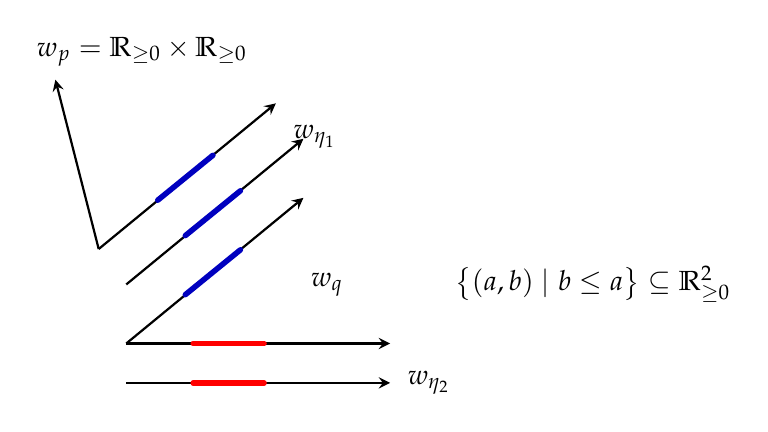
\begin{tikzpicture}[
        x=1cm,
        y=1cm,
        cone ray/.style={thick,->,>=stealth},
        common face/.style={red,line width=2pt,line cap=round},
        diagonal face/.style={blue!75!black,line width=2pt,line cap=round}
    ]
        % The cone at the marked point.
        \coordinate (p) at (0,4.45);
        \draw[cone ray] (p) -- ++(-0.55,2.15);
        \draw[cone ray] (p) -- ++(2.25,1.85);
        \draw[diagonal face]
            ($(p)+(0.75,0.62)$) -- ($(p)+(1.45,1.19)$);
        \node[above] at ($(p)+(0.55,2.2)$)
            {$w_p=\R_{\geq 0}\times\R_{\geq 0}$};

        % The cone at the first generic point.
        \coordinate (etaone) at (0.35,4);
        \draw[cone ray] (etaone) -- ++(2.25,1.85);
        \draw[diagonal face]
            ($(etaone)+(0.75,0.62)$) -- ($(etaone)+(1.45,1.19)$);
        \node[above right] at ($(etaone)+(2.0,1.6)$) {$w_{\eta_1}$};

        % The cone at the node.
        \coordinate (q) at (0.35,3.25);
        \draw[cone ray] (q) -- ++(2.25,1.85);
        \draw[cone ray] (q) -- ++(3.35,0);
        \draw[diagonal face]
            ($(q)+(0.75,0.62)$) -- ($(q)+(1.45,1.19)$);
        \draw[common face] ($(q)+(0.85,0)$) -- ($(q)+(1.75,0)$);
        \node at ($(q)+(2.55,0.75)$) {$w_q$};
        \node[anchor=west] at ($(q)+(4.05,0.75)$)
            {$\bigl\{(a,b)\mid b\leq a\bigr\}\subseteq\R_{\geq 0}^{2}$};

        % The colored intervals indicate the common faces used in the gluing.
        \coordinate (etatwo) at (0.35,2.75);
        \draw[cone ray] (etatwo) -- ++(3.35,0);
        \draw[common face] ($(etatwo)+(0.85,0)$) -- ($(etatwo)+(1.75,0)$);
        \node[right] at ($(etatwo)+(3.45,0)$) {$w_{\eta_2}$};
    \end{tikzpicture}
\end{figure}


\subsection{热带曲线}%
\label{sub:Tropical curves}

\begin{defn}
    锥\(w, N_w\)上的一个\textit{热带曲线}族\((G, \vec{g}, \vec{\ell})\)由以下数据组成：
    \begin{enumerate}
        \item 连通图\(G = V(G) \cup E(G) \cup L(G)\)；
        \item 腿的排序\(\vec{m} \colon L(G) \xrightarrow{\sim} \ab\{1, \ldots, n\}\)；
        \item 亏格函数\(\vec{g} \colon V(G) \to \N\)；
        \item 边长函数\(\ell \colon E(G) \to \Hom(w \cap N_w, \N) \setminus \ab\{0\}\)。
    \end{enumerate}
\end{defn}

现在我们构造\(\Sigma(G, \ell)\)。对\(v \in V(G)\)，令\(w_v = w\)。对\(e \in E(G)\)，令
\[ w_e = \ab\{ (s, \lambda) \mid \lambda \leq \vec{\ell}(e)(s) \} \subseteq w \times \R_{\geq 0}. \]
对腿\(\ell \in L(G)\)，令\(w_{\ell} = w \times \R_{\geq 0}\)。我们现在需要定义面映射。若\(\ell\)与\(v\)相邻接，则面映射是
\[ w_v \hookrightarrow w_{\ell} \colon s \mapsto (s, 0). \]
若\(e\)与两个顶点\(v_1, v_2\)相邻接，则面映射是
\begin{align*}
    w_{v_1} \hookrightarrow w_e &\colon s \mapsto (s, \vec{\ell}(e)(s)) \\
    w_{v_2} \hookrightarrow w_e & \colon s \mapsto (s, 0).
\end{align*}
\begin{rmk}
    \(v_1\)与\(v_2\)的选取在同构意义下不改变锥复形，但当我们想为对数映射定义接触阶时这个选取是有影响的。然而，一般来说没有典范的方式来作这个选取。
\end{rmk}

\subsection{穿孔曲线}%
\label{sub:Punctured curves}

穿孔对数曲线与穿孔对数映射的理论建立于~\cite{ACGS2025}。

我们考虑结点曲线
\[ \Spec k[x,y]/xy \to \Spec k \]
其对数结构由带图卡\((a,b) \mapsto x^a y^b\)的\(\N^2\)给出，而\(\N \to k\)是标准对数点。现在考虑\(\ul{C}_1 = Z(x) = \Spec k[y]\)，并用\(p \colon \Spec k \to \Spec k[y]\)标记该结点。注意
\[ C^{\on{can}} = (\ul{C}, M_C) \to S^{\on{can}} = \Spec(\N \to k). \]
记\(M_{C_1}^{\circ} = M_C|_{C_1}\)。那么我们看到在对数结构上有图表
\begin{equation*}
\begin{tikzcd}
    k[y] & & \N^2 \ar{ll}[swap]{(a,b) \mapsto 0^a y^b} \\
    k \ar{u} & & \N \ar{ll} \ar{u}{\Delta}.
\end{tikzcd}
\end{equation*}
特别地，我们可以计算茎\(\bar{M}_{C_1}^{\circ}|_p = \N^2\)，因此我们有
\[ \bar{\pi}_{C_1^{\circ}}^{\flat} |_p \colon \N \xrightarrow{\Delta} \N^2. \]
然而，我们本应有映射
\[ \bar{\pi}^{\flat}_{C_1}|_p \colon \N \xrightarrow{i_1} \N \oplus \N, \]
因此\(C_1\)\textbf{不是}对数曲线。然后我们可以考虑图表
\begin{equation*}
\begin{tikzcd}
    \N \oplus \Z \\
    \N^2 \ar[hookrightarrow]{u} \ar{rr}{(0,1)\mapsto (0,1)}[swap]{(1,0)\mapsto (1,1)} & & \N^2 \ar{ull}[swap]{\Vectorstack{{(1,0)\mapsto(1,-1)} {(0,1)\mapsto(0,1)}}} \\
    & \N \ar{ul}{i_1} \ar{ur}{\Delta}.
\end{tikzcd}
\end{equation*}
因此，我们将考虑扩张对数结构。

回忆对于对数曲线，我们有\(M_{\mc{C}} = M_{\mc{C}}' \oplus_{\mc{O}_{\mc{C}}^{\times}} P_{\mc{C}}\)，其中\(P_{\mc{C}}\)是由标记给出的除子对数结构。

\begin{defn}
    fs 对数概形\(S\)上的一条\textit{穿孔曲线}由\((\mc{C}^{\circ} \xrightarrow{p} \mc{C} \xrightarrow{\pi} S, \{p_i\}_{i=1}^n)\)组成，其中\((\mc{C} \xrightarrow{\pi} S, \vec{p})\)是对数曲线，而映射\(p \colon \mc{C}^{\circ} \to \mc{C}\)是精细对数概形的映射，满足以下条件：
    \begin{enumerate}
        \item 底映射\(\ul{p}\)是同构；
        \item 在对数结构上，映射\(p^{\flat} \colon M_{\mc{C}} \hookrightarrow M_{\mc{C}^{\circ}}\)在\(p_i\)之外是同构，并诱导
            \[ M_{\mc{C}} \xrightarrow{p^{\flat}} M_{\mc{C}^{\circ}} \hookrightarrow M_{\mc{C}} \oplus P^{\mr{gp}}. \]
        \item 对任何标记\(p_i\)与任何\(s \in M_{\mc{C}^{\circ}, p_i} \setminus M_{\mc{C}, p_i}\)，我们有\(\alpha_{\mc{C}^{\circ}}(s) = 0\)。
    \end{enumerate}
\end{defn}

粗略地说，穿孔曲线是对数曲线加上一个交换图表
\begin{equation*}
\begin{tikzcd}
    M_{\mc{C}^{\circ}} \ar{dr} \ar[hookrightarrow]{r} & M_{\mc{C}}' \oplus_{\mc{O}_{\mc{C}}^{\times}} P^{\on{gp}} \\
    & \mc{O}_{\mc{C}} \\
    M_{\mc{C}} \ar[hookrightarrow]{uu} \ar{ur}.
\end{tikzcd}
\end{equation*}
的数据。


\begin{exm}
    设\((\ul{\mc{C}} \to \ul{S} = \Spec k, p)\)是光滑的\(1\)-点曲线。
    \begin{enumerate}
        \item 给\((\mc{C}/S, p)\)赋予典范对数结构（因此\(S\)没有对数结构）。令\(M_{\mc{C}} = P\)。那么任何穿孔\(p^{\flat} \colon M_{\mc{C}} \hookrightarrow M_{\mc{C}^{\circ}} \subset P^{\on{gp}}\)必定是平凡的。原因是\(M_{\mc{C}^{\circ}}\)不可能有截面\(s\)使得\(\alpha_{\mc{C}^{\circ}}(s) = 0\)。若\(s \in P = M_{\mc{C}}\)，则\(\alpha_{\mc{C}^{\circ}}(s) = \alpha_{\mc{C}}(s)\)。否则，若\(s \notin P\)，则由于\(\alpha_{\mc{C}^{\circ}}(-s)\)非零，\(\alpha_{\mc{C}^{\circ}}(s)\)也非零。
        \item 设\(M_{\mc{C}^{\circ}} \subseteq (\N \oplus \mc{O}_{\mc{C}}^{\times}) \oplus P^{\on{gp}}\)是一个穿孔。选取\(\mc{O}(-p)\)的一个局部生成元\(x\)。那么任何\(s \in M_{\mc{C}^{\circ}, p}\)都形如\(s = ((n, \varphi), x^m)\)，其中\(n \in \N\)且\(\varphi \in \mc{O}_{\mc{C}, p}^{\times}\)。若\(m < 0\)，则我们要求\(\alpha_{\mc{C}^{\circ}}(s) = 0\)。这蕴含\(\alpha_{\mc{C}}((n, \varphi), 0) = 0\)，因此
            \[ \bar{M}_{\mc{C}^{\circ}, p} \subseteq \ab\{(n, m) \in \N \oplus \Z \mid m \geq 0 \text{若} n = 0 \}. \]
            事实上，右端任何包含\(\N \oplus \N\)的精细子幺半群都可以由某个穿孔实现。
        \item 令\(S = \Spec(\N \to k)\)。考虑满足\(\bar{M}_{\mc{C}^{\circ}, p} = \N^2 + \N (2,-2)\)的\(M_{\mc{C}^{\circ}}\)。由于\((1,-1) \notin \bar{M}_{\mc{C}^{\circ}, p}\)，我们看到\(M_{\mc{C}^{\circ}}\)不是饱和的。
    \end{enumerate}
\end{exm}

\begin{lem}[{\cite{ACGS2025}}]
    设\(Q\)是尖的 fs 幺半群。令\(w \coloneqq \Hom(Q, \R_{\geq 0}) = Q_{\R}^{\vee}\)。设\(Q^{\circ} \subseteq Q \oplus \Z\)有限生成，满足\(Q \oplus \N \subsetneq Q^{\circ}\)且\(Q^{\circ} \cap \ab\{0\} \times \Z_{<0} = \emptyset\)。那么存在一个非零的、凹的、分片线性的函数
    \[ \ell \colon w \to \R_{\geq 0} \]
    具有有理斜率，使得
    \[ (Q^{\circ})_{\R}^{\vee} = \ab\{ (s, \lambda) \in w \times \R_{\geq 0} \mid 0 \leq \lambda \leq \ell(s) \}. \]
\end{lem}

\begin{exm}
    令\(Q = \N^2\)，并令
    \begin{align*}
        Q^{\circ} &= \ab<((1,0), -1), ((0,1), -1), ((0,0),1)> \subset \N^2 \oplus \Z \\
        &= \ab\{((a,b), m) \mid a+b+m \geq 0, a,b \geq 0 \}.
    \end{align*}
    那么
    \[ (Q^{\circ})_{\R}^{\vee} = \ab\{ (e_x, e_y, e_t) \mid 0 \leq e_t \leq \min(e_x, e_y) \}. \]
\end{exm}





\section{面向高亏格的 GW 理论简介（Patrick Lei）}%
\label{sec:Intro to GW theory with a view to higher genus (Patrick Lei)}


\subsection{GW 理论简介}%
\label{sub:Introduction to GW theory}

关于虚基本类的构造，参见~\cite{BehrendFantechi1997}；关于公理与量子上同调，参见~\cite{KM1994}。

这几次讲座的目标是以一种便于进行高亏格计算的方式来讨论 Gromov-Witten 理论。Gromov-Witten 理论关注的是模空间\(\Mbar_{g,n}(X, \beta)\)上的积分，其中\(X\)是光滑射影代数簇，\(\beta \in H_2(X, \Z)\)是有效曲线类。我们有图表
\begin{equation*}
\begin{tikzcd}
    \mc{C} \ar{r}{f} \ar[bend right=20]{d}[swap]{\pi} & X \\
    \Mbar_{g,n}(X, \beta) \ar[bend right=20]{u}[swap]{\sigma_i} \ar{ur}[swap]{\on{ev}_i}
\end{tikzcd}
\end{equation*}
其中\(\mc{C}\)是泛曲线，\(\sigma_i\)是\(\pi\)的给出标记点的截面，\(f\)是泛稳定映射，而\(\ev_i = f \circ \sigma_i\)是赋值态射。虽然\(\Mbar_{g,n}(X, \beta)\)一般是奇异的、非等维的且可约的，但存在一个特殊的类
\[ [\Mbar_{g,n}(X, \beta)]^{\vir} \in A_{\ab(c_1(X), \beta) + (\dim X - 3)(1-g) + n}(\Mbar_{g,n}(X, \beta), \Q), \]
称为\textit{虚基本类}。

\begin{exer}
    用形变理论的标准论证验证\(\Mbar_{g,n}(X, \beta)\)的“期望维数”就是上面给出的数。
\end{exer}

在\(X\)光滑射影的假设下，\(\Mbar_{g,n}(X, \beta)\)是紧合的，因此我们可以定义\textit{GW 不变量}
\[ \ab<\tau_{a_1}(\alpha_1), \cdots, \tau_{a_n}(\alpha_n)>_{g,n,\beta} \coloneqq \int_{[\Mbar_{g,n}(X, \beta)]^{\vir}} \prod_{i=1}^n \ev_i^* \alpha_i \cdot \psi_i^{a_i} \]
其中\(\alpha_i \in H^*(X)\)。这里\(\psi_i\)定义为\(\psi_i = c_1(\sigma_i^*(\omega_{\pi}))\)。

不幸的是，计算单个 Gromov-Witten 不变量非常困难，所以我们将考虑一个更困难的问题，即研究 GW 不变量的生成级数，例如当\(X\)是 Calabi-Yau 三维流形时的
\[ F_g = \sum_{\beta \geq 0} q^{\beta} \ab<>_{g,0,\beta} \]
这里\(q\)是记录曲线类的形式变量，我们将环\(\Q\ps{q^{\beta} \mid \beta \in H_2(X, \Z)_{\mr{eff}}}\)记为\(\Lambda\)。我们还会考虑一些其他的结构。首先，我们可以考虑\textit{量子上同调环}，其乘积\(a \star_{\mbf{t}} b\)由公式
\[
    (a \star_{\mbf{t}} b, c) = \sum_{\substack{\beta \geq 0 \\ n \geq 0}} \ab<a,b,c, \mbf{t}, \ldots, \mbf{t}>_{0,3+n,\beta} \frac{q^{\beta}}{n!}.
\]
给出。这里\(a,b,c, \mbf{t} \in H^*(X)\)。我们还将考虑\textit{量子联络}。设\(\ab\{ e_i \}\)是\(H^*(X)\)的一组基。那么量子联络是\(H^*(X) \times \P^1_z\)上纤维为\(H^*(X)\)的平凡丛上的联络，由公式
\[ \nabla_{t^i} = \partial_{t^i} + \frac{1}{z} e_i \star_{\mbf{t}}. \]
给出。有时考虑\(z\)-方向上的联络也是有用的，它由
\[ \nabla_{z \odv{}{z}} \coloneqq z \odv{}{z} - \frac{1}{z} E_X \star_{\mbf{t}} + \mu_X, \]
给出，其中\(\mu_X(\alpha) = \frac{\deg(\alpha) - \dim X}{2} \alpha\)是分次算子，而
\[ E_X = c_1(X) + \sum_i \ab(1 - \frac{\deg(e_i)}{2})t^i e_i \]
是\textit{Euler 向量场}。由于我们主要关心 Calabi-Yau 簇，我们不会考虑这个。

\subsection{亏格零的计数镜像对称}%
\label{sub:Enumerative mirror symmetry in genus zero}

数学家发展并研究 Gromov-Witten 理论的动力来自 20 世纪 90 年代初，当时 Candelas、de la Ossa、Green 与 Parkes~\cite{CandelasEtAl1991}通过把问题转化为在另一个称为\textit{镜像五次}的 Calabi-Yau 三维流形上计算周期积分（等价地，研究其 Hodge 结构的变分），预言了一般五次三维流形上低次有理曲线的数目。在亏格零，所有不变量都可以从\textit{J-函数}\(J_{\mbf{t}}(q,z) \in H^*(X, \Lambda)[z]\)中恢复出来，它由
\[ \ab( J_{\mbf{t}}(q, z), \alpha ) \coloneqq (z + \mbf{t}, \alpha) + \sum_{n, \beta} \frac{q^{\beta}}{n!} \ab< \frac{\alpha}{z-\psi}, \mbf{t}, \ldots, \mbf{t}>_{0,1+n, \beta} \]
定义，其中\(\mbf{t} \in H^*(X, \Lambda)[z]\)与\(\alpha \in H^*(X)\)任意，而\((-,-)\)是 Poincar\'e 配对。因此，计算所有带后代（即\(\psi\)-类）的亏格零 Gromov-Witten 不变量的问题归结为计算 J-函数的问题。

\begin{rmk}
    我们把\(\frac{1}{z-\psi}\)展开为\(\sum_{k=0}^{\infty} \psi^k z^{-k-1}\)。
\end{rmk}

我们应当指出，J-函数可以通过量子微分方程的一个基本解得到，该基本解由
\[ ( S_{\mbf{t}}(z) \phi , \alpha) = (\phi, \alpha) + \sum_{n, \beta} \frac{q^{\beta}}{n!} \ab<\frac{\alpha}{z-\psi}, \phi, \mbf{t}, \ldots, \mbf{t}>_{0, 2+n, \beta}. \]
给出。它满足性质\(S_{\mbf{t}}^*(-z) S_{\mbf{t}}(z) = \on{Id}\)，通常称为\textit{辛性质}。由此，我们可以通过\(z S_{\mbf{t}}^*(z)\cdot 1 = J_{\mbf{t}}(q, z)\)恢复 J-函数。

在物理中，镜像对称是两个不同理论（称为 A-模型与 B-模型）之间的对偶，所以现在我们需要引入 B-模型的对象。为了节省时间（以及记号），我们假设\(X\)是环面簇且\(-K_X\)是 nef 的。设\(D_1, \ldots, D_r\)是\(X\)中全部环面不变除子。定义\(I\)-函数
\[
    I_{\mbf{t}}(q, z) \coloneqq z e^{\mbf{t}/z} \sum_{\beta \geq 0} q^{\beta} \frac{\prod_{i=1}^r \prod_{m = -\infty}^{0} (D_i + mz)}{\prod_{i=1}^r \prod_{m=-\infty}^{\beta \cdot D_i} (D_i + mz)}.
\]
注意这里我们把出现的任何\((D_i + mz)^{-1}\)展开为\(\frac{1}{mz} \ab(1 - \frac{D_i}{mz} + \cdots)\)，也就是关于\(\frac{D_i}{mz}\)的几何级数。此外，I-函数被一个称为 \textit{Picard-Fuchs 方程}的微分方程零化，它是某种超几何型方程。

\begin{exm}
    若\(\mbf{t} = 0\)且\(X = \P^1\)，我们得到
    \begin{align*}
        I(q,z) &= z\sum_{d \geq 0} q^d \frac{1}{\prod_{m=1}^d (H + mz)^2} \\
        &= z\sum_{d \geq 0} \ab(\frac{q}{z^2})^d \frac{1}{(d!^2)} + O(H),
    \end{align*}
    所以事实上我们看到首项是第一类 Bessel 函数。
\end{exm}

若\(X\)是环面簇\(Y\)中由线丛\(L_1, \ldots, L_k\)切出的完全交，且对到\(Y\)的任意亏格零稳定映射都满足\(H^1(f^* L_i) = 0\)（这称为\textit{凸}），那么量子 Lefschetz 定理~\cite{CoatesGivental2007}允许我们把\([\Mbar_{g,n}(X, \beta)]^{\vir}\)替换为\(e\ab(\bigoplus \pi_* f^* L_i) \cap [\Mbar_{g,n}(Y, \beta)]^{\vir}\)，并在\(Y\)上进行所有计算。此时，I-函数定义为
\[
    I_{\mbf{t}}(q,z) \coloneqq z e^{\mbf{t}/z} \sum_{\beta \geq 0} q^{\beta} \frac{\prod_{i=1}^k \prod_{m=-\infty}^{L_i \cdot \beta} (L_i + mz)}{\prod_{i=1}^k \prod_{m=-\infty}^{0} (L_i + mz)} \frac{\prod_{i=1}^r \prod_{m = -\infty}^{0} (D_i + mz)}{\prod_{i=1}^r \prod_{m=-\infty}^{\beta \cdot D_i} (D_i + mz)},
\]
这里我们滥用记号，把\(L_i\)与其第一陈类等同。

\begin{exm}
    对于由\(\mc{O}_{\P^4}(5)\)的一个截面切出的五次三维流形，\(\mbf{t} = 0\)处的 I-函数由
    \[ I(q,z) = z \sum_{d \geq 0} q^d \frac{\prod_{m=1}^{5d}(5H+mz)}{\prod_{m=1}^d (H+mz)^5}. \]
    给出。
\end{exm}

亏格零镜像定理的内容是这两个对象之间的一个对应。更确切地说，在\(-K_X\)为 nef 的情形，它们通过一个变量替换相联系。

\begin{thm}[{\cite{Givental1998,LLY1997}}]
    把\(\mbf{t} = 0\)时的 I-函数写成\(I_0(q) \cdot z + I_1(q) + O(z^{-1})\)。那么我们有
    \[
        J_{\tau(\mbf{t})}(q,z) = \frac{I_{\mbf{t}}(q,z)}{I_0(q)},
    \]
    其中\(\tau(\mbf{t}) = \frac{\mbf{t} + I_1(q)}{I_0(q)}\)。
\end{thm}

\begin{exm}
    当\(X = \P^1\)时，注意\(I_0(q) = 1\)且\(I_1(q) = 0\)，所以事实上我们有等式
    \[ J_{\mbf{t}}(q,z) = I_{\mbf{t}}(q,z). \]
\end{exm}

\begin{exm}
    当\(X\)是五次三维流形时，为方便起见我们把 I-函数的各分量改写为\(I_0(q) \cdot z + I_1(q)H + O(z^{-1})\)。我们有
    \[ I_0(q) = \sum_{d \geq 0} \frac{(5d)!}{(d!)^5} q^d, \qquad I_1(q) = \sum_{d \geq 0} \frac{(5d)!}{(d!)^5} \ab(5\sum_{m=d+1}^{5d} \frac{1}{m}) q^d, \]
    所以此时存在非平凡的镜映射。特殊化到\(\mbf{t} = 0\)，我们看到\(\tau = \frac{I_1(q)H}{I_0(q)}\)，从而得到
    \[ J_{\tau}(q,z) = \frac{I(q,z)}{I_0(q)}. \]
    由除子方程，左边也等于\(J(qe^{I_1/I_0}, z)\)，我们也把这称为镜映射。
    因此，我们可以用镜像定理来计算$\star_{\tau}$。沿\(H^2\)方向的量子联络成为常微分方程
    \[ (H+zD) S_{\tau}(z)^* = S_{\tau}(z)^* \cdot I_{11} H \star_{\tau}, \]
    其中$D \coloneqq q \odv{}{q}$（这里坐标是$\log q$），$I_{11} \coloneqq 1 + D \ab(\frac{I_1(q)}{I_0(q)})$。利用镜像定理和 Zagier-Zinger 的结果~\cite{ZagierZinger2008}直接计算可得
    \begin{align*}
        I_{11} H + \cdots &= S_{\tau}(z)^* (I_{11} H \star_{\tau} \1) \\
        \ab( 1 + D\ab(\frac{\frac{I_1}{I_0} + D \ab(\frac{I_2}{I_0})}{I_{11}}) ) H^2 + \cdots &= S_{\tau}(z)^* (I_{11} H \star_{\tau} H) \\
        I_{11} H^3 &= S_{\tau}(z)^* (I_{11}H \star_{\tau} H^2).
    \end{align*}
    由于$S_{\tau}$以恒等开头，这就计算出了$H \star_{\tau}$。
\end{exm}

\subsubsection{振荡积分}%
\label{ssub:Oscillating integrals}

现在我们重新诠释亏格零镜像定理，并且在讨论高亏格不变量时我们还会回到这一诠释。特别地，我们将把 I-函数解释为\(X\)的某个镜像族上的积分，这里\(X\)是环面簇。设
\[ 0 \to \Lambda \to \Z^r \to N \to 0 \]
是\(X\)的扇序列。应用\(\Hom(-, \C^{\times})\)，我们得到正合列
\[ 1 \to (\C^{\times})^{\dim X} \to (\C^{\times})^r \to \Hom(\Lambda, \C^{\times}) \to 1. \]
假设映射\(\Lambda \to \Z^r\)由矩阵\((m_{ij})_{i=1,\ldots,r}^{j = 1, \ldots, \rho(X)}\)给出。那么我们考虑簇
\[ E_q = \ab(\prod_{i=1}^r x_j^{m_{ij}} = q_i \middle\vert i=1, \ldots, \rho(X)) \]
它是\(X\)的镜像，并考虑超势\(f = x_1 + \cdots + x_r\)。若我们想考虑等变理论，其中等变参数\(\lambda_1, \ldots, \lambda_r\)作用在\(X\)的每个齐次坐标上，我们将考虑\(f_{\lambda} = \sum_{i=1}^r (x_i - \lambda_i \log x_i)\)。

\begin{exm}
    当\(X = \P^n\)时，\(X\)的镜像是簇\(E_q = (x_1 \cdots x_{n+1} = q)\)上的超势\(\sum_{i=1}^{n+1} (x_i - \lambda_i \log x_i)\)。
\end{exm}

现在我们在（等变）超势的每个临界点\((x_{\alpha})\)附近选取一个合适的 Lefschetz 顶针\(\Gamma_{\alpha}\)，并考虑积分
\[ I_{\alpha} = \int_{\Gamma_{\alpha}} e^{f_{\lambda}/z} \prod_{i=1}^r \frac{\d{x_i}}{x_i}. \]
在 I-函数一侧，这对应于把表达式中的每个\(D_i\)替换为\(D_i - \lambda_i\)（打开等变参数）；在 J-函数一侧，这对应于考虑\(X\)的完全等变 GW 理论。在亏格零，\(\lambda_i \to 0\)的极限存在，所以我们可以放心地从下面的结果恢复原来的镜像定理：

\begin{thm}[{\cite{Givental1996}}]
    这个积分被与 I-函数相同的 Picard-Fuchs 方程零化，并且在相差若干前置因子的意义下，它沿负实轴\(z \to 0^-\)时的渐近展开与 I-函数在\(X\)上对应于临界点\(( x_{\alpha} )\)的 T-不动点处的限制相吻合。
\end{thm}


\subsubsection{Lagrange 锥}%
\label{ssub:The Lagrangian cone}

\(X\)的量子上同调是 \textit{Frobenius 流形}的一个例子，我们稍后会看到任何上同调场论都能产生 Frobenius 流形。记\(V = H^*(X)\)，设\((e_{\mu})\)是\(V\)的一组基，于是我们可以写$\bv = \sum_{\mu,n} t^{\mu}_n e_{\mu} z^n \in V\ps{z}$。
Frobenius 流形的结构来自函数
\[
    \mc{F}_0(\bv) = \sum_{n, \beta, \mu} \frac{q^{\beta}}{n!} \ab<\bv(\psi), \ldots, \bv(\psi)>_{0,n,\beta},
\]
它也称为\(X\)的\textit{亏格零后代势}。它满足弦方程、膨胀子方程以及拓扑递归关系：
\begin{align*}
    \pdv{}{t_0^1} \mc{F}_0 &= \frac{1}{2} (\bv_0, \bv_0) + \sum_{n=0}^{\infty} \sum_{\mu} t_{n+1}^{\mu} \pdv{}{t_n^{\mu}} \mc{F}_0; \\
    \pdv{}{t_1^1} \mc{F}_0 &= \sum_{n=0}^{\infty} \sum_{\mu} t_n^{\mu} \pdv{}{t_n^{\mu}}\mc{F}_0 - 2 \mc{F}_0; \\
    \pdv{}{t_{k+1}^{\alpha},t_m^{\beta},t_n^{\gamma}} \mc{F}_0 &= \sum_{\mu,\nu} \pdv{}{t_k^{\alpha},t_0^{\mu}} \mc{F}_0 \cdot \eta^{\mu\nu} \cdot \pdv{}{t_0^{\nu},t_{m}^{\beta},t_n^{\gamma}} \mc{F}_0.
\end{align*}
为了叙述下面的结果，我们考虑无穷维向量空间$V\ls{z^{-1}}$（或其某个完备化），带有辛形式
\[ \omega(\mbf{f}(z), \mbf{g}(z)) \coloneqq \on{Res}_{z=0}(\mbf{f}(-z), \mbf{g}(z)). \]
我们还考虑新变量\footnote{这称为\textit{膨胀子平移}。}$\bq = \bv - z$，于是$\mc{F}_0$现在是$\bq = -z$附近的函数。

\begin{thm}[Givental {\cite{Givental2004}}]
    $\mc{F}_0$满足上述偏微分方程当且仅当$\d{\mc{F}_0}$的图像$\mc{L}$是顶点在$\bq = 0$的 Lagrange 锥，且其切空间$L$恰好沿$zL \subset L$与$\mc{L}$相切。
\end{thm}

我们可以通过如下步骤恢复 Lagrange 锥$\mc{L}$。我们找到量子联络的一个基本解
\[ S = \mr{Id} + S_1 z^{-1} + S_2 z^{-2} + \cdots \]
它满足方程
\[ z \pdv{}{t^{\mu}}S = e_{\mu} \star S. \]
然后，令$J \coloneqq z S^*(z) \1$，我们便可以通过如下步骤恢复 Lagrange 锥：
\begin{itemize}
    \item 导数$\pdv{}{t^{\mu}} J$构成$L \cap V\ps{z^{-1}}$的一组基；
    \item 这蕴含$z \pdv{}{t^{\mu},t^{\nu}} J \in L \cap V \ps{z^{-1}}$。把它们用一阶导数表示出来，并利用$J$是量子联络的解这一事实，我们就恢复了 Frobenius 结构，从而恢复了 Lagrange 锥。
\end{itemize}

利用这一点，我们可以把亏格零镜像定理解释为：
\begin{thm}[{\cite{Givental1998}}]
    I-函数\(I_{\mbf{t}}(q,z)\)落在\(X\)的 Lagrange 锥上。
\end{thm}




\subsection{曲线模空间与 CohFT}%
\label{sub:Moduli of curves and CohFTs}

上同调场论的概念由 Kontsevich-Manin~\cite{KM1994}引入。

我们用$\Mbar_{g,n}$表示亏格$g$带$n$个标记点的稳定曲线的模空间。它非空当且仅当$2g-2+n > 0$，此时它是维数为$3g-3+n$的 Deligne-Mumford 叠。全体$\Mbar_{g,n}$上有一个组合结构，由一族态射给出。
\begin{itemize}
    \item 有粘合态射
        \[q \colon \Mbar_{g,n+1} \times \Mbar_{h, m+1} \to \Mbar_{g+h,n+m}, \]
        它取两条曲线并沿最后一个标记点把它们粘合成一个结点；
    \item 有自粘合态射\[s \colon \Mbar_{g-1,n+2} \to \Mbar_{g,n},\]
        它把最后两个标记点粘合起来。
\end{itemize}
当然还有另一个有趣的映射，即忘却映射
\[ \pr \colon \Mbar_{g,n+1} \to \Mbar_{g,n} \]
它由删去最后一个标记点再稳定化给出。现在我们可以定义我们感兴趣的计数理论，其中包括 Gromov-Witten 理论。

\begin{defn}
    给定带非退化对称双线性形式$\eta$和单位元$\1 \in V$的向量空间$V$，$V$上的\textit{上同调场论（CohFT）}$\Omega$是一族$S_n$-等变线性映射
    \[ \Omega_{g,n} \colon V^{\otimes n} \to H^*(\Mbar_{g,n}) \]
    满足基本恒等式
    \[ \Omega_{0,3}(\1, u,v) = \eta(u,v) \]
    以及下列组合恒等式（我们取$V$的一组基$e_{\mu}$使得$e_1 = \1$，并取$e^{\mu}$为对偶基）：
    \begin{align*}
        q^* \Omega_{g+h,n+m}(\bv_1, \bv_2) &= \sum_{\mu} \Omega_{g,n+1}(\bv_1, e_{\mu}) \cdot \Omega_{h,m+1}(  \bv_2, e^{\mu} ); \\
        s^* \Omega_{g,n}(\bv) &= \sum_{\mu} \Omega_{g,n+2}(\bv, e_{\mu}, e^{\mu}).
    \end{align*}
    若此外恒等式
    \[ \pr^*\Omega_{g,n}(\bv) = \Omega_{g,n+1}(\bv,\1) \]
    也成立，则我们说该 CohFT 具有\textit{平坦单位}（或满足\textit{弦方程}）。
\end{defn}
所有这些都可以推广到超向量空间，但为简单起见我们不处理这种情形。

\begin{exm}
    CohFT 最重要的例子是光滑射影簇$X$的 Gromov-Witten 理论。这里回忆稳定映射的源是一条\textbf{预稳定}曲线，所以存在稳定化态射
    \[ \st \colon \Mbar_{g,n}(X,\beta) \to \Mbar_{g,n} \]
    它忘掉映射并把曲线稳定化。然后，在 Novikov 环上工作，我们令$V = H^*(X)$，$\eta$为 Poincar\'e 配对，$\1$为$X$的基本类。线性映射$\Omega^X_{g,n}$由公式
    \[ \Omega_{g,n}^X(\btau) \coloneqq \sum_{\beta} q^{\beta} \st_* \ab(\prod_{i=1}^n \ev_i^*(\tau_i) \cap [\Mbar_{g,n}(X,\beta)]^{\vir}), \]
    给出，其中$\ev_i \colon \Mbar_{g,n}(X,\beta) \to X$是第$i$个赋值映射。
\end{exm}

\begin{exm}
    设$\pi \colon \mc{C}_{g,n} \to \Mbar_{g,n}$是泛曲线。那么 \textit{Hodge 丛}是向量丛
    \[ \E_{g,n} \coloneqq \pi_* \omega_{\pi}. \]
    然后我们考虑带通常配对的向量空间$V = \C$，并通过公式
    \[ \Omega^{\E}_{g,n} \coloneqq c(\E_{g,n}). \]
    定义 CohFT $\Omega^{\E}$。粘合公理由等式$q^* \E_{g+h} = \E_g \oplus \E_h$和正合列
    \[ 0 \to \E_{g-1} \to \E_g \to \mc{O} \to 0. \]
    保证。这里，由于亏格零分支对$\omega$的整体截面没有贡献，且$\E$不依赖于标记点，这个 CohFT 具有平坦单位。
\end{exm}

\begin{rmk}
    我们稍后会看到，通过量子 Riemann-Roch 定理，它与一个点的 GW CohFT 相关联。
\end{rmk}

给定 CohFT $\Omega$，我们可以把类$\Omega_{g,n}(\bv)$与$\Mbar_{g,n}$上的各种上同调类配对来产生不变量。最重要的是类
\[ \bar{\psi}_i \coloneqq c_1( s_i^* \omega_{\pi} ), \]
其中$s_i \colon \Mbar_{g,n} \to \mc{C}_{g,n}$是第$i$个标记点。

\begin{rmk}
    在 Gromov-Witten 理论中，这些称为\textit{祖先}。还有后代，它们由同样的公式给出，只是用预稳定曲线的模空间$\mf{M}_{g,n}$代替$\Mbar_{g,n}$，这里我们把上面定义的态射$\st$分解为
    \[ \Mbar_{g,n}(X,\beta) \xrightarrow{\text{忘却映射}} \mf{M}_{g,n} \xrightarrow{\text{稳定化}} \Mbar_{g,n}. \]
    后代类记为$\psi_i$。
\end{rmk}

\begin{exm}
    我们来计算一个会出现在 Calabi-Yau 三维流形 GW 理论中的不变量。对任意 CohFT $\Omega$，考虑不变量
    \[ \ab<\1\bar{\psi}_1>_{1,1}^{\Omega}\coloneqq \int_{\Mbar_{1,1}} \Omega_{1,1}(\1)\bar{\psi}_1. \]
    利用第二个粘合方程，$\Omega_{1,1}(\1)$的零次部分等于
    \[ \sum_{\mu} \Omega_{0,3}(\1, e_{\mu}, e^{\mu}) = \sum_{\mu} \eta(e_{\mu}, e^{\mu}), \]
    这给出$V$的（分次）维数$\chi(V)$（例如，若\(V = H^*(X)\)，其中\(X\)是 Calabi-Yau 三维流形，那么这就是\(X\)的拓扑欧拉示性数）。因此，我们得到
    \[ \ab<\1\bar{\psi}_1>_{1,1}^{\Omega} = \frac{\dim V}{24}. \]
\end{exm}

\begin{exm}
    考虑一个点的 GW CohFT。它由带通常配对的$V = \C$以及公式
    \[ \Omega_{g,n} = 1. \]
    给出。然后我们定义不变量
    \[ \ab<\bar{\psi}_1^{a_1} \cdots \bar{\psi}_n^{a_n}>_{g,n} \coloneqq \int_{\Mbar_{g,n}} \Omega_{g,n} \cdot \bar{\psi}_1^{a_1} \cdots \bar{\psi}_n^{a_n}. \]
    \begin{thm}[Kontsevich {\cite{Kontsevich1992}}]
        函数
        \[ \mc{D} \coloneqq \exp \ab(\sum_{g,n} \frac{\hbar^{g-1}}{n!}\sum_{a_1 + \cdots + a_n = 3g-3+n} \ab<\bar{\psi}_1^{a_1} \cdots \bar{\psi}_n^{a_n}>_{g,n} t_{a_1}\cdots t_{a_n}) \]
        被算子
        \begin{align*}
            L_{-1} \coloneqq{}& -\pdv{}{t_0} + \frac{\hbar^{-1}}{2} t_0^2 + \sum_{i=0}^{\infty} t_{i+1} \pdv{}{t_i};\\
            L_0 \coloneqq{}& -\frac{3}{2} \pdv{}{t_1} + \sum_{i=0}^{\infty} \frac{2i+1}{2} t_i \pdv{}{t_i} + \frac{1}{16};\\
            L_n \coloneqq{}& -\frac{(2n+3)!!}{2^{n+1}} \pdv{}{t_{n+1}} + \sum_{i=0}^{\infty} \frac{(2i+2n+1)!!}{(2i-1)!! 2^{n+1}} t_i \pdv{}{t_{i+n}} \\
            &+ \frac{\hbar}{2} \sum_{i=0}^{n-1} \frac{(2i+1) (2i-1) \cdots (2i+1-2n)}{2^{n+1}} \pdv{}{t_i,t_{n-1-i}}.
        \end{align*}
        零化。
    \end{thm}
\end{exm}

\begin{rmk}
    这个结果（一个点的 Virasoro 约束）等价于$\mc{D}$是 KdV 族的 τ-函数，并已被多位作者推广。
\end{rmk}



\subsection{$R$-矩阵作用}%
\label{sub:R-matrix action}

21 世纪初，Givental 发现了公理化计数理论的一个引人注目的性质，即可以通过满足性质
\[ R^*(-z) R(z) = \mr{Id}_V. \]
的矩阵$R(z) = R_0 + R_1 z + R_2 z^2 + \cdots \in \Hom(V, V')\ps{z}$的作用来变换 CohFT。传统上，文献要求$V = V'$且$R_0 = \mr{Id}$，但 MSP 小组去掉了这一限制，并且也允许$\dim V < \dim V'$。

为了定义$R$在$V$上的 CohFT $\Omega$上的作用，我们需要回顾$\Mbar_{g,n}$的一些组合结构。对曲线$C\in \Mbar_{g,n}(\C)$，我们可以考虑$C$的对偶图，它有顶点、边和腿，定义如下：
\begin{itemize}
    \item 顶点对应$C$的不可约分支，并用一个非负整数标记，即亏格；
    \item 边对应$C$的结点（特别地，我们允许自环）；
    \item 腿对应标记点。
\end{itemize}
任何作为稳定曲线对偶图出现的图称为\textit{稳定图}。

\begin{figure}[htpb]
  \centering
  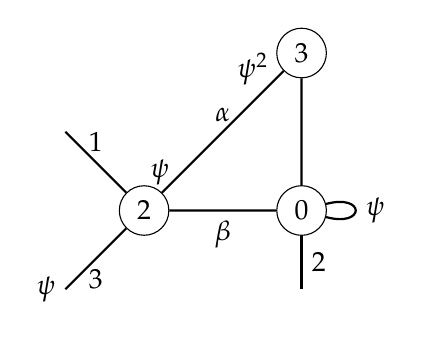
\begin{tikzpicture}[scale=1,transform shape,every loop/.style={}]
    \node[circle,draw] (A) at (0,0) {$2$};
    \node[circle,draw] (B) at (2,2) {$3$};
    \node[circle,draw] (C) at (2,0) {$0$};
    \draw[thick] (A) -- node[above]{$\alpha$} (B) -- (C) -- node[below]{$\beta$} (A);
    \draw[thick] (A) -- node[below]{$3$} (-1,-1);
    \draw[thick] (A) -- node[above]{$1$} (-1,1);
    \draw[thick] (C) -- node[right]{$2$} (2,-1);
    \draw[thick] (C) edge[loop right] node[right] {$\psi$} (C);
    \node[anchor=east] at (-1,-1) {$\psi$};
    \node[anchor=east] at (1.7,1.8) {$\psi^2$};
    \node[anchor=south] at (0.2,0.2) {$\psi$};
  \end{tikzpicture}
  \caption{$\ol{\mc{M}}_{7,3}$中稳定图及相应重言类的例子。该稳定图描述了映射
    $\ol{\mc{M}}_{2,4} \times \ol{\mc{M}}_{3,2} \times \ol{\mc{M}}_{0,5} \to \ol{\mc{M}}_{7,3}$的像。}
  \label{fig:stablegraph}
\end{figure}

CohFT 上的第一类作用是平移作用。设$T \in V\ps{z}$。对 CohFT $\Omega$，只要无穷和有意义，我们定义
\[ (T\Omega)_{g,n}(\bv) \coloneqq \sum_m \frac{1}{m!} p_* \Omega_{g,n+m}(\bv, T,\ldots,T) \]

\begin{exm}
    若$\Omega^X$是光滑射影簇$X$的 GW CohFT 且$\tau \in H^2(X)$是除子类，那么无穷和有意义，我们可以定义$X$的平移 GW CohFT $\Omega^{X,\tau}$。例如，若$X$是五次三维流形且$\tau = \frac{I_1}{I_0} H$，那么平移到$\tau$与镜映射$q \mapsto Q(q) = q e^{\frac{I_1}{I_0}}$是一回事。
\end{exm}

第二类作用是本节开头那样的矩阵$R$的作用。设$G_{g,n}$表示亏格$g$带$n$条腿的全体稳定图的集合。那么我们定义
\[ (R\Omega)_{g,n} \coloneqq \sum_{\Gamma \in G_{g,n}} \frac{1}{\ab|\Aut \Gamma|} \on{Cont}_{\Gamma}, \]
其中$\on{Cont}_{\Gamma}$由如下构造定义：
\begin{itemize}
    \item 在第$i$条腿上，我们放置映射
        \[ R(-\bar{\psi}_i)^* \in \Hom(V',V) \ps{\bar{\psi}_i}; \]
    \item 在每条边上，我们放置双向量
        \[ V(\bar{\psi}_1, \bar{\psi}_2) \coloneqq \sum_{\mu} \frac{e_{\mu} \otimes e^{\mu} - R(-\bar{\psi}_1)^* e_{\mu} \otimes R(-\bar{\psi}_2)^* e^{\mu}}{\bar{\psi}_1 + \bar{\psi}_2}; \]
    \item 在每个顶点上，我们放置线性映射
        \[ \Omega_{g_v, n_v} \colon V^{\otimes n_v} \to H^*(\Mbar_{g_v, n_v}); \]
    \item 最后，我们考虑沿粘合态射$\prod_v \Mbar_{g_v, n_v} \to \Mbar_{g,n}$的上同调推前。
\end{itemize}

\begin{defn}
    设$R$如上。那么我们定义平移
    \[ T_R \coloneqq z (\1 - R(-z)^* \1') \in z V\ps{z}. \]
    只要有意义，我们定义
    \[ R.\Omega \coloneqq RT\Omega. \]
\end{defn}

\begin{thm}[张怀良–郭帅–李骏 {\cite[定理~2.7]{CGL2026}}]
    假设我们在系数$\C\ps{q}$上工作。那么若
    \[ T_R \in z^2 V \ps{z} + zq V \ps{z}, \]
    则$R.\Omega$是良定义的 CohFT。此外，若$\dim V = \dim V'$，则$\1'$是$R.\Omega$的单位。
\end{thm}

我们想对$R_0 \neq \mr{Id}$时的平移作用再多说几句。为简单起见，我们假设$V = V'$且对某个常数$c$有$R_0 \1 = c \cdot \1$。那么我们令$\tilde{T}_R \coloneqq z( \1 - c R(z)^{-1} \1)$，并利用膨胀子方程计算
\begin{align*}
    T_R \Omega_{g,n}(\bv) &= \sum_{m=0}^{\infty} \frac{1}{m!} p_*\Omega_{g,n+m}(\bv, T_R, \ldots, T_R) \\
    &= \sum_{k,\ell \geq 0} \frac{1}{k!\ell!} p_* \Omega_{g,n+k+\ell}(\bv, ( (1-c^{-1})\1 \cdot \psi )^{\otimes k}, ( c^{-1} \tilde{T}_R )^{\otimes \ell}) \\
    &= \sum_{k,\ell \geq 0} \frac{(1-c^{-1})^k \cdot c^{-\ell}}{\ell!} \binom{2g-2+n+k+\ell-1}{k} p_* \Omega_{g,n+\ell}(\bv, \tilde{T}_R^{\otimes \ell}) \\
    &= \sum_{m=0}^{\infty} \frac{c^{2g-2+n}}{m!} p_* \Omega_{g,n+m}(\bv, \tilde{T}_R, \ldots, \tilde{T}_R)
\end{align*}
只要这有意义。


\subsection{重构定理}%
\label{sub:Reconstruction theorem}

回忆每个 CohFT 都定义了一个 Frobenius 代数。若相应的 Frobenius 代数是半单的，我们就称该 CohFT 是\textit{半单}的。

\begin{thm}[Teleman {\cite{Teleman2012}}]%
\label{thm:teleman}
    设$\Omega$是带平坦单位的半单 CohFT，$\omega$是其拓扑部分。那么存在唯一的
    \[ R = \mr{Id} + R_1 z + \cdots \in \End(V)\ps{z} \]
    使得
    \[ \Omega = R.\omega. \]
\end{thm}

\begin{exm}
    回忆前面的 Hodge 丛 CohFT。回忆它由公式
    \[ \Omega^{\E}_{g,n} = c(\E) = 1 + \lambda_1 + \cdots + \lambda_g. \]
    给出。取零次部分，我们看到$\omega^{\E}$是一个点的 GW CohFT。利用 Mumford 的计算
    \[ \ch(\E) = g + \sum_{k=1}^{\infty} \frac{B_{2k}}{(2k)!}\ab(\kappa_{2k-1} + \frac{1}{2}\iota_*\sum_{i=0}^{2k-2} \bar{\psi}_1^{i} (-\bar{\psi}_2)^{2k-2-i}), \]
    其中$\kappa_{m} = p_* \bar{\psi}_{n+1}^{m+1}$，$B_{2k}$是 Bernoulli 数，$\iota$是相差一个$2:1$平展覆盖的边界的包含映射，以及对任意向量丛$E$成立的公式
    \[ c(E) = \exp \ab(-\sum_k (-1)^k (k-1)!\ch_k(E)) \]
    （或者直接使用量子 Riemann-Roch 定理\footnote{Coates-Givental 中有一个符号错误，并且已经传播到了其余的文献中。}），我们得到$R$-矩阵
    \[ R(z) = \exp\ab( \sum_{k=1}^{\infty} \frac{B_{2k}}{2k(2k-1)} z^{2k-1}) = 1+\frac{1}{12}z + \cdots. \]

    作为合理性检验，我们用$R$-矩阵来计算$\Omega_{1,1}^{\E}$。首先，我们考虑~\Cref{fig:03graphloop}中的稳定图。
    \begin{figure}[htpb]
    \begin{center}
    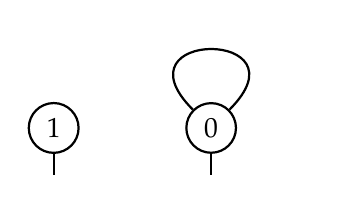
\begin{tikzpicture}[scale=1, transform shape, every loop/.style={}]
    \node[circle,draw=black,thick] (B) at (-1,0) {$1$};
    \draw[-,thick] (B) -- (-1,-0.6);
    \node[circle,draw=black,thick] (A) at (1,0) {$0$};
    \draw[-,thick] (A) -- (1,-0.6);
    \path[every node/.style={font=\sffamily\small},thick]
        (A)   edge[loop] (A);
    \end{tikzpicture}
    \end{center}
    \caption{$g=1, n=1$的稳定图}%
    \label{fig:03graphloop}
    \end{figure}
    第一个图$\Gamma_1$给出贡献
    \begin{align*}
        \Cont_{\Gamma_1} &= T\omega_{1,1}^{\E}(R(z)^{-1}\1) \\
        &= \omega_{1,1}^{\E}(R(z)^{-1}\1) + p_* \omega_{1,1}^{\E}(R(z)^{-1}\1, T_R(z)).
    \end{align*}
    利用公式$B_2 = \frac{1}{6}$以及$\dim \Mbar_{1,1} = 1$这一事实，它成为
    \[ 1 - \frac{1}{12}\psi_1 + \frac{1}{12} \kappa_1. \]
    第二个图没有尾部贡献，因为$\dim \Mbar_{0,3} = 0$。边贡献的常数项是$\frac{1}{12}$，所以考虑自同构并推前到$\Mbar_{1,1}$给出
    \[ \Cont_{\Gamma_2} = \frac{1}{12} \Delta, \]
    其中$\Delta$表示边界除子（带正确的叠结构）。由于此时$\psi_1 = \kappa_1$，我们得到
    \[ 1+\lambda_1 = 1 + \frac{1}{12}(\kappa_1 - \psi_1 + \Delta) = 1 + \frac{1}{12} \Delta. \]
\end{exm}




\subsection{算子形式体系与几何量子化}%
\label{sub:Operator formalism and geometric quantization}

我们回到 Givental 的辛形式体系。它对某些计算更为方便，但实际上与我们之前的东西是相同的，至少在我们想计算生成函数时如此。回忆我们在$V$上有 Frobenius 流形结构，并且考虑了向量空间$\mc{V}\coloneqq V\ls{z^{-1}}$，带辛形式
\[ (\mbf{f}(z), \mbf{g}(z)) \coloneqq \on{Res}_{z=0} \eta(\mbf{f}(-z), \mbf{g}(z)). \]
若我们考虑由$\mc{V}_+ = V[z]$和$\mc{V}_- = z^{-1}V\ps{z^{-1}}$给出的极化，那么令$\bq$如前（带膨胀子平移），并令$\bp$为$\mc{V}_-$上的坐标，使得$(\bq, \bp)$构成$\mc{V}$的一组 Darboux 坐标系。

\begin{defn}
    我们把任何形如
    \[ \mc{D} = \exp\ab(\sum_{g=0}^{\infty} \hbar^{g-1} \mc{F}_g) \]
    的形式函数称为 \textit{Fock 空间的渐近元}。
\end{defn}

然后给定这样一个 Fock 空间的渐近元，我们通过如下公式量子化$\mc{V}$上的（无穷小）辛变换：
\[ \wh{p_a p_b} \coloneqq \hbar \partial_{q_a} \partial_{q_b}, \qquad \wh{p_a q_b} \coloneqq q_b \partial_{q_a}, \qquad \wh{q_a q_b} = \frac{q_a q_b}{\hbar}. \]
特别地，这将使我们能理解像$\hat{R} \mc{D}$这样的表达式。然而，我们需要小心，因为我们的公式将同时涉及基本解$S_{\tau}$和$R$-矩阵，而$S_{\tau}$是关于$z^{-1}$的幂级数。\footnote{这是因为我们把$\frac{1}{z-\psi} = \sum_{n=0}^{\infty} \psi^n z^{-n-1}$展开。}

\begin{thm}[Givental {\cite{Givental2001quantization}}]
    形如$S(z^{-1}) = \mr{Id} + S_1 z^{-1} + \cdots$的算子通过公式
    \[ \hat{S}^{-1} \mc{D}(\bq) = e^{\frac{1}{2\hbar}W(\bq,\bq)} \mc{D}([S \bq]_+), \]
    作用在 Fock 空间的（渐近）元上，其中$W = \sum \eta(W_{mn}q_m, q_n)$由公式
    \[ \frac{S(w^{-1})^* S(z^{-1}) - \mr{Id}}{w^{-1}+z^{-1}} = \sum \frac{W_{mn}}{w^m z^n}. \]
    定义。形如$R(z) = \mr{Id} + R_1 z + \cdots$的算子通过公式
    \[ \hat{R}\mc{D}(\bq) = e^{\frac{\hbar}{2} V(\partial_{\bq}, \partial_{\bq})} \mc{D}(R^{-1} \bq), \]
    作用，其中$V = \sum \eta(p_m, V_{mn} p_n)$由
    \[ \frac{R(w)^* R(z) - \mr{Id}}{w+z} = \sum V_{mn} w^m z^n. \]
    定义。
\end{thm}

对半单 CohFT，存在一组\textit{典范坐标}$u_{\alpha}$，使得$1$-形式$\d{u}$是代数同态$T_v V \to \C$。那么在半单点附近，量子联络有形如
\[ \Psi \cdot  R \cdot e^{\frac{U}{z}}, \]
的渐近解，其中$\Psi$把平坦坐标转换为典范坐标，$U = \on{diag}(u_{\alpha})$是典范坐标的矩阵。最后，定义
\[ C = \frac{1}{2} \int^u \sum R_1^{\alpha\alpha} \d{u_{\alpha}}. \]
Teleman 重构定理的一个推论是公式
\[ \mc{D}^X = e^{C(u)} \hat{S}^{-1}_{\tau} \hat{\Psi} \hat{R} \wh{e^{\frac{U}{z}}} \prod_{i=1}^{\dim V} \mc{D}^{\mr{pt}} \]
它对任何具有半单量子上同调的光滑射影簇的 Gromov-Witten 理论成立。

\begin{exm}
    作为最后一个例子，我们将应用 Teleman 定理来计算任意半单 CohFT 的$F_1$。设$e_{\mu}$表示量子乘积的幂等基。我们来计算
    \[ \int_{\Mbar_{1,1}} \Omega_{1,1}(e_{\beta}). \]
    利用重构定理，我们得到
    \begin{align*}
        \int_{\Mbar_{1,1}}\Omega_{1,1}(e_{\beta}) ={}& \int_{\Mbar_{1,1}} T_R \omega_{1,1}(R(\bar{\psi})^{-1} e_{\beta}) + \frac{1}{2} T_R \omega_{0,3}(R(\bar{\psi})^{-1} e_{\beta}, V(\bar{\psi}_2, \bar{\psi}_3)) \\
        ={}& \int_{\Mbar_{1,1}}T_R\omega_{1,1}(e_{\beta}) - \int_{\Mbar_{1,1}} T_R \omega_{1,1}(R_1 e_{\beta})\bar{\psi} \\
        &+ \frac{1}{2}\sum_{\mu}  \omega_{0,3}(e_{\beta}, R_1 e^{\mu}, e_{\mu}) \\
        ={}& \int_{\Mbar_{1,1}} ( \omega_{1,1}(e_{\beta}) + p_* ( \omega_{1,2}(e_{\beta}, R_1 \1) \bar{\psi}_2^2 )) \\
        &- \int_{\Mbar_{1,1}} (\omega_{1,1}(R_1 e_{\beta})\bar{\psi}_1 + p_* ( \omega_{1,2}(R_1 e_{\beta}) \bar{\psi}_2^2 ) \bar{\psi}_1) \\
        &+ \frac{1}{2} \sum_{\mu} \eta(e_{\beta} \star e_{\mu}, R_1 e^{\mu}) \\
        ={}& \frac{1}{24} \sum_{\mu} ( \omega_{0,4}(e_{\mu}, e^{\mu}, e_{\beta}, R_1 \1) -\omega_{0,3}(e_{\mu}, e^{\mu}, R_1 e_{\beta}) )\\
        &+ \frac{1}{2} \eta(e_{\beta}, R_1 e^{\beta}) \\
        ={}& \frac{1}{24} \sum_{\mu}\sum_{\nu} \omega_{0,3}(e_{\mu}, e^{\mu}, e_{\nu})\omega_{0,3}(e^{\nu}, e_{\beta}, R_1 \1) \\
        &-\frac{1}{24} \sum_{\mu} \omega_{0,3}(e_{\mu}, e^{\mu}, R_1 e_{\beta}) + \frac{1}{2} (R_1)_{\beta\beta} \\
        ={}& \frac{1}{24} \ab(\eta(e^{\beta}, R_1 \1) - \sum_{\mu} \eta(e^{\mu}, R_1 e_{\beta})) + \frac{1}{2} (R_1)_{\beta\beta}.
    \end{align*}
    利用恒等式
    \begin{align*}
        \eta(R_1 \1, e^{\beta}) - \sum_{\mu} \eta(R_1 e_{\beta}, e^{\mu}) &= \sum_{\mu} \Delta_{\mu} \int_{\Mbar_{0,4}} \Omega_{0,4}(e_{\mu}, e_{\mu}, e_{\mu}, e_{\beta}) \\
        &= -\frac{1}{2}\sum_{\mu} \Delta_{\mu} \partial_{u_{\beta}} \Delta_{\mu}^{-1} \\
        &= \frac{1}{2} \sum_{\mu} \partial_{u_{\beta}} \log \Delta_{\mu},
    \end{align*}
    其中$\Delta_{\mu} \coloneqq \eta(e_{\mu}, e_{\mu})^{-1}$，我们得到结果
    \[ \int_{\Mbar_{1,1}} \Omega_{1,1}(e_{\beta}) = \frac{1}{48} \sum_{\mu} \partial_{u_{\beta}} \log \Delta_{\mu} + \frac{1}{2} (R_1)_{\beta\beta}, \]
    它可以写成如下富有启发性的形式
    \[ \d{F_1^{\Omega}} = \sum_{\mu} \ab( \frac{\d{\log \Delta_{\mu}}}{48} + \frac{1}{2} (R_1)_{\mu\mu} \d{u_{\mu}} ). \]
    这恢复了 Givental 早已知道的一个结果。
\end{exm}

\subsection{如何计算 R-矩阵}%
\label{sub:How to compute the R-matrix}

最后我们来解释如何计算 R-矩阵，先从 Frobenius 流形是共形的情形开始（例如光滑射影簇的 Gromov-Witten 理论、\(r\)-旋量曲线等）。在这个例子中，我们按照~\cite{PPZ2015}考虑 3-旋量曲线的 Frobenius 流形。设\(V\)是 2 维的，坐标为\(x\)和\(y\)，其中\(x\)对应单位。度量由
\[ \eta = \begin{pmatrix}
    0 & 1 \\
    1 & 0
\end{pmatrix} \]
给出，初级亏格零势为\(F(x,y) = \frac{1}{2} x^2 y + \frac{1}{72} y^4\)。存在 \textit{Euler 向量场}
\[ E = x \pdv{}{x} + \frac{2}{3} y \pdv{}{y}, \]
它分别以权\(-1\)和\(-\frac{2}{3}\)作用在\(\partial_x\)和\(\partial_y\)上。共形维数是\(\delta = \frac{1}{3}\)，我们定义次数算子
\[ \mu(v) = [E,v] + \ab(1 - \frac{\delta}{2})v. \]
这里\(\partial_x\)的次数为\(-\frac{1}{6}\)，\(\partial_y\)的次数为\(\frac{1}{6}\)。

为了简化起见，我们令\(\phi = \frac{y}{3}\)并定义
\[ \hat{\partial}_x = \phi^{1/4} \partial_x, \qquad \hat{\partial}_y = \phi^{-1/4} \partial_y, \]
然后在这个标架下计算。在此设定下，量子乘法由
\[ \hat{\partial}_x \star \hat{\partial}_x = \phi^{1/4} \hat{\partial}_x, \qquad \hat{\partial}_x \star \hat{\partial}_y = \phi^{1/4} \hat{\partial}_y, \qquad \hat{\partial}_y \star \hat{\partial}_y = \phi^{1/4} \hat{\partial}_x. \]
给出。我们最后需要的是，与\(E\)的量子乘法由
\[ E \star - = \begin{pmatrix}
    x & 2 \phi^{3/2} \\
    2 \phi^{3/2} & x
\end{pmatrix}. \]
给出。现在我们利用递归方程
\[ [R_{k+1}, E \star -] = (k + \mu) R_k. \]
来计算 R-矩阵\(R = 1 + R_1 z + \cdots\)。令\(R_k = \begin{psmallmatrix}
    a_k & b_k \\
    c_k & d_k
\end{psmallmatrix}\)，我们得到方程
\[ \ab[
    \begin{pmatrix}
        a_{k+1} & b_{k+1} \\
        c_{k+1} & d_{k+1}
    \end{pmatrix}, \begin{pmatrix}
        x & 2 \phi^{3/2} \\
        2 \phi^{3/2} & x
    \end{pmatrix}
] = \frac{1}{6} \pdiagmat[empty={}]{6k-1, 6k+1} \begin{pmatrix}
    a_k & b_k \\
    c_k & d_k
\end{pmatrix}. \]

它的唯一解事实上是
\begin{align*}
    a_k &= \frac{1}{1728^k \phi^{3k/2}} \frac{1+6k}{1-6k} \frac{(6k)!}{(3k)!(2k)!} \delta_{k, \text{偶}},  \\
    b_k &= \frac{1}{1728^k \phi^{3k/2}} \frac{1+6k}{1-6k}\frac{(6k)!}{(3k)!(2k)!} \delta_{k, \text{奇}},  \\
    c_k &= \frac{1}{1728^k \phi^{3k/2}}\frac{(6k)!}{(3k)!(2k)!} \delta_{k, \text{奇}}, \\
    d_k &= \frac{1}{1728^k \phi^{3k/2}} \frac{(6k)!}{(3k)!(2k)!} \delta_{k, \text{偶}}.
\end{align*}
如果你熟悉曲线模空间上的重言关系，你会看到级数\(a_k + b_k\)和\(c_k + d_k\)出现在 Faber-Zagier 关系和 Pixton 关系的表述中。

在 Frobenius 流形非共形的情形（例如等变 Gromov-Witten 理论），我们需要用振荡积分或其他技术来确定 R-矩阵的初值。这里我们给出一个例子计算，它归功于 Givental~\cite{Givental2001semisimple}。在此设定下，\(X = \P^n\)，但论证对任何 Fano 环面簇都可行。回忆\(\P^n\)的等变镜像是超势
\[ W = x_1 + \cdots + x_{n+1} + \sum_{i=1}^{n+1} \lambda_i \log x_i \]
（这里为方便起见我们改变了等变参数的符号）。因此，振荡积分形如
\[ I = \int_{\Gamma \subset E_q = (x_1 \cdots x_{n+1}=q)} e^{W/z} \prod_{i=1}^{n+1} \frac{\d{x_i}}{x_i}. \]
它被算子
\[ \prod_{i=1}^{n+1}\ab(zq \odv{}{q} -\lambda_i) - q, \]
零化，这恰好是射影空间 I-函数所满足的 Picard-Fuchs 方程。

为了在临界点附近展开这个积分，我们首先需要计算临界点。这里，使用坐标\(t = \log q\)和\(T_i = \log x_i\)，我们得到方程
\[ x_i = L - \lambda_i, \]
其中\(L\)是 Lagrange 乘子。它们满足方程
\[ \prod_{i=1}^{n+1} (L - \lambda_i) = q, \]
因此对一般的\(\lambda\)值，在\(q = 0\)附近，Lagrange 乘子的可能取值\(L_i\)由它们以哪个\(\lambda_i\)开头来区分。注意函数\(W\)、Lagrange 乘子的值、从而临界点，都连续依赖于\(\lambda\)，所以当\(q \neq 0\)时它们在\(\lambda = 0\)处有非等变极限。

当\(q = 0\)时，矩阵\(\Psi\)把平坦基\(\ab{H^i}\)转换到基
\[ L_i(H) = \prod_{j \neq i} \frac{H - \lambda_j}{(\lambda_i - \lambda_j)^{1/2}}, \]
它们是典范坐标的首项（只需通过等变局部化计算环面作用的不动点，我们就得到这个 Lagrange 插值）。因此，我们需要在\(q = 0\)极限下计算\(L_j \ab(z q \odv{}{q}) I\)。直接计算表明，把\(L_i \ab(z q \odv{}{q})\)作用在积分上会给振荡积分的被积函数引入一个正比于\(\frac{q}{x_i}\)的额外因子。由于我们可以置换指标，我们只计算\(i = n+1\)的情形。另一个直接计算表明，除非\( j = n+1\)，否则积分在\(q = 0\)处为零，所以事实上我们看到\(R\)在经典极限下是对角的。当\(j = n+1\)时，我们有
\[ \frac{q}{x_{n+1}} = x_1 \cdots x_n, \]
积分成为
\[ \int_{\Gamma} e^{\ab( \sum_{i=1}^n x_i + (\lambda_i - \lambda_{n+1})\log x_i ) / z} \d{x_1} \cdots \d{x_n} = \prod_{i=1}^n \int_{\R} e^{x_i/z} x_i^{(\lambda_i - \lambda_{n+1})/z} \d{x_i}, \]
这不过是 Γ-函数的乘积。

\begin{lem}
    我们有渐近式
    \[ \log \Gamma(1+s) \sim s \log \ab(\frac{s}{e}) + \frac{1}{2} \log(2\pi s) + \sum_{k=1}^{\infty} \frac{B_{2k}}{2k} \frac{s^{1-2k}}{2k-1}. \]
\end{lem}
利用这一点，我们看到在\(q = 0\)处，R-矩阵的对角矩阵元由
\[ \log R = \sum_{k=1}^{\infty} \frac{B_{2k}}{2k} \frac{z^{2k-1}}{2k-1} \sum_{i =1}^n (\lambda_i - \lambda_{n+1})^{1-2k}. \]
给出。由 Givental 的一个结果，这蕴含该 R-矩阵恢复了\(\P^n\)的等变 GW 理论；作为推论，由于非等变极限存在，我们得到\(\P^n\)的 Virasoro 约束。


\section{半小映射的分解定理（文学清）}%
\label{sec:Decomposition theorem for semi-small maps (Xueqing Wen)}

\begin{quest}
    设\(X\)是一个（流形、簇、解析空间等）。我们如何计算\(H^*(X, \C)\)？
\end{quest}

不幸的是，这个问题太难了，所以我们用一个新的问题来代替它。

\begin{quest}
    我们如何利用更小的空间来探测\(H^*(X, \C)\)？
\end{quest}

\begin{thm}[K\"unneth 公式]
    我们有\(H^*(X \times Y, \C) = H^*(X, \C) \otimes H^*(Y, \C)\)。
\end{thm}

不幸的是，大多数空间都不是乘积，所以我们考虑如下问题。

\begin{quest}
    设\(f \colon X \to Y\)是一个态射。我们能否利用\(Y\)的上同调以及\(f\)的纤维的上同调来探测\(X\)的上同调？
\end{quest}

这个问题仍然非常困难，但至少我们可以研究它。我们从\(f\)是紧流形之间的纤维丛的情形开始。答案当然是 Leray 或 Serre 谱序列，但在此之前，我们需要一些预备知识。

\begin{defn}
    \(Y\)上的一个\(\ul{\C}_Y\)-局部系统是\(Y\)上的一个由向量空间构成的局部常值层\(\mc{L}\)。
\end{defn}

例如，若\(Y\)连通，则局部系统对应于\(\pi_1(Y)\)的表示。另外注意，若\(Y\)是代数簇，我们需要使用它的解析化。

\begin{exm}
    设\(f\)是如上所述的以\(F\)为纤维的纤维丛。则\(R^i f_* \ul{\C}_X\)是\(Y\)上以\(H^i(F, \C)\)为纤维的局部系统。
\end{exm}

\begin{prop}
    我们有
    \[ H^*(X, \C) = H^*(X, \ul{\C}_X) = H^*(\mr{pt}, R a_{X*} \ul{\C}_X). \]
\end{prop}

\begin{thm}[Leray/Serre 谱序列]
    我们有谱序列
    \[ E_2^{p,q} = H^p(Y, R^q f_* \ul{\C}_X) \Rightarrow H^{p+q}(X, \C). \]
\end{thm}

现在我们考虑\(f \colon X \to Y\)是光滑射影簇之间的光滑射影映射的情形。

\begin{thm}[Deligne {\cite{Deligne1968}}]
    我们有非典范同构
    \[ R f_* \ul{\C}_X = \bigoplus_{q \geq 0} R^q f_* \ul{\C}[-q]. \]
    在上同调的层面，我们有
    \[ H^*(X, \C) = \bigoplus_{q \geq 0} H^{*-q}(Y, R^q f_* \ul{\C}). \]
\end{thm}

这是射影簇的硬 Lefschetz 定理的推论，它也表明 Serre 谱序列在\(E_2\)页退化。在拓扑中，这对 Hopf 纤维化不成立。

现在我们考虑\(f \colon X \to Y\)是代数簇之间的紧合映射的情形。此时我们有一个 \textit{Whitney 分层}\footnote{我们明确拒绝定义它。}\(Y = \bigsqcup_{\lambda} Y_{\lambda}\)，使得\(f^{-1}(Y_{\lambda}) \to Y_{\lambda}\)是一个以（可能奇异的）簇为纤维的\(C^{\infty}\)纤维化。

\begin{defn}
    \(Y\)上的一个\(\ul{\C}_Y\)-模\(\mc{F}\)称为\textit{可构造层}，如果存在 Whitney 分层\(Y = \bigsqcup Y_{\lambda}\)使得对所有\(\lambda\)，\(\mc{F}|_{Y_{\lambda}}\)是局部系统。
\end{defn}

有了这个定义，我们可以考虑\(Y\)上可构造层的导出范畴\(\mc{D}_c^b(Y)\)。这一构造具有六函子形式体系，其中的函子为\(f_*, f^*, f_!, f^!, \otimes, \mc{H}\mr{om}\)，并且通过函子
\[ D_Y \colon \mc{D}_c^b(Y) \to \mc{D}_c^b(Y) \]
满足 Verdier 对偶。

\begin{defn}
    复形\(\mc{F}^{\bullet} \in \mc{D}_c^b(Y)\)称为\textit{反常层}，如果它满足如下条件：
    \begin{enumerate}
        \item （支集条件）对所有\(i\)，我们有\(\dim \on{supp} \mc{H}^{-i}(\mc{F}^{\bullet}) \leq i\)；
        \item （余支集条件）对所有\(i\)，我们有\(\dim \on{supp} \mc{H}^{-i}(D_Y \mc{F}^{\bullet}) \leq i\)。
    \end{enumerate}
\end{defn}

\begin{rmks}\leavevmode
    \begin{enumerate}
        \item 反常层并不是层，而是集中在次数\([-\dim Y, 0]\)中的复形。
        \item 它们有两个来源。一个是相交同调，另一个是 Riemann-Hilbert 对应。
    \end{enumerate}
\end{rmks}

我们需要用到如下事实：\(Y\)上反常层的范畴\(\ms{Perv}(Y)\)是一个 Abel 范畴，并且还是\(\mc{D}_c^b(Y)\)上某个\(t\)-结构的心。特别地，对任意\(\mc{G} \in \mc{D}_c^b (Y)\)，我们可以考虑反常上同调\(^p\mc{H}^i(\mc{G}) \in \ms{Perv}(Y)\)。

\begin{thm}[Beilinson-Bernstein-Deligne-Gabber {\cite{BBD1982}}]
    设\(f \colon X \to Y\)是代数簇之间的紧合态射。假设\(X\)光滑且连通。\footnote{这不是必需的，但若去掉光滑性假设，我们需要考虑相交复形。}则
    \[ R f_* \ul{\C}_X [\dim X] = \bigoplus_{i} {^p\mc{H}^i}(R f_* \ul{\C}_X)[-i]. \]
    此外，每个\(^p\mc{H}^i (R f_* \ul{\C}_X)\)都是半单的（即每个子对象都是直和项）。
\end{thm}

\begin{defn}
    设\(f \colon X \to Y\)是紧合满态射，其中\(X\)光滑且不可约。设\(Y = \bigsqcup Y_{\lambda}\)是一个分层，使得\(f^{-1}(Y_{\lambda}) \to Y_{\lambda}\)是\(C^{\infty}\)-纤维化。我们称\(f\)是\textit{半小}的，如果对所有\(y_{\lambda} \in Y_{\lambda}\)，我们有\(\on{codim}_Y Y_{\lambda} \geq 2 \dim f^{-1} (y_{\lambda})\)。若等号成立，我们称\(Y_{\lambda}\)是\textit{相关}的。若唯一的相关层是稠密的那个层，则我们称\(f\)是\textit{小}的。
\end{defn}

\begin{thm}[{\cite{DeCataldoMigliorini2002}}]
    若\(f \colon X \to Y\)是半小的，则\(R f_* \ul{\C}_X [\dim X]\)是\(Y\)上的反常层。
\end{thm}

\begin{proof}
    对\(y_{\lambda} \in Y_{\lambda} \subseteq Y\)，我们看到
    \[ R f_* \ul{\C}_X |_{y_{\lambda}} = \bigoplus H^i (f^{-1}(y_{\lambda}), \C). \]
    注意当\(i > 2 \dim f^{-1}(y_{\lambda}) \leq \on{codim}_Y (Y_{\lambda})\)时它为零。让\(Y_{\lambda}\)取遍所有层，我们便得到支集条件。由于\(f\)紧合，我们有\(R f_* = f_!\)，再利用\(D_Y R f_* = f_! D_X\)，我们便得到余支集条件。
\end{proof}

\begin{exms}
    我们现在给出一些半小映射的例子。
    \begin{enumerate}
        \item 曲面之间任意一般有限的紧合映射都是半小的。
        \item 设\(Y = \ab\{xy = t^{\ell+1}\} \subseteq \C^3\)。则存在奇点的平凡典范消解\(f \colon \tilde{Y} \to Y\)，且奇点上方的纤维是一串\(\P^1\)构成的链，所以它是半小的（另见前一个例子）。
    \end{enumerate}
\end{exms}

\begin{thm}[Kaledin {\cite{Kaledin2006}}]
    从非奇异全纯辛簇出发的射影双有理映射是半小的。
\end{thm}

\begin{exm}
    例如，Springer 消解与 Grothendieck-Springer 消解是半小的。此外，曲面上点的 Hilbert 概形的 Hilbert-Chow 态射也是半小的。
\end{exm}

设\(f \colon X \to Y\)是半小的，并考虑分层\(Y = \bigsqcup Y_{\lambda}\)。若\(Y_{\lambda}\)是相关的，考虑
\[ \mc{L}_{\lambda} = R^{d_{\lambda}} f_* \ul{\C}_{f^{-1}(Y_{\lambda})}, \]
其中\(d_{\lambda} = 2 \dim f^{-1} (y_{\lambda})\)。则\(\mc{L}_{\lambda}\)是半单的。这里注意\(\mc{L}_{|\lambda} = H^{d_{\lambda}}(f^{-1}(y_{\lambda}), \C)\)。现在令\(\mr{IC}(\mc{L}_{\lambda})\)为\(\mc{L}_{\lambda}[\dim Y_{\lambda}]\)在\(\ol{Y}_{\lambda}\)上的中间扩张，它是一个反常层。

\begin{thm}[{\cite{DeCataldoMigliorini2002}}]
    设\(f \colon X \to Y = \bigsqcup Y_{\lambda}\)是半小的。则存在典范分解
    \[ R f_* \ul{\C}_X[\dim X] = \bigoplus_{Y_{\lambda}\text{相关}} \mr{IC}(\mc{L}_{\lambda}). \]
\end{thm}

\begin{exm}
    设\(G\)是约化群，其 Lie 代数为\(\g\)，并选取一个 Borel 子群\(B\)。则
    \[ G \times_B \b = \tilde{\g} \xrightarrow{\pi} \g \]
    是小的。因此，我们有
    \[ R \pi_* \ul{\C}_{\tilde{\g}} [\dim \g] = \mr{IC}(\mc{L}). \]
    回忆\(\tilde{\g}^{\on{rs}} \to \g^{\on{rs}}\)是一个\(W\)-挠子。则对\(a \in \g^{\on{rs}}\)，我们有\(\mc{L}_{|a} \cong \C[W]\)，从而\(\mc{L} = R^0 \pi_* \ul{\C}_{\tilde{\g}^{\on{rs}}}\)。这意味着\(W\)作用在\(\mc{L}\)上，且这一作用可以延拓到\(\mr{IC}(\mc{L})\)上以及\(R \pi_* \C_{\tilde{\g}}\)上，特别地，对任意\(a \in \g\)，它作用在纤维\(R \pi_* \C_{\tilde{\g}}|_a\)上。
\end{exm}

\begin{exm}
    考虑 Springer 消解\(\mu \colon T^*(\on{GL}_3/B) \to \mc{N} = \mathbb{O}_{(1^3)} \sqcup \mathbb{O}_{(2,1)} \sqcup \mathbb{O}_{(3)}\)。这个映射是半小的，但不幸的是所有幂零轨道都是相关的。注意\((2,1)\)轨道上方的纤维是两条\(\P^1\)在一个结点处粘合而成的并，\((3)\)轨道上方的纤维是一个点，而\((1^3)\)轨道上方的纤维是\(\on{GL}_3/B\)。

    我们看到\(\mc{L}_{(3)}\)必定是平凡的，因为\(\mu\)在这个轨道上方是同构。然后\(\mc{L}_{(2,1)} = R^2 \mu_* \ul{\C}\)是\(\mathbb{O}_{(2,1)}\)上的秩\(2\)局部系统。最后，\(\mc{L}_{(1^3)} = R^6 \mu_* \ul{\C}\)是\(\mathbb{O}_{(1^3)} = \mr{pt}\)上的秩\(1\)局部系统。因此，我们有
    \[ R \mu_* \ul{\C}_{T^*\on{GL}_3/B}[6] = \mr{IC}(\mc{L}_{(3)}) \oplus \mr{IC}(\mc{L}_{(2,1)}) \oplus \mr{IC}(\mc{L}_{(1^3)}). \]
    限制到\(b \in \mathbb{O}_{(3)}\)，我们得到\(\mc{L}_{(3)} = H^0(\mr{pt})\)。限制到\(a \in \mathbb{O}_{(2,1)}\)，我们得到
    \[ H^0(X, \C) \oplus H^2(X, \C) = \mr{IC}(\mc{L}_{(3)})|_{(a)} \oplus \mr{IC}(\mc{L}_{(2,1)})|_{(a)}. \]
    限制到\(0 = \mathbb{O}_{(1^3)}\)，我们得到
    \begin{align*}
        H^*(\on{GL}_3/B, \C) = \C[W] &= \mr{IC}(\mc{L}_{(3)})|_0 \oplus \mr{IC}(\mc{L}_{(2,1)})|_0 \oplus \mc{L}_{(1^3)}|_0 \\
        &= H^0(\on{GL}_3/B, \C) \oplus \ab(\text{一个维数为 } 4 \text{ 的直和项}) \oplus H^6(\on{GL}_3/B, \C).
    \end{align*}
    作为\(W = S_3\)的表示，它们分别对应于平凡表示、标准表示的两个副本以及符号表示。关于 Springer 理论的构造以及这些分解，参见~\cite{BorhoMacPherson1983}。
\end{exm}


\section{量子 K-理论（阎霄汉、周祐正）}%
\label{sec:Quantum K-theory (Xiaohan Yan and You-Cheng Chou)}

\subsection{概述}%
\label{sub:Overview}

Gromov-Witten 不变量是“计数”光滑射影簇\(X\)中曲线的一种方式。GW 理论给出形如
\[ \ab<\alpha_1, \ldots, \alpha_n>_{g, n, \beta} \in \Q \]
的数，其中\(\alpha_i \in H^*(X)\)是各种类，\(g\)是亏格，\(n\)是标记点的个数，\(\beta \in H_2(X, \Z)\)是曲线类。它被用来研究镜像对称，而在镜像对称之外也给出了双有理不变量。我们现在的目标是把这整套理论提升到 K-理论。量子 K-理论给出数
\[ \ab<V_1, \ldots, V_n>_{g, n, \beta} \in \Z \]
其中\(V_1, \ldots, V_n \in K(X)\)。它们满足各种差分方程\footnote{对比上同调中的微分方程。}，并且在三维镜像对称和表示论中有各种应用。

\subsection{K-理论}%
\label{sub:K-theory}

\begin{defn}
    设\(X\)为光滑射影簇。则\(X\)的\textit{K-理论}\(K(X)\)是\(X\)上向量丛的 Grothendieck 群，其关系为：若
    \[ 0 \to V_1 \to V_2 \to V_3 \to 0 \]
    是短正合列，则\(V_2 = V_1 + V_3\)。
\end{defn}

\begin{rmk}\leavevmode
    \begin{enumerate}
        \item 在直和与张量积运算下，\(K(X)\)是一个环；
        \item 至少在\(\Q\)上，陈特征给出同构\(K(X) \to A^*(X)\)。
    \end{enumerate}
\end{rmk}

\begin{exm}
    设\(X = \P^n\)，并令\(P = \mc{O}(-1)\)。则我们有
    \[ K(X) = \C[P^{\pm 1}]/(P-1)^{n+1} \xrightarrow{\on{ch}} A^*(X) = \C[H]/H^{n+1}. \]
\end{exm}

对于不假设光滑的 Deligne-Mumford 叠，有两个版本
\[ K_0(X) \supset K^0(X), \]
其中\(K_0\)指凝聚层，\(K^0\)指完美复形。在光滑射影簇上二者一致，因此从现在起\(K(X)\)将指\(K_0(X)\)。有张量积
\[ K^0(X) \otimes K_0(X) \to K_0(X) \]
以及推前
\[ f_* \colon K(X) \to K(Y) \qquad V \mapsto \sum (-1)^i R^i f_* V \]
沿紧合态射。若\(f\)是完美态射（例如平坦、正则嵌入等），则有拉回
\[ f^* \colon K(Y) \to K(X) \qquad W \mapsto \sum (-1)^i \on{Tor}_i^{f^{-1} \mc{O}_Y} (\mc{O}_X, f^{-1} W). \]

\subsection{曲线的模}%
\label{sub:Moduli of curves}

回忆模空间
\[ \bar{M}_{g,n}(X, \beta) = \ab\{ f \colon (\Sigma, p_1, \ldots, p_n) \to X \mid g(\Sigma) = g, f_*[\Sigma] = \beta, \abs{\Aut f} < \infty \} \]
，即到\(X\)的稳定映射的模空间。它有赋值映射
\[ \ev_i \colon \bar{M}_{g,n}(X, \beta) \to X \qquad (f, \Sigma, \ul{p}) \mapsto f(p_i). \]
还有泛余切线\(L_i = \sigma_i^* \omega_{ \mc{C}/\bar{M} }\)。

该模空间是一个紧合 DM 叠，带有完美障碍理论，从而给出虚结构层\(\mc{O}^{\vir}_{g,n,\beta}\)。这来自\textit{虚切丛}的结构，其中
\[ \mathbb{T}_{(f, \Sigma, \ul{p})} \bar{M}_{g,n}(X, \beta) = \chi(\Sigma, f^* T_X) - \chi(\Sigma, T_{\Sigma}(-p_1 - \cdots - p_n)). \]
粗略地说，若\(\bar{M}\)是簇\(Y\)上向量丛\(E\)的某个截面的零点轨迹，则\(\mc{O}^{\vir} = \mc{O}_Y \otimes \mr{Eu}(E)\)，其中 K-理论欧拉类为\(\mr{Eu}(E) = \sum (-1)^i \Lambda^i E^{\vee}\)。

\subsection{KGW 不变量}%
\label{sub:KGW invariants}

关于量子 K-理论，参见~\cite{Lee2004}；关于置换等变理论，参见~\cite{Givental2017K1,GiventalK7}。下面用到的 Deligne-Mumford 叠的 Riemann-Roch 公式由 To\"en~\cite{Toen1999}证明。

\begin{defn}
    K-理论 GW 不变量定义为
    \[ \ab<V_1, \ldots, V_n>_{g,n,\beta} \coloneqq \chi\ab(\bar{M}_{g,n}(X, \beta); \mc{O}^{\vir} \otimes \bigotimes_{i=1}^n \ev_i^* V_i). \]
\end{defn}

若\(V_1, \ldots, V_n\)是真正的向量丛，则该不变量是整数，但一般地我们将考虑系数在特征零域中的\(K_0\)。我们也可以定义引力后代
\[ \ab<V_1 L_1^{k_1}, \ldots, V_n L_n^{k_n}>_{g,n,\beta} \coloneqq \chi\ab(\bar{M}_{g,n}(X, \beta); \mc{O}^{\vir} \otimes \bigotimes_{i=1}^n ( \ev_i^* V_i )L_i^{k_i} ). \]
利用\(S_n\)通过置换标记点在\(\bar{M}_{g,n}(X, \beta)\)上的作用，对象\(\bigotimes_{i=1}^n \ev_i^* V\)与\(\bigotimes_{i=1}^n L_i^k\)是\(S_n\)-等变的。

\begin{defn}
    我们定义\textit{置换不变 K-理论 GW 不变量}为
    \begin{align*}
        \ab<V L_1^k, \ldots, V L_n^k>_{g,n,\beta}^{S_n} &\coloneqq \chi\ab([ \bar{M}_{g,n}(X, \beta)/S_n ]; \mc{O}^{\vir} \otimes \bigotimes_{i=1}^n ( \ev_i^* V ) L_i^k) \\
        &= \dim \chi_{S_n} \ab(\bar{M}_{g,n}(X, \beta); \mc{O}^{\vir} \otimes \bigotimes_{i=1}^n ( \ev_i^* V ) L_i^k )^{S_n}.
    \end{align*}
\end{defn}

给定\(t(q) = \sum_{n \in \Z} t_n q^n \in K(X)[q,q^{-1}]\)，我们可以定义
\[ \ab< t(L_1), \ldots, t(L_n)>^{S_n}_{g,n,\beta} \coloneqq \chi ([\bar{M}_{g,n}(X,\beta)/S_n], \cdots). \]
更一般地，若\(H = S_{a_1} \times \cdots \times S_{a_m} \subset S_n\)，我们可以定义
\[ \ab<t_1(L_1), \ldots, t_1(L_{a_1}), t_2(L_{a_1+1}), \ldots, t_2(L_{a_1+a_2}), \ldots>_{g,n,\beta}^H. \]

\begin{rmk}
    我们想讨论一下与通常 GW 不变量的关系。回忆 Hirzebruch-Riemann-Roch 定理说
    \[ \chi(M; V) = \int_M \on{ch}(V) \on{td}(T_M). \]
    当\(M\)是光滑 DM 叠时，T\"oen 证明了公式
    \[ \chi(M; V) = \int_{IM} \wt{\on{ch}}(V) \wt{\on{td}}(T_M), \]
    其中\(IM = M \times_{\Delta, M \times M, \Delta} M\)是\(M\)的惯性叠，波浪号表示取轨形陈特征与 Todd 类。
\end{rmk}

\begin{exm}
    若\(M = B\mu_r\)，则\(IM = \bigsqcup_{g \in \mu_r} B \mu_r\)。若\(M = \P(1, r)\)是加权\(\P^1\)，则\(IM = M \sqcup \bigsqcup_{g \neq 1 \in \mu_r} B\mu_r\)。
\end{exm}

\begin{exm}
    设\(M = BG\)，其中\(G\)是有限交换群，并设\(V\)是\(BG\)上的向量丛，这等同于\(G\)的一个表示。则\(\chi(M, V) = \dim V^G\)。另一方面，我们有
    \[ \int_{IM} \wt{\on{ch}}(V) \cdot \wt{\on{td}}(T_M) = \int_{IM} \on{tr}_g V = \sum_{g \in G} \frac{1}{\abs{G}} \on{tr}_g V = \dim V^G, \]
    因此我们在此情形下验证了 Riemann-Roch。
\end{exm}

\subsection{公理化性质}%
\label{sub:Axiomatic properties}

\begin{lem}[{\cite{GiventalK7}}]
    我们有\textit{弦方程}
    \begin{align*}
        \ab< 1, x_1(L), \ldots, x_k(L), t, \ldots, t >_{g, 1+k+n, \beta}^{S_n} = \ab<x_1(L), \ldots, x_k(L), t^{\otimes n}>^{S_n}_{g,k+n,\beta} \\
        + \sum_i \ab< \cdots, \frac{x_i(L) - x_i(1)}{L-1}, \ldots, t^{\otimes n}>^{S_n}_{g,k+n,\beta}. 
    \end{align*}
\end{lem}

\begin{proof}
    证明与 GW 理论中相同，来自沿映射\(\pi \colon\bar{M}_{g,n+1}(X,\beta) \to \bar{M}_{g,n}(X,\beta)\)计算\(\pi^* L_i\)。
\end{proof}

\begin{lem}[{\cite{GiventalK7}}]
    我们有\textit{膨胀子方程}
    \begin{align*}
        \ab<L-1, x_1(L), \ldots, x_k(L), t^{\otimes n}>_{g,1+k+n,\beta}^{S_n} ={}& (k-2)\ab<x_1(L), \ldots, x_k(L), t^{\otimes n}>_{g,k+n,\beta}^{S_n} \\
        &+ \ab<x_1(L), \ldots, x_k(L), t, t^{\otimes n-1}>_{g,k+n,\beta}^{S_{n-1}}.
    \end{align*}
\end{lem}

\begin{proof}
    我们利用如下事实：
    \[ \pi_* L = k + \on{Ind}_{S_{n-1}}^{S_n}(1) - 1, \]
    其中\(\pi\)忘掉第一个标记点，且\(L = \omega_{\pi} (p_1 + \cdots + p_n)\)。这来自于存在留数映射
    \[ H^0(L) \xrightarrow{\on{Res}} \bigoplus_{i=1}^{k+n} \C p_i \xrightarrow{\sum} \C. \]
    中间项是\(k\)个平凡表示与一个标准表示的直和。
\end{proof}

\begin{notn}
    固定\(\tau, t \in K(X)\)。我们记
    \[ \ab<\!\ab<x_1(L_1), \ldots, x_k(L_k)>\!>_{g,k} \coloneqq \sum_{m,n,\beta} \frac{Q^{\beta}}{m!} \ab<x_1(L_1), \ldots, x_k(L_k), \tau^{\otimes m}, t^{\otimes n}>_{g,k+m+n,\beta}^{S_n}. \]
    我们令\(\{\phi_{\alpha}\}\)为\(K(X)\)的一组基，\(\{\phi^{\alpha}\}\)为其对偶基。然后定义配对
    \[ g_{\alpha\beta} = \chi(X, \phi_{\alpha} \otimes \phi_{\beta}). \]
    这并不完全是正确的配对，因此我们将考虑
    \[ G_{\alpha\beta} = g_{\alpha\beta} + \ab<\!\ab<\alpha,\beta>\!>_{0,2}. \]
    我们令\(g^{\alpha\beta} = (g_{\alpha\beta})^{-1}\)以及\(G^{\alpha\beta} = (G_{\alpha\beta})^{-1}\)。
\end{notn}

\begin{lem}[{\cite{Givental2000K}}]
    给定\(A,B,C,D \in K(X)[q,q^{-1}]\)，我们有\textit{WDVV 方程}
    \begin{align*}
        \sum_{\alpha,\beta} \ab<\!\ab< A(L), B(L), \phi_{\alpha}>\! >_{0,3}& G^{\alpha\beta}\ab<\!\ab< C(L), D(L), \phi_{\beta}>\! >_{0,3} \\
        &= \sum_{\alpha,\beta} \ab<\!\ab< A(L), C(L), \phi_{\alpha}>\! >_{0,3} G^{\alpha\beta}\ab<\!\ab< B(L), D(L), \phi_{\beta}>\! >_{0,3}. 
    \end{align*}
\end{lem}

\begin{proof}
    拉回\(\bar{M}_{0,4} = \P^1\)上边界除子的等式。在 K-理论中，当\(D = \bigcup C_i\)时，把\(\mc{O}_D\)与\(\mc{O}_{C_i}\)联系起来需要用到容斥原理，这解释了\(G^{\alpha\beta}\)的出现。
\end{proof}

\subsection{圈空间形式体系}%
\label{sub:Loop space formalism}

\begin{defn}
    \textit{圈空间}\((\mc{K}, \Omega)\)由
    \[ \mc{K} = K(X)(q) \ps{Q}\]
    以及辛形式
    \[ \Omega(f, g) = - \on{Res}_{q = 0, \infty} \ab<f(q^{-1}), g(q)>_X \frac{\d{q}}{q}. \]
    组成。
\end{defn}

\begin{rmk}
    存在极化\(\mc{K} = \mc{K}_+ \oplus \mc{K}_-\)，其中
    \[ \mc{K}_+ = K(X)[q, q^{-1}]\ps{Q} \]
    且
    \[ \mc{K}_- = \ab\{ \frac{f}{g} \mid f, g \in K(X)\ps{Q}[q], g(0) \neq 0, \deg f < \deg g\}. \]
    例如，\(\frac{1}{1-q} \in \mc{K}_-\)。
\end{rmk}

\begin{defn}
    \textit{大 J-函数}\(J \colon \mc{K}_+ \to \mc{K}\)由
    \[ \mathbf{t} = \mathbf{t}(q) \mapsto 1 - q + \mathbf{t}(q) + \sum_{\beta, \alpha} Q^{\beta} \phi^{\alpha} \ab< \frac{\phi_{\alpha}}{1-qL}, \mathbf{t}(L)^{\otimes n}>_{0, 1+n, \beta}^{S_n}. \]
    给出。
\end{defn}

\begin{rmk}
    注意，应用 Riemann-Roch，我们有
    \begin{align*}
        \chi\ab([\bar{M}/S_n], \frac{1}{1-qL}) &= \int_{I[\bar{M}/S_n]} \on{ch}\ab(\frac{1}{1-qL}) \on{td}.
    \end{align*}
    每一项都变成形如\(\on{ch}\ab(\on{tr}_g \frac{1}{1-qL})\)的东西，这给出形如\(\on{ch}\ab(\frac{1}{1-q\zeta L})\)的项，其中\(\zeta\)是某个单位根。然后我们可以展开
    \[ \frac{1}{1-q\zeta L} = \frac{1}{(1-q \zeta) - q\zeta (L-1)} = \sum_k \frac{(q\zeta)^k}{(1-q\zeta)^{k+1}}(L-1)^k. \]
\end{rmk}

\begin{defn}
    \textit{Givental 锥}定义为\(\mc{L} \coloneqq \Ima J \subset \mc{K}\)，这里我们考虑的是在\(Q\)-进拓扑下\(1-q\)附近的芽。
\end{defn}

\begin{exm}
    设\(X = \P^n\)。则我们看到
    \[ J(0) = (1-q) \sum_{d \geq 0} \frac{Q^d}{\prod_{\ell=1}^d (1-Pq^{\ell})^{n+1}}, \]
    其中\(P = \mc{O}(-1)\)。同前，我们可以展开
    \[ \frac{1}{1-P q^{\ell}} = \frac{1}{(1-q^{\ell}) - q^{\ell}(P-1)} = \sum_{k=0}^{\infty} \frac{q^{\ell k}}{(1-q^{\ell})^{k+1}}(P-1)^k. \]
\end{exm}

\begin{prop}[{\cite{GiventalK7}}]
    事实上，\(\mc{L}\)确实是\(\mc{K}\)中的一个锥，并且我们有
    \[ \mc{L} = \bigcup_{t \in K(X)\ps{Q}} (1-q) S_{t}^{-1}(q) \mc{K}_+. \]
\end{prop}

我们还可以引入“巨” J-函数
\[ J(\mathbf{t}, \tau) = 1-q + \mathbf{t}(q) + \tau + \sum_{\beta, k, \alpha} \frac{Q^{\beta}}{k!} \phi^{\alpha} \ab< \frac{\phi_{\alpha}}{1-qL}, \mathbf{t}(L)^{\otimes n}, \tau^{\otimes k}>_{0,1+n+k,\beta}^{S_n}. \]
若固定\(\mathbf{t}(q)\)，则\(J(\tau)\)来自 Frobenius 流形上关于\(\tau\)的一个\textit{微分方程}的基本解。此外，\(\mc{L}^{\mathbf{t}}=  \Ima J(\tau)\)确实是一个 Lagrange 锥。

\begin{exm}
    考虑由 Adams 运算
    \[ t \mapsto \on{tr}_{(1\cdots n)} t^{\otimes n} = \Psi^n (t). \]
    给出的\(f \colon \C[\Lambda_1^{\pm}, \Lambda_2^{\pm}] \to \C[\Lambda_1^{\pm}, \Lambda_2^{\pm}]\)。因此，它把\(\Lambda_1 \mapsto \Lambda_1^n\)，\(\Lambda_2 \mapsto \Lambda_2^n\)。然而，如何对\(t\)求导并不清楚，因为我们需要\(nv t^{n-1} = \Psi^n(v)\)，所以 J-函数不满足关于\(\mathbf{t}\)的量子微分方程。
\end{exm}

\subsection{等变 K-理论与局部化}%
\label{sub:Equivariant K-theory and localization}

关于不动点递归与射影空间的计算，参见~\cite{GiventalK2}。

设环面\(T = (\C^{\times})^r\)作用在光滑射影簇\(X\)上。

\begin{defn}
    \textit{等变 K-理论}\(K_T(X)\)是\(X\)上\(T\)-等变向量丛的 Grothendieck 群。
\end{defn}

\begin{exm}
    例如，我们有
    \[ K_T(\on{pt}) = \on{Rep}(T) = \C[\Lambda_1^{\pm}, \ldots, \Lambda_r^{\pm}], \]
    其中\(\Lambda_i\)是权为\((0, \ldots, 1, \ldots, 0)\)的\(1\)维表示。
\end{exm}

\begin{rmk}
    对任意\(X\)，\(K_T(X)\)是一个\(K_T(\mr{pt})\)-代数。
\end{rmk}

\begin{exm}
    考虑\(\P^n\)的完全等变 K-理论。则我们有
    \[ K_T(\P^n) = \C[P^{\pm}, \Lambda_0^{\pm}, \ldots, \Lambda_n^{\pm}] \big/ \prod_{i=0}^n (P-\Lambda_i). \]
    当我们特殊化\(\Lambda_i = 1\)时，就回到非等变 K-理论。
\end{exm}

\begin{defn}
    我们可以把等变欧拉示性数定义为推前
    \[ \chi_T = \pi_* \colon K_T(X) \to K_T(\mr{pt}). \]
\end{defn}

\begin{exm}
    例如，我们有\(\chi_T(\mc{O}_{\P^1}(1)) = \Lambda_0^{-1} + \Lambda_1^{-1}\)。类似地，我们有
    \[ \chi_T(\mc{O}(2)) = \Lambda_0^{-2} + \Lambda_0^{-1} \Lambda_1^{-1} + \Lambda_1^{-2}. \]
\end{exm}

\begin{notn}
    注意\(\on{Frac}(T) = \on{Frac}(\on{Rep}(T))\)。然后我们令
    \[ K_T^{\loc}(X) \coloneqq \on{Frac}(T) \otimes_{\on{Rep}(T)} K_T(X). \]
\end{notn}

我们需要如下事实。设\(F\)为\(T\)在\(X\)上的不动点集，并考虑\(\iota \colon F \hookrightarrow X\)。则有\(\on{Frac}(T)\)-代数的同构
\[ K_T^{\loc}(X) \xrightarrow{\iota^*} K_T^{\loc}(F). \]

\begin{rmk}
    其逆由
    \[ (\iota^*)^{-1} = \bigoplus_{i=1}^r \frac{\iota_{i*}}{\on{Eu}(N_{F_i/X})}, \]
    给出，其中\(\on{Eu}(V) \coloneqq \sum_{j = 0}^{\on{rk} V} (-1)^j \Lambda^j V^*\)是 K-理论欧拉类。
\end{rmk}

\begin{exm}
    在\(\P^n\)上，我们有\(n+1\)个孤立不动点\(F_i\)，于是得到
    \[ \frac{\iota_{i*} \mc{O}_{F_i}}{\on{Eu}(N_{F_i/\P^n})} = \prod_{j \neq i} \frac{P - \Lambda_j}{\Lambda_i - \Lambda_j}. \]
    这些是\(K_T^{\loc}(\P^n)\)中的幂等元。
\end{exm}

利用等变局部化，我们得到
\[ \chi_T(X; V) = \sum_i \chi\ab(F_i; \frac{\iota_i^* V}{\on{Eu}(N_{F_i/X})}). \]

\begin{rmk}
    在\(\Lambda = 1\)的极限下，我们可以回到非等变的欧拉示性数。
\end{rmk}

\begin{exm}
    设\(X = \P^1\)。则我们计算
    \begin{align*}
        \chi_T(\P^1, \mc{O}(1)) &= \chi\ab(F_0, \frac{\mc{O}(1)|_{F_0}}{\on{Eu}(T_{F_0/\P^1})}) + \chi\ab(F_1, \frac{\mc{O}(1)|_{F_1}}{\on{Eu}(T_{F_1/\P^1})}) \\
        &= \frac{\Lambda_0^{-1}}{1 - \frac{\Lambda_0}{\Lambda_1}} + \frac{\Lambda_1^{-1}}{1 - \frac{\Lambda_1}{\Lambda_0}} \\
        &= \Lambda_0^{-1} + \Lambda_1^{-1}. 
    \end{align*}
\end{exm}

从现在起，我们假设\(X\)是 GKM 流形。我们现在的目标是在\(\bar{M}_{g,n}(X, \beta)\)上使用局部化来研究\(X\)的大 J-函数。任何\(T\)-不动的稳定映射\(f \colon (\Sigma, \ul{p}) \to X\)有两类不可约分支：一类是整个映到不动点的分支，另一类是通过分歧覆盖映到\(1\)维轨道的分支。遗憾的是，我们无法通过虚局部化算出大 J-函数，但我们仍然可以研究它。

设\(f = f(q) \in \mc{K} = K_T^{\loc}(X)(q)\ps{Q}\)。把不动点记为\(F_{\alpha}\)，\(\alpha = 1, \ldots, r\)，带有包含\(\iota_{\alpha} \colon F_{\alpha} \hookrightarrow X\)。然后记
\[ f_{\alpha}(q) = \iota_{\alpha}^* f(q) \in K_T^{\loc}(\on{pt})(q)\ps{Q}. \]
则\(f \in \mc{L}\)当且仅当对所有\(\alpha\)，下列条件成立：
\begin{enumerate}
    \item 给定\(\lambda \in T_{F_{\alpha}} X\)与\(m \in \N_+\)，\(f_{\alpha}(q)\)在\(q = \lambda^{1/m}\)处至多有单极点，并且
        \[ \on{Res}_{q = \lambda^{1/m}} f_{\alpha}(q) \frac{\d{q}}{q} = -\frac{Q^m}{m} \cdot \frac{\on{Eu}(T_{F_{\alpha}/X})}{\on{Eu}(T^{\vir}_{\phi_{\alpha,\alpha',m}}\bar{M}_{0,2}(X, m \cdot \beta(\alpha, \alpha')))} \cdot f_{\alpha'}(\lambda^{1/m}). \]
        这里，\(\lambda \in T_{F_{\alpha}}X\)指\(\lambda\)是\(T_{F_{\alpha}} X\)的一个\(1\)维子表示。此外，\(\beta(\alpha,\alpha')\)是由权\(\lambda\)确定的\(T\)的\(1\)维轨道的次数，而\(\phi_{\alpha, \alpha', m}\)参数化这条\(1\)维轨道的\(m:1\)覆盖。
    \item \(f_{\alpha}(q)\)的其余极点在\(0, \infty\)以及单位根处，在其他地方正则。此外，还有各种次要条件。
\end{enumerate}

\begin{exm}
    设\(X = \P^n\)。则
    \[ J_T^X(0) = (1-q) \sum_{d \geq 0} \frac{Q^d}{\prod_{i=0}^n \prod_{\ell = 1}^d \ab(1 - \frac{P}{\Lambda_i} q^{\ell})} \in K_T(X)(q) \ps{Q}. \]
    这就蕴含
    \[ J_T^X(0) |_{F_j} = (1-q) \sum_{d \geq 0} \frac{Q^d}{\prod_{i=0}^n \prod_{\ell = 1}^d \ab(1 - \frac{\Lambda_j}{\Lambda_i}q^{\ell})}, \]
    因此极点在\(q = \ab(\frac{\Lambda_i}{\Lambda_j})^{1/\ell}\)处。还注意到
    \[ T_{F_j} X = \frac{\Lambda_0}{\Lambda_j} + \cdots + \frac{\Lambda_n}{\Lambda_j} - 1. \]
\end{exm}

\subsection{量子 K/GV 对应}%
\label{sub:Quantum K/GV correspondence}

五次三维流形的对应在~\cite{GaroufalidisScheidegger2022}中被猜测，并在~\cite{ChouLeeQuintic}中得到证明。下面的 Calabi-Yau 三维流形公式归功于周祐正–李元斌~\cite{ChouLee2025}。

我们这里的目标是在 Calabi-Yau 三维流形上计算\(J^K(0)\)。下面的结果由 Jockers-Mayr 以及 Garoufalidis-Scheidegger 猜测。

\begin{thm}[{\cite{ChouLee2025}}]
    我们有
    \begin{align*}
        J^K(0) &\coloneqq (1-q) + \sum_{\beta, \alpha} Q^{\beta} \Phi^{\alpha} \ab<\frac{\Phi_{\alpha}}{1-qL}>_{0,1,\beta}^{X,K} \\
        &= (1-q) + \sum_{\beta} \sum_{r=1}^{\infty} \mr{GV}_{\beta} Q^{r\beta} \ab[\sum_{j=1}^{n_1} \Phi^{1j} a(r, q^r) + \Phi^{01} b(r, q^r)],
    \end{align*}
    其中\(\ab\{\Phi_{\alpha}\}_{\alpha=1}^N\)是\(K^0(X)\)的一组基，分解为
    \[ \ab\{\Phi_{\alpha}\}_{\alpha=1}^N = \bigsqcup_{i=0}^3 \ab\{\Phi_{ij}\}_{j=1}^{n_i} \]
    使得对固定的\(i\)，\(\ch(\Phi_{ij})\)构成\(H^{2i}(X)\)的一组基。然后我们选取对偶基\(\ab\{\Phi^{\alpha}\}_{\alpha} = \ab\{\Phi^{ij}\}_{i,j}\)。此外，我们令多重覆盖公式为
    \begin{align*}
        a(r, q^r) &= \frac{r-1}{1-q^r} + \frac{1}{(1-q^r)^2}, \\
        b(r, q^r) &= \frac{r^2-1}{1-q^r} + \frac{3}{(1-q^r)^2} - \frac{2}{(1-q^r)^3}.
    \end{align*}
    最后，GV 表示 Gopakumar-Vafa 不变量，在亏格零时由
    \[ \mr{GW}_{0,\beta} = \sum_{r \mid \beta} \frac{1}{r^3} \mr{GV}_{\beta/r}. \]
    定义。由 M\"obius 反演，我们看到
    \[ \mr{GV}_{\beta} = \sum_{r \mid \beta} \frac{\mu(r)}{r^3} \mr{GW}_{0,\beta/r}. \]
\end{thm}

\begin{cor}[{\cite{ChouLee2025}}]
    我们有
    \[ \ab<1>_{0,1,\beta}^K = \sum_{r \mid \beta} r^2 \mr{GV}_{\beta/r}. \]
    应用 M\"obius 反演，我们得到\footnote{注意该结果已由 Ionel-Parker~\cite{IonelParker2018}在所有亏格得到。}
    \[ \mr{GV}_{\beta} = \sum_{r \mid \beta} r^2 \mu(r) \ab<1>_{0,1,\beta/r}^K \in \Z. \]
    此外，我们可以通过\footnote{这就像是，若我们用 Hirzebruch-Riemann-Roch 来计算 K-理论配对，最高次项只看到两个输入的陈特征。}
    \[ \lim_{q \to 1} (1-q)^3 \ab<\frac{1}{1-qL}>_{0,1,\beta}^{X,K} = \sum_{r \mid \beta} \frac{-2}{r^3} \mr{GV}_{\beta/r} = -2 \mr{GW}_{\beta} = \ab<\psi>_{0,1,\beta}^{\mr{GW}}. \]
    回到通常的 GW 不变量。
\end{cor}

朴素地，我们可以认为\(J^K(0) \in \Z\ps{q}\ps{Q}\)，但更精确一点，我们可以考虑
\[ J^K(0) \in 1-q + \mc{K}_-. \]
这里我们展开\(\frac{1}{1-qL} = \sum q^i L^i\)。
我们还需要考虑如下事实：若\(M\)是 DM 叠，\(L\)是\(M\)上的线丛，则函数
\[ f^{\Phi}(q) \coloneqq \chi\ab(M, \frac{\Phi}{1-qL}) \in \Z \ps{q} \]
在\(\abs{q} < \ep\)时收敛到一个有理函数。注意极点只在单位根处。

这一事实可以用轨形 Riemann-Roch 定理证明。把惯性分解为
\begin{align*}
    IM &= \bigsqcup_{i \in I} M_i \\
    &= \bigsqcup_{\zeta} M_{\zeta},
\end{align*}
其中\(M_{\zeta}\)是那些\(g\)在\(L\)上以特征值\(\zeta\)作用的扭曲扇区的并。利用它，我们可以计算
\begin{align*}
    \chi\ab(M, \frac{1}{1-qL}) &= \sum_{i \in I} \int_{M_i} \on{td}(M_i) \on{ch} \ab(\frac{ \on{Tr}_g \ab(\frac{1}{1-qL}) }{\lambda_{-1}(N_{M_i/M}^*)}) \\
    &= \sum_{\zeta} \int_{M_{\zeta}} \on{td}(M_{\zeta}) \sum_{k \geq 0} \frac{(\zeta q)^k}{(1-\zeta q)^{k+1}} \frac{( \on{ch}(L)-1 )^k}{\ch \lambda_{-1}(N^*)},
\end{align*}
因此所有极点必在单位根处。这里，我们用了展开
\[ \frac{1}{1-\zeta q L} = \sum_{k \geq 0} \frac{(\zeta q)^k}{(1-\zeta q)^{k+1}} (L-1)^k \]
再取陈特征。

\begin{exm}
    设\(L = \mc{O}(1)\)在\(\P^1\)上。则我们有
    \begin{align*}
        \chi\ab(\P^1, \frac{1}{1-qL}) &= \chi\ab(\P^1, \frac{1}{1-q} + \frac{q}{(1-q)^2}(L-1)) \\
        &= \sum_{i \geq 0} q^i (i+1) \\
        &= \frac{1}{(1-q)^2}.
    \end{align*}
\end{exm}

\begin{exm}
    我们现在考虑加权射影空间。则我们有
    \begin{align*}
        \chi\ab(\P(w_0, \ldots, w_n), \frac{1}{1-qL}) &= \prod_{i=0}^n \frac{1}{1-q^{w_i}}. 
    \end{align*}
\end{exm}

\subsection{阿代尔刻画}%
\label{sub:Adelic characterization}

回忆 GW 不变量与 GV 不变量之间有一个在所有亏格都成立的显式公式所给出的关系。另一方面，我们可以通过\(q \to 1\)极限从 KGW 不变量回到 GW 不变量。反过来的方向，我们需要 Givental-Tonita 的\textit{阿代尔刻画}~\cite{GiventalTonita2014}。其想法是：若有一个有理函数\(f\)，则可以从它在单位根\(\zeta\)处的 Laurent 展开
\[ f_{q=\zeta} = \sum f_{\zeta, k} (1-\zeta^{-1} q)^k \]
恢复它。

我们将研究惯性叠\(I\bar{M}_{0,1}(X, \beta)\)。可以通过~\Cref{fig:givental-png}或~\Cref{fig:adelic-components}来记录各个分支。
\begin{figure}[htpb]
    \centering
    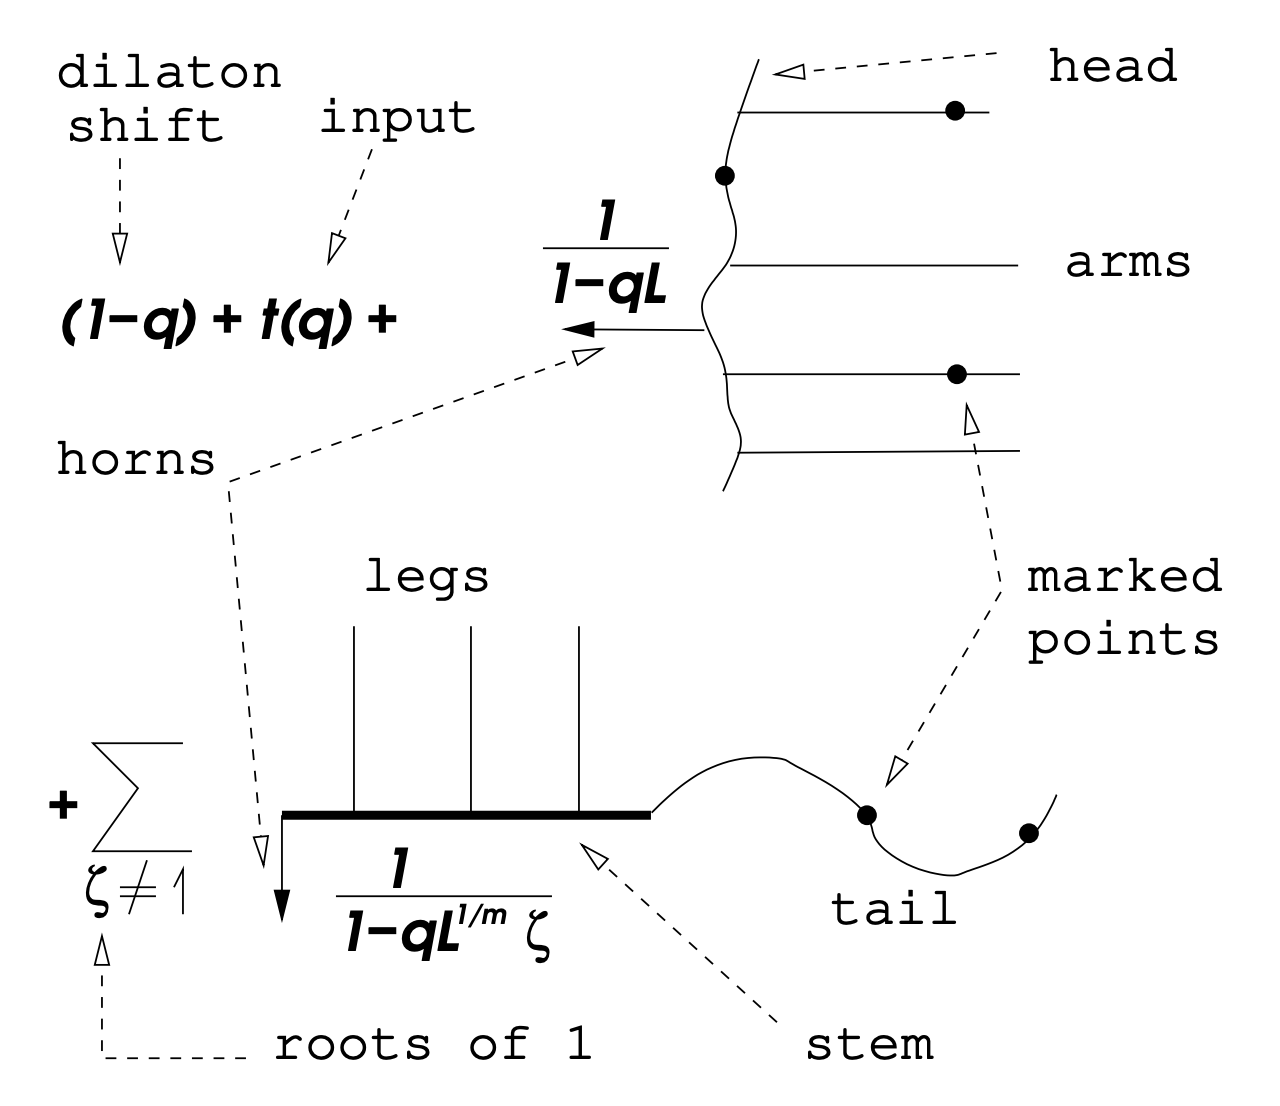
\includegraphics[width=0.8\textwidth]{givental.png}
    \caption{Givental-Tonita 给出的一种记录惯性分支的方式。}
    \label{fig:givental-png}
\end{figure}

\begin{figure}[htpb]
    \centering
    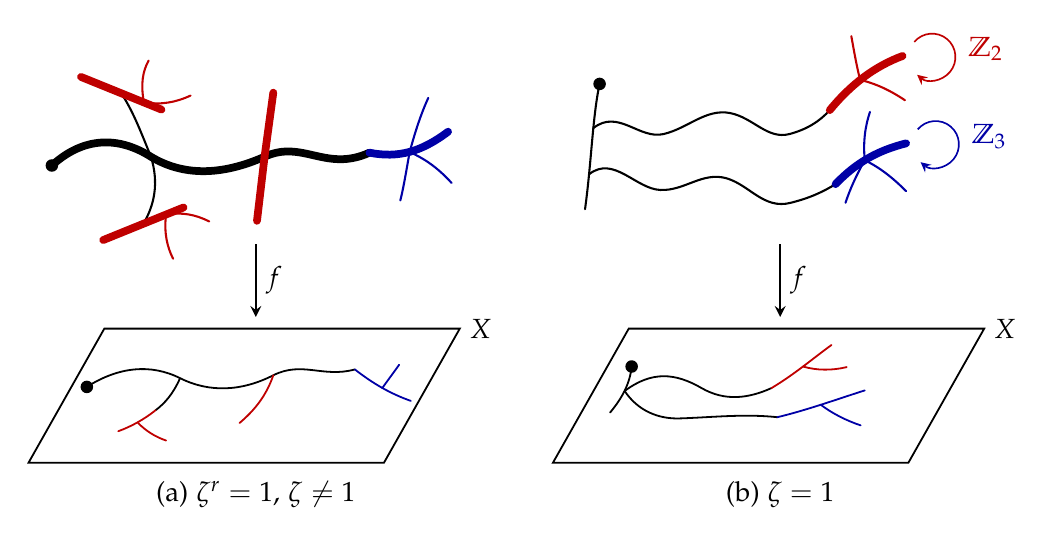
\begin{tikzpicture}[
        x=.74cm, y=.74cm,
        % Components of the domain curve. A cover style means the component
        % is a multiple cover of its image, drawn thick.
        dom/.style      ={black,         line width=.75pt, line cap=round},
        domcover/.style ={black,         line width=2.8pt, line cap=round},
        redcover/.style ={red!75!black,  line width=2.8pt, line cap=round},
        redtwig/.style  ={red!75!black,  line width=.75pt, line cap=round},
        bluecover/.style={blue!65!black, line width=2.8pt, line cap=round},
        bluetwig/.style ={blue!65!black, line width=.75pt, line cap=round},
        % Everything downstairs in X is drawn thin.
        img/.style      ={black,         line width=.65pt, line cap=round},
        redimg/.style   ={red!75!black,  line width=.65pt, line cap=round},
        blueimg/.style  ={blue!65!black, line width=.65pt, line cap=round},
        grparrow/.style ={->, >=stealth, line width=.6pt},
        fmap/.style     ={->, >=stealth, line width=.75pt},
        bull/.style     ={circle, fill=black, inner sep=1.6pt},
    ]

    %%%%%%%%%%%%%%%%%%%%%%%%%%%%%%%%%%%%%%%%%%%%%%%%%%%%%%%%%%%%%%%%%%%%%%%
    %% (a) zeta a primitive r-th root of unity, r >= 2.
    %%%%%%%%%%%%%%%%%%%%%%%%%%%%%%%%%%%%%%%%%%%%%%%%%%%%%%%%%%%%%%%%%%%%%%%
    \begin{scope}
        % The distinguished component: here g^r acts trivially on it, but g
        % does not, so it is a multiple cover of its image.
        \node[bull] at (-3.5,1.9) {};
        \draw[domcover]
            (-3.5,1.9)
            .. controls (-2.95,2.40) and (-2.35,2.40) .. (-1.80,2.05)
            .. controls (-1.25,1.72) and (-0.60,1.72) .. ( 0.15,2.05)
            .. controls ( 0.80,2.35) and ( 1.20,1.78) .. ( 1.95,2.12);

        % A leg meeting the distinguished component at a balanced node,
        % sticking out on both sides.  Each end carries a red multiple cover
        % together with the two branches interchanged by its automorphism.
        \draw[dom] (-1.80,2.05) .. controls (-2.00,2.55) and (-2.12,2.85) .. (-2.31,3.14);
        \draw[redcover] (-3.00,3.42) -- (-1.62,2.86);
        \draw[redtwig] (-1.92,2.98) .. controls (-1.98,3.30) and (-1.94,3.52) .. (-1.84,3.70);
        \draw[redtwig] (-1.92,2.98) .. controls (-1.62,2.94) and (-1.38,2.98) .. (-1.12,3.10);

        \draw[dom] (-1.80,2.05) .. controls (-1.66,1.60) and (-1.74,1.22) .. (-1.93,0.90);
        \draw[redcover] (-2.62,0.62) -- (-1.24,1.18);
        \draw[redtwig] (-1.54,1.06) .. controls (-1.58,0.74) and (-1.52,0.50) .. (-1.42,0.30);
        \draw[redtwig] (-1.54,1.06) .. controls (-1.26,1.10) and (-1.04,1.06) .. (-0.80,0.94);

        % A second balanced node, where the two legs are themselves the
        % multiple covers.
        \draw[redcover] (0.15,2.05) -- (0.30,3.15);
        \draw[redcover] (0.15,2.05) -- (0.02,0.95);

        % The tail: the part cut off at the unbalanced node.
        \draw[bluecover]
            (1.95,2.12) .. controls (2.45,2.02) and (2.85,2.14) .. (3.30,2.48);
        \draw[bluetwig] (2.64,2.13) .. controls (2.74,2.50) and (2.84,2.80) .. (2.96,3.06);
        \draw[bluetwig] (2.64,2.13) .. controls (2.58,1.80) and (2.54,1.54) .. (2.48,1.30);
        \draw[bluetwig] (2.64,2.13) .. controls (2.94,2.00) and (3.16,1.82) .. (3.36,1.60);

        \draw[fmap] (0,0.55) -- node[right] {$f$} (0,-0.70);

        % The target and the image of the map.
        \draw[img] (-3.9,-3.2) -- (2.2,-3.2) -- (3.5,-0.9) -- (-2.6,-0.9) -- cycle;
        \node[right] at (3.5,-0.9) {$X$};
        \node[bull] at (-2.90,-1.90) {};
        \draw[img] (-2.90,-1.90)
            .. controls (-2.35,-1.55) and (-1.80,-1.50) .. (-1.30,-1.75)
            .. controls (-0.80,-2.00) and (-0.25,-1.98) .. ( 0.30,-1.70)
            .. controls ( 0.80,-1.45) and ( 1.15,-1.75) .. ( 1.70,-1.60);
        % The two branches upstairs are folded onto the single one downstairs.
        \draw[img]    (-1.30,-1.75) .. controls (-1.42,-2.02) and (-1.56,-2.18) .. (-1.72,-2.30);
        \draw[redimg] (-1.72,-2.30) .. controls (-1.92,-2.46) and (-2.14,-2.58) .. (-2.36,-2.66);
        \draw[redimg] (-2.02,-2.52) .. controls (-1.88,-2.66) and (-1.72,-2.76) .. (-1.54,-2.82);
        \draw[redimg] ( 0.30,-1.70) .. controls ( 0.18,-2.05) and (-0.02,-2.30) .. (-0.28,-2.52);
        \draw[blueimg] (1.70,-1.60) .. controls (2.02,-1.85) and (2.32,-2.02) .. (2.66,-2.14);
        \draw[blueimg] (2.17,-1.92) .. controls (2.27,-1.78) and (2.36,-1.66) .. (2.46,-1.52);

        \node at (0,-3.75) {(a) \(\zeta^r = 1\), \(\zeta \neq 1\)};
    \end{scope}

    %%%%%%%%%%%%%%%%%%%%%%%%%%%%%%%%%%%%%%%%%%%%%%%%%%%%%%%%%%%%%%%%%%%%%%%
    %% (b) zeta = 1.
    %%%%%%%%%%%%%%%%%%%%%%%%%%%%%%%%%%%%%%%%%%%%%%%%%%%%%%%%%%%%%%%%%%%%%%%
    \begin{scope}[shift={(9,0)}]
        % Now g acts trivially on the distinguished component, so it is drawn
        % thin: it maps isomorphically onto its image.
        \node[bull] at (-3.10,3.30) {};
        \draw[dom] (-3.10,3.30) .. controls (-3.22,2.75) and (-3.24,1.95) .. (-3.35,1.15);
        \draw[dom] (-3.21,2.54)
            .. controls (-2.78,2.88) and (-2.42,2.34) .. (-2.00,2.44)
            .. controls (-1.58,2.54) and (-1.28,2.88) .. (-0.86,2.80)
            .. controls (-0.46,2.72) and (-0.22,2.34) .. ( 0.16,2.44)
            .. controls ( 0.46,2.52) and ( 0.68,2.66) .. ( 0.85,2.85);
        \draw[dom] (-3.28,1.75)
            .. controls (-2.86,2.08) and (-2.48,1.50) .. (-2.06,1.48)
            .. controls (-1.64,1.46) and (-1.34,1.80) .. (-0.92,1.68)
            .. controls (-0.52,1.56) and (-0.28,1.14) .. ( 0.18,1.26)
            .. controls ( 0.50,1.34) and ( 0.72,1.44) .. ( 0.95,1.58);

        % The arms: g acts nontrivially on them, through the indicated cyclic
        % group, which interchanges the thin branches sticking out.
        \draw[redcover] (0.85,2.85) .. controls (1.22,3.30) and (1.62,3.60) .. (2.10,3.78);
        \draw[redtwig] (1.37,3.37) .. controls (1.30,3.66) and (1.26,3.90) .. (1.22,4.12);
        \draw[redtwig] (1.37,3.37) .. controls (1.66,3.30) and (1.90,3.18) .. (2.14,3.02);
        \draw[grparrow, red!75!black]
            (2.30,4.02) arc[start angle=140, end angle=-130, radius=.40];
        \node[red!75!black, right] at (3.06,3.90) {$\Z_2$};

        \draw[bluecover] (0.95,1.58) .. controls (1.30,1.95) and (1.68,2.16) .. (2.16,2.28);
        \draw[bluetwig] (1.45,1.99) .. controls (1.42,2.32) and (1.46,2.58) .. (1.54,2.82);
        \draw[bluetwig] (1.45,1.99) .. controls (1.72,1.86) and (1.94,1.68) .. (2.16,1.46);
        \draw[bluetwig] (1.45,1.99) .. controls (1.30,1.72) and (1.20,1.50) .. (1.12,1.26);
        \draw[grparrow, blue!65!black]
            (2.36,2.52) arc[start angle=140, end angle=-130, radius=.40];
        \node[blue!65!black, right] at (3.12,2.40) {$\Z_3$};

        \draw[fmap] (0,0.55) -- node[right] {$f$} (0,-0.70);

        % The target and the image of the map.
        \draw[img] (-3.9,-3.2) -- (2.2,-3.2) -- (3.5,-0.9) -- (-2.6,-0.9) -- cycle;
        \node[right] at (3.5,-0.9) {$X$};
        \node[bull] at (-2.55,-1.55) {};
        \draw[img] (-2.55,-1.55) .. controls (-2.58,-1.85) and (-2.72,-2.10) .. (-2.92,-2.34);
        \draw[img] (-2.67,-1.97)
            .. controls (-2.20,-1.62) and (-1.80,-1.66) .. (-1.35,-1.92)
            .. controls (-0.95,-2.15) and (-0.55,-2.10) .. (-0.15,-1.92);
        \draw[img] (-2.67,-1.97)
            .. controls (-2.45,-2.30) and (-2.10,-2.46) .. (-1.70,-2.44)
            .. controls (-1.15,-2.42) and (-0.60,-2.36) .. (-0.05,-2.42);
        % Each arm is folded onto a single image curve with one branch.
        \draw[redimg] (-0.15,-1.92) .. controls (0.25,-1.68) and (0.55,-1.42) .. (0.88,-1.18);
        \draw[redimg] ( 0.39,-1.55) .. controls (0.63,-1.62) and (0.89,-1.62) .. (1.14,-1.56);
        \draw[blueimg] (-0.05,-2.42) .. controls (0.45,-2.30) and (0.95,-2.12) .. (1.45,-1.96);
        \draw[blueimg] ( 0.70,-2.21) .. controls (0.90,-2.36) and (1.14,-2.48) .. (1.38,-2.56);

        \node at (0,-3.75) {(b) \(\zeta = 1\)};
    \end{scope}
    \end{tikzpicture}
    \caption{\(I\bar{M}_{0,1}(X,\beta)\)的各个分支，由周祐正提供。}
    \label{fig:adelic-components}
\end{figure}

我们现在来解释~\Cref{fig:adelic-components}。设\(L_1\)为第一个标记点处的余切线，并设\(g\)为\(I\bar{M}_{0,1}(X,\beta)\)中一个点的自同构。则\(\zeta\)由条件“\(g\)在\(L_1\)上以特征值\(\zeta\)作用”定义。在两幅图中，实心点表示第一个标记点及其在\(X\)中的像，而粗的分支表示它是其像的多重覆盖。

首先，设\(\zeta = 1\)。则黑色分支是包含第一个标记点、且\(g\)在其上作为恒等作用的极大连通分支。红色与蓝色分支恰是\(g\)在其上非平凡作用的分支，我们称之为\textit{臂}。

现在设\(\zeta\)是某个\(r \geq 2\)的\(r\)次单位根。此时，黑色分支的结点必须关于\(g\)-作用是平衡的，所以我们切掉不平衡的部分，它被涂成蓝色，我们称之为\textit{尾}。在剩下的部分中，黑色分支是包含第一个标记点、且\(g^r\)在其上作为恒等作用的极大连通分支。最后，去掉黑色分支与尾之后，我们把剩余的分支称为\textit{腿}。

下面的定义归功于 Givental。我们写
\[ \ab<\frac{\Phi}{1-qL}>_{0,1,\beta}^{X,K} \coloneqq \sum_{\zeta} \ab<\frac{\Phi}{1-qL}>_{0,1,\beta}^{X_{\zeta}}, \]
其中\(X_{\zeta}\)项就是\(M_{\zeta}\)在 Riemann-Roch 定理下的贡献。现在，我们来定义臂、腿与尾。这里，我们定义\textit{臂}
\[ \mr{arm}(q) \coloneqq \sum_{\beta, \alpha, \zeta \neq 1} Q^{\beta} \Phi^{\alpha}\ab<\frac{\Phi_{\alpha}}{1-qL}>_{0,1,\beta}^{X_{\zeta}}, \]
\textit{腿}
\[ \mr{leg}_{\zeta}(q) \coloneqq \mr{leg}_r(q) = \Psi^r (\mr{arm}(q)), \]
以及\textit{尾}
\[ \mr{tail}_{\zeta}(q) \coloneqq \sum_{\beta, \alpha, \zeta' \neq \zeta} Q^{\beta} \Phi^{\alpha} \ab<\frac{\Phi_{\alpha}}{1-qL}>_{0,1,\beta}^{X_{\zeta'}}. \]

\begin{prop}[{\cite{GiventalTonita2014}}]
    J-函数在\(q = 1\)处的 Laurent 展开由
    \begin{align*}
        J^K(0)_{q=1} &= J^{\mr{fake}}(\mr{arm}(q)) \\
        &\coloneqq 1-q + \mr{arm}(q) + \sum_{n,\beta,\alpha} \frac{Q^{\beta}\Phi^{\alpha}}{n!} \ab<\frac{\Phi_{\alpha}}{1-qL}, \mr{arm}(L), \ldots, \mr{arm}(L)>_{0,n+1,\beta}^{\mr{fake}},
    \end{align*}
    给出，其中伪不变量通过应用 Riemann-Roch 并只考虑非扭曲扇区的贡献来计算。
\end{prop}

\begin{prop}[{\cite{GiventalTonita2014}}]
    在任何其他单位根\(\zeta \neq 1\)处，我们有
    \begin{align*}
        &J^K(0)_{q = \zeta} = (1-q) + \mr{tail}_{\zeta}(q) \\
        &+ \sum_{n,\beta,\alpha} \frac{Q^{r\beta}\Phi^{\alpha}}{n!} \ab[\frac{\Phi_{\alpha}}{1-\zeta q L^{1/r}}, \mr{leg}_r(L), \ldots, \mr{leg}_r(L), 1 - \zeta^{-1}L^{1/r} + \mr{tail}_{\zeta}(\zeta^{-1} L^{1/r})]^{\mr{stem}},
    \end{align*}
    其中茎是\(X \times B\mu_r\)的某个伪不变量，定义在模空间
    \[ \bar{M}_{0,n+2,\beta}^X(\zeta) \coloneqq \bar{M}_{0,n+2}(X \times B\mu_r, \beta, (g, 1, \ldots, 1, g^{-1})). \]
    上。它由公式
    \begin{align*}
        [\cdots]^{\mr{stem}} \coloneqq \int_{[\bar{M}_{0,n+2,\beta}^X(\zeta)]^{\vir}} \on{td}(T_{\bar{M}}) \on{ch}\ab(\frac{\on{Tr}(\cdots)}{\on{Tr}(\lambda_{-1}(N^*))}), 
    \end{align*}
    定义，其中\(N\)表示\(\bar{M}_{0,n+2,\beta}^X(\zeta) \subset \bar{M}_{0,nr+2}(X, r\beta)\)的法丛。
\end{prop}

\begin{rmk}
    若我们能计算伪理论与茎理论，则我们就能计算亏格零的量子 K 不变量。
\end{rmk}

\subsection{点的量子 K-理论}%
\label{sub:Quantum K-theory of a point}

一个自然的问题是研究高亏格量子 K-理论。我们从最简单的目标——一个点——开始。研究高亏格的一个动机是尝试证明 Calabi-Yau 四维流形上 GV 不变量的 Klemm-Pandharipande 定义、或 Calabi-Yau 五维流形上 GV 不变量的 Pandharipande-Zinger 定义的整性（在此情形下，我们只需考虑亏格\(1\)）。我们需要考虑点的量子 K-理论的一个原因是，在\(I\bar{M}_{1,1}(X, \beta)\)中，有一些分支上整条亏格\(1\)的曲线被收缩到一个点。

\begin{quest}
    K-理论的 Witten-Kontsevich 定理是什么？\footnote{据周祐正说，困难无处不在。}
\end{quest}

我们先回忆上同调的 Witten 猜想。我们从算子
\[ L = \partial_x^2 + u(x) \]
开始，并把它形变为
\[ \tilde{L} = \partial_x^2 + u(x, T_3, T_5, \ldots), \]
这里我们应把\(x = T_1\)，\(u(x) = u(x, 0, 0,\ldots)\)。形式地，利用对所有整数\(n \in \Z\)成立的性质
\[ \partial^n \circ f = \sum_{m = 0}^{\infty} \binom{n}{m} f^{(m)} \partial^{n-m} \]
写出
\[ L^{1/2} = \partial_x + \sum_{k > 0} a_{-k}(x) \partial_x^{-k} \]
。特别地，我们通过对所有\(k \geq 0\)的方程
\[ \pdv{\tilde{L}}{T_{2k+1}} = \ab[(\tilde{L}^{\frac{2k+1}{2}})_{\geq 0}, \tilde{L}] \]
构造 (2-)KdV 族。我们定义\textit{\(\tau\)-函数}为满足
\[ 2 \pdv[2]{}{x}\log \tau(x, T_3, T_5, \ldots) = u(x, T_3, T_5, \ldots). \]
的函数\(\tau\)。现在用\(u = 2x\)执行上述过程。定义函数
\[ F(t_0, t_1, \ldots) \coloneqq \sum_{n \geq 0} \sum_{k_0, \ldots, k_n} \ab<\tau_0^{k_0} \cdots \tau_n^{k_n}> \frac{t_0^{k_0} \cdots t_n^{k_n}}{k_0! \cdots k_n!}. \]
注意，由于亏格完全由插入项的个数与次数确定，记号
\[ \ab<\tau_0^{k_0} \cdots \tau_n^{k_n}> \]
唯一确定了点的一个后代 GW 不变量。

\begin{thm}[Kontsevich {\cite{Kontsevich1992}}]
    在变量替换\(t_i = (2i+1)!! T_{2i+1}\)下，\(F\)是从\(L = \partial_x^2 + 2x\)出发构造的 KdV 族的一个\(\tau\)-函数。
\end{thm}

该定理的一个应用是考虑虚局部化。例如，假设我们考虑\(\bar{M}_{g,0}(X, d[C])\)，其中\(C\)是 Calabi-Yau 三维流形中唯一的一条有理曲线，其法丛为\(N = \mc{O}(-1)\oplus \mc{O}(-1)\)。则在此情形下，我们可以归结到局部模型，并通过虚局部化计算
\begin{align*}
    \int_{[\bar{M}_{g,0}(\P^1, d)]^{\vir}} c_{\mr{top}}(R^1 \pi_* N) = \sum_{m \vdash d} \frac{(-1)^{d-L(m)}}{\abs{\Aut(m)}} \int_{\bar{M}_{g, L(m)}} \frac{1 + \cdots + c_g(\mc{H})}{\prod_i (1-m_i \psi_i)}
\end{align*}
。若我们想在 K-理论中得到类似的结果，则需要考虑形如
\[ \chi\ab(\bar{M}_{g, L(m)}/\Aut(m), \frac{\lambda_{-1}(\mc{H})}{1-m_i L_i}), \]
的项，因此我们需要考虑点的置换等变量子 K-理论。

我们现在做一个文献回顾。首先，李元斌~\cite{Lee1997}计算了公式
\[ \ab<\frac{1}{1-q_1 L}, \ldots, \frac{1}{1-q_n L}>_{0,n}^{\mr{pt}, K} = \ab(\prod_{i=1}^n \frac{1}{1-q_i}) \ab(1 + \sum_{i=1}^n \frac{q_i}{1-q_i})^{n-3}. \]
之后，李元斌–瞿枫~\cite{LeeQu2014}给出了一种原则上可以计算
\[ \ab<\frac{1}{1-q_1 L}, \ldots, \frac{1}{1-q_n L}>_{1,n}^{\mr{pt}, K} \]
的方法。Givental~\cite{Givental2017K1}计算了公式
\[ \sum_{n \geq 2} \ab<\frac{1}{1-q L}, 1, \ldots, 1>_{0,1+n}^{S_n} = (1-q) \exp\ab(\sum_{k > 0} \frac{\Psi^k}{k} \ab(1 + \frac{q}{1-q})). \]
最后，Milanov~\cite{Milanov2025}在一篇首次发布于 2024 年的预印本中计算了
\begin{align*}
    \sum_{n \geq 0}& \ab<\frac{1}{1-q_1 L}, \ldots, \frac{1}{1-q_r L}, 1, \ldots, 1>_{0,r+n}^{S_n} \\
    &= \ab(\prod_{i=1}^{r} \frac{1}{1-q_i})\ab(1 + \sum_{i=1}^r \frac{q_i}{1-q_i}) \exp\ab(\sum_{k > 0} \frac{\Psi^k}{k} \ab(1 + \sum_{i=1}^r \frac{q_i}{1-q_i})). 
\end{align*}

下面的多重 Hodge 递归以及基于它们的新的亏格一计算归功于周祐正，并在本次讲座中报告。

设\(s \in \Z\)，并定义多重 Hodge 层\(\mc{H}_s \coloneqq R^0 \pi_* (\omega_{\pi}^s)\)。考虑映射\(\bar{M}_{g,n+1} \xrightarrow{\pi} \bar{M}_{g,n}\)，我们把上方的余切线记为\(L_i\)，下方的记为\(\ell_i\)。

\begin{lem}
    对所有整数\(s\)与\(d_i\)，我们有
    \[ \pi_*\ab(\omega_{\pi}^s\ab(\sum_{i=1}^n d_i D_i)) = \mc{H}_s-\mc{H}_{1-s}^* + \sum_{i=1}^n \sum_{k=1}^{d_i} \ell_i^{-k+s}. \]
\end{lem}

\begin{rmk}
    注意，若\(f(q) \in \Z[q]\)，则\(\exp \sum_k \frac{\Psi^k}{k} (f(q)) \in \Z \ps{q}\)。原因是这个运算把\(f = \sum_{i=1}^{n} a_i q^i\)送到\(\prod_{i=1}^n \frac{1}{(1-q^i)^{a_i}}\)。
\end{rmk}

\begin{proof}
    当所有\(d_i\)为零时，由 Serre 对偶我们看到
    \[ R^0 \pi_* \omega_{\pi}^s - R^1 \pi_* \omega_{\pi}^s = \mc{H}_s - \mc{H}_{1-s}^* \]
    。下一步是证明
    \[ \pi_* \omega_{\pi}^s ((r+1)D_i) = \pi_* \omega_{\pi}^s(r D_i) + \ell_i^{s-r-1}. \]
    这里，我们先考虑正合列
    \[ 0 \to \mc{O} (-D_i) \to \mc{O} \to \mc{O}_{D_i} \to 0 \]
    并用\(\omega_{\pi}^s\)扭转，得到
    \[ 0 \to \omega_{\pi}^s(r D_i) \to \omega_{\pi}^s ((r+1)D_i) \to \omega_{\pi}^s ((r+1)D_i) \otimes \mc{O}_{D_i} \to 0 \]
    然后计算推前。
\end{proof}

\begin{lem}
    设\(f_i\)为有理函数，例如\(\frac{1}{1-q L}\)。则
    \begin{align*}
        \ab<f_1(L), \ldots, f_n(L), L_{n+1}^r>_{g, n+1} ={}& \sum_{i=1}^n \ab<f_1(L), \ldots, D(f_i f_{n+1}), \ldots, f_n(L)>_{g, n} \\
        &+ \ab<f_1(L), \ldots, f_n(L) \mid \mc{H}_r - \mc{H}_{1-r}^*>_{g,n},
    \end{align*}
    其中\(f_{n+1} = L_{n+1}^r\)，且\((Df)(x) \coloneqq \frac{f(x)-f(1)}{x-1}\)。
\end{lem}

为了证明它，我们需要考虑推前
\begin{align*}
    \pi_* (L_1^{d_1} \cdots L_{n+1}^{d_{n+1}}) &= \pi_* \ab(\pi^*(\ell_1^{d_1} \otimes \cdots \otimes \ell_n^{d_n}) \otimes \omega_{\pi}^{d_{n+1}}\ab(\sum_i (d_i+d_{n+1})D_i)).
\end{align*}
这里，我们用了\(L_i = (\pi^* \ell_i)(D_i)\)与\(L_{n+1} = \omega_{\pi}(D_1 + \cdots + D_n)\)这一事实。应用前一引理，我们看到推前变为
\[ (\ell_1^{d_1} \cdots \ell_n^{d_n})\ab(\mc{H}_{d_{n+1}} - \mc{H}_{1-d_{n+1}}^* + \sum_{i=1}^n \sum_{k=1}^{d_i + d_{n+1}} \ell_i^{-k+d_{n+1}}). \]
现在，李元斌的公式计算关联函数
\[ \ab<(L-1)^{k_1}, \ldots, (L-1)^{k_n}>_{0,n} = \frac{(n-3)!}{\prod_{i=1}^n k_i! \ab(n-3-\sum_i k_i)!} \]
，通过展开
\[ \frac{1}{1-qL} = \frac{1}{1-q} \sum_{k \geq 0} \frac{q^k(L-1)^k}{(1-q)^k}. \]
注意这里亏格\(0\)时没有 Hodge 丛，所以事实上该引理可以用来得到李元斌的公式。

\begin{lem}
    我们有
    \[ \mc{H}_r - \mc{H}_{1-r}^* = \pi^* (\mc{H}_r - \mc{H}_{1-r}^*) - \sum_{i=1}^n (D^2 (\pi^* \ell_i)^r) \mc{O}_{D_i}. \]
\end{lem}

这些引理合起来蕴含：我们可以归结到只有一个标记的情形，代价是插入项变得非常复杂，并且到处出现多重 Hodge 项。在亏格\(1\)时，事情变得容易一些，因为在\(\bar{M}_{1,1}\)上我们有
\[ \mc{H}_r = \mc{O}(r) = L_1^r. \]
在此情形下，回忆经典公式
\[ \chi\ab(\bar{M}_{1,1}, \frac{1}{1-qL}) = \frac{1}{(1-q^4)(1-q^6)}. \]
遗憾的是，计算
\[ \chi\ab(\bar{M}_{1,n}; \frac{1}{1-q_1 L} \cdots \frac{1}{1-q_n L}) \]
太难了，所以我们可以尝试计算
\[ \chi\ab(\bar{M}_{1,1}; \frac{1}{1-q_1 L_1} \cdots \frac{1}{1-q_n L_1})  \]
它是已知的，但如何为它写出一个好的公式并不清楚。我们考虑它的原因是运算
\[ \Z\ps{q} \xrightarrow{[]_r} \Z\ps{q_1, \ldots, q_r} \qquad q^k \to h_k(q_1, \ldots, q_r) \coloneqq \sum_{\ell_1 + \cdots + \ell_r = k} q_1^{\ell_1} \cdots q_r^{\ell_r}. \]
遗憾的是，周祐正不知道如何把
\[ \chi\ab(\bar{M}_{1,1}; \frac{1}{1-q_1 L_1} \cdots \frac{1}{1-q_n L_1}) = \ab[\frac{1}{(1-q^4)(1-q^6)}]_n \]
写成漂亮的形式。原则上我们可以写出像
\[ [f(q)]_2 \coloneqq \frac{q_1 f(q_1) - q_2 f(q_2)}{q_1 - q_2}, \]
这样的公式，但这似乎帮助不大。

\subsection{点的置换等变理论}%
\label{sub:Permutation-equivariant theory of a point}

我们可以用另一种方式计算\(\chi\ab(\bar{M}_{1,1}, \frac{1}{1-q L})\)。考虑椭圆曲线上的对合，它给出映射
\[ \bar{M}_{1,1} \to \bar{M}_{0,1+3}/S_3. \]
然后，Givental~\cite{Givental2017K1}计算出
\[ \chi\ab([\bar{M}_{0,1+n-1}/S_{n-1}], \frac{1}{1-qL}) = \prod_{i=2}^{n-1} \frac{1}{1-q^i}. \]
特别地，我们得到
\[ \frac{1}{(1-q^2)(1-q^3)}, \]
然后由于该映射是一个\(\mu_2\)-gerbe（或者说在对象层面是\(2:1\)覆盖），我们得到所要的公式。

考虑超椭圆轨迹\(\mc{H}_{g,1} \subset \bar{M}_{g,1}\)。注意标记位于一个 Weierstrass 点上。注意超椭圆对合的不动点映到\(\P^1\)上的\(2g+1\)个点，因此人们会想用计算
\[ \chi\ab(\bar{M}_{0,1+2g+1}/S_{2g+1}, \frac{1}{1-q L}) = \prod_{i=2}^{2g+1} \frac{1}{1-q^i} \]
来计算量
\(\chi\ab(\mc{H}_{g,1}, \frac{1}{1-qL})\)。然而，由于上方曲线退化的方式，我们需要考虑最后\(2g+1\)个标记的权为\(\frac{1}{2}\)的 Hassett 模空间~\cite{Hassett2003}。







\section{拟映射穿墙（周杨）}%
\label{sec:Quasimap wall-crossing (Yang Zhou)}

本讲座中的主要穿墙定理与主空间构造来自~\cite{Zhou2022}。更早的亏格零与高亏格结果见~\cite{CFK2014,CFK2020}，而稳定拟映射的基础见~\cite{CFKM2014}。

设\(X\)为五次三维流形。我们的目标是计数\(X\)上的亏格零曲线，这一问题已由 Givental 与连文豪–刘克峰–丘成桐解决。通过闭浸入\(X \subset \P^4\)，我们可以写出
\[ \bar{M}_0(X, d) \subset \bar{M}_0(\P^4, d), \]
后者是光滑的，并带有\((\C^{\times})^5\)的环面作用。若一个映射被此作用固定，则定义域必有一些分支映到不动点，另一些分支构成\(1\)维轨道的\(n :1\)覆盖。特别地，不动点轨迹由一组图所标记。

在此背景下，我们有量子 Lefschetz 原理，它断言
\[ [\bar{M}_0(X, d)]^{\on{vir}} = e(E) \cap [\bar{M}_0(\P^4, d)]. \]
这里向量丛\(E\)定义为
\[ E = \pi_* f^* \mc{O}(5), \]
其中\(\pi\)是泛曲线，\(f\)是泛稳定映射。我们将从另一个角度看待如下结果：若
\begin{align*}
    I(q, z) &= 1 + \sum_{d > 0} \frac{\prod_{k=1}^{5d} (5H+kz)}{\prod_{k=1}^d (H+kz)^5} q^d \in H^*(X)[z^{-1}] \ps{q} \\
    &= I_0(q) \cdot 1 + I_1(q) \frac{H}{z} + I_2(q) \frac{H^2}{z^2} + I_3(q) \frac{H^3}{z^3},
\end{align*}
则
\[ J (Q, z) = 1+ \sum_{d>0} \phi^{\alpha} \ab<\frac{\phi_{\alpha}}{z(z-\psi)}>_{0,1}^X Q^d = \frac{I}{I_0} \]
在相差镜映射\(Q = q \exp\ab(\frac{I_1}{I_0})\)的意义下成立。

\subsection{朴素计数}%
\label{sub:Naive counting}

我们考虑从固定的\(\P^1\)出发的“映射”\(\P^1 \to X \subset \P^4\)。为简单起见，我们假设\(X = \ab(\sum x_i^5 = 0)\)是 Fermat 五次超曲面。这样的映射由一组\([f_0, \ldots, f_4]\)给出，其中\(f_i \in \C[u,v]\)满足\(\deg f_i = d\)且\(\sum f_i^5 = 0\)。要成为真正的态射，我们需要\(f_i\)没有公共零点，但这个模不是紧合的，所以我们放宽此条件。于是我们考虑模空间
\[ QG(X, d) =  \ab\{ [f_0, \ldots, f_4] \middle\vert \Vectorstack{{ f_i \in \C[u,v] } { \deg f_i = d }}, \sum f_i^5 = 0, (f_0, \ldots, f_4) \neq (0,\ldots, 0) \} \bigg/ \C^{\times}. \]
它位于到射影空间的有理映射的相应模空间
\begin{align*}
    QG(\P^4, d) &\coloneqq  \ab\{ [f_0, \ldots, f_4] \mid f_i \in \C[u,v], \deg f_i = d, (f_0, \ldots, f_4) \neq (0, \ldots, 0) \} \\
    &\cong \P^{5d+5-1} 
\end{align*}
之中。这里有两个问题。第一，定义域是带参数化的，所以我们需要考虑\(\P^1\)的自同构。第二，为得到稳定映射，我们需要爆破定义域。

首先，令\(\C^{\times}\)通过缩放\(u\)作用于\(\P^1\)。考虑特殊的不动点轨迹\(F_{\star} \subset QG(X, d)\)，定义为
\[ F_{\star,d} = \ab\{ [f_0, \ldots, f_4] \text{被固定，且} (v=0) \text{不是公共零点} \}. \]
因此，\(F_{\star,d} = \ab\{ [a_0 u^d, \ldots, a_4 u^d] \mid [a_0, \ldots, a_4] \in X \} \cong X\)。从这一角度，利用形变理论中的标准论证，我们可以将 I-函数改写为
\begin{align*}
    I(q,z) &= \sum_{d > 0} \ab(\frac{[F_{\star, d}]^{\vir}}{e_{\C^{\times}}(N^{\vir})})^{\mr{PD}} q^d \\
    &= 1 + \sum_{d > 0} \ab( \frac{[X]}{e_{\C^{\times}}(N^{\vir})})^{\mr{PD}} q^d
\end{align*}
它位于\(H^*_{\C^{\times}}(X) \ps{q}[z^{-1}]\)中。

\subsection{不严格的穿墙}%
\label{sub:Wall-crossing without rigor}


其次，考虑带一个标记点外加一条尾的结点曲线\(C\)，其上有\(\C^{\times}\)的作用，并假设我们有映射\(f \colon C \to X\)。若取极限
\[ \lim_{t \to 0} [f_0(t^{-1}u, v), \ldots, f_4(t^{-1}u, v)] = [a_0 u^{d_0}, \ldots, a_4 u^{d_0}], \]
我们看到泡泡的极限落在\(F_{\star, d_0}\)中，其中公共零点远离结点。于是我们可以把这条尾替换为一个新的标记点，它携带 I-函数的某些项。对于五次超曲面，这就是\(I_1 H - I_0 \psi = [zI-z]_{+, z = -\psi}\)。这一过程结束时，我们只剩下\(C = \P^1\)以及 I-函数的各种贡献。

注意，若我们考虑\(\C^{\times}\)作用于\(\P^4\)，则\(f \colon C \to \P^4\)被固定当且仅当对所有\(t \in \C^{\times}\)，存在\(\varphi_t\)使得
\begin{equation*}
\begin{tikzcd}
    C \ar{r}{f} \ar{d}[swap]{\varphi_t} & \P^4 \\
    C \ar{ur}[swap]{t \cdot f}
\end{tikzcd}
\end{equation*}
交换。因此，我们得到\(\C^{\times}\)在定义域上的一个作用。

我们将定义到\(X\)的\(\ep\)-稳定拟映射的模空间\(Q_{g,n}^{\ep}(X, d)\)，它类似于稳定映射的模。我们希望把这些模空间看作彼此虚双有理的，并且每一个都是带完美障碍理论的紧合 DM 叠，因此我们可以定义拟映射不变量
\[ \ab< \gamma_1 \psi_1^{a_1} \cdots \gamma_n \psi_n^{a_n}>_{g,n}^{\ep} \coloneqq \int_{[Q_{g,n}^{\ep}(X,d)]^{\vir}} \prod_{i=1}^n \ev_i^*(\gamma_i) \psi_i^{a_i}. \]
这里\(\ep \in \Q_{>0}\)是一个正有理数。所有可能的\(\ep\)构成的空间具有墙与房室结构，其中墙出现在\(\frac{1}{n}\)处，\(n\)为正整数。当\(\ep > 1\)时我们得到 Gromov-Witten 理论（即稳定映射），而当我们向左移动时，允许的有理尾更少但基点更多。最终，在\(\ep \to 0^+\)极限下，不允许任何有理尾。最后，我们得到在\(\frac{1}{d_0}\)处的墙附近的如下穿墙公式：
\[ \ab<->_{g,n,d}^{\ep_+} - \ab<->_{g,n,d}^{\ep_-} = \sum_{k} \frac{1}{k!} \ab<-, \mu, \ldots, \mu>_{g,n+k, d-kd_0}^{\ep_+}. \]
这里\(\mu = [zI-z]_{+, q^{d_0}, z=-\psi}\)。在\(g = 0\)、\(n = 1\)、\(\ep = 0^+\)的特殊情形，我们得到
\[ \sum \phi^{\alpha} \ab<\frac{\phi_{\alpha}}{z(z-\psi)}>^{\ep}_{0,1} = I_{z^{<0}}. \]
从 GW 房室出发穿过所有的墙，我们得到
\[ I = 1 + \sum_{\substack{d \geq 1 \\ k \geq 0}} \frac{1}{k!} \sum_{\alpha} \phi^{\alpha} \ab< \frac{\phi_{\alpha}}{z(z-\psi)}, I_1 H - I_0 \psi, \ldots, I_1 H - I_0 \psi>_{0,1+k,d}^{\infty} q^d, \]
再由膨胀子方程与除子方程即可得出镜映射。

\subsection{拟映射}%
\label{sub:Quasimaps}

\begin{defn}
    到五次三维流形\(X\)的一个\textit{预稳定拟映射}由
    \[(C, x_1, \ldots, x_n, \mc{L}, \varphi_0, \ldots, \varphi_4),\]
    组成，其中\((C, x_1, \ldots, x_n)\)是预稳定曲线，\(\mc{L} \in \Pic C\)，且\(\varphi_0, \ldots, \varphi_4 \in H^0(C, \mc{L})\)，使得
    \[ \varphi^{-1}(0) \coloneqq \ab\{x \in C \mid \varphi_0(x) = \cdots = \varphi_4(x) = 0 \} \]
    是有限的且远离特殊点。此外，我们要求\(\sum \varphi_i^5 = 0\)。
\end{defn}

重要的是，我们将把\(\varphi^{-1}(0)\)称为\textit{基点}的集合。在\(\varphi^{-1}(0)\)之外，我们有一个真正的态射\(C \setminus \varphi^{-1}(0) \to X\)。从几何上看，假设我们有\(\A^1 \setminus 0\)上的一个族，在\(t \to 0\)的极限下零点轨迹\(\varphi_i^{-1}(0)\)最终会相撞。我们既可以在中心纤维中保留这个拟映射，也可以将中心纤维爆破若干次以得到真正的态射，其代价是泡出一条有理尾。因此，任何预稳定拟映射的模空间都不可能是分离的，所以我们必须考虑某种稳定性条件。

\begin{defn}
    预稳定拟映射\((C, \mathbf{x}, \mc{L}, \varphi)\)称为\textit{\(\ep\)-稳定}的，若
    \begin{enumerate}
        \item 对所有\(x \in \varphi^{-1}(0)\)，有\(\on{len}(x) \leq \frac{1}{\ep}\)，其中\(\on{len}(x) = \min \ab\{ \on{ord}_x (\varphi_i)\}\)；
        \item \(\Q\)-线丛\(\mc{L}^{\ep} \otimes \omega_C^{\log}\)在\(C\)的每个不可约分支上都有正的次数。
    \end{enumerate}
\end{defn}

注意，对所有不可约分支\(C' \subseteq C\)，我们有\(\deg \mc{L}|_{\mc{C}'} \geq 0\)。因此，会发生变化的只有带\(\leq 2\)个特殊点的亏格\(0\)曲线或没有标记点的亏格\(1\)曲线。注意在\((0,0)\)与\((1,0)\)情形，我们有\(C = C'\)，而在\((0,2)\)情形，稳定性等价于\(\deg \mc{L} > 0\)，故在\((0,1)\)情形，第二个条件等价于
\[ \deg \mc{L}|_{C'} > \frac{1}{\ep}. \]

\begin{exm}
    在\(\ep > 1\)房室中，注意第一个条件蕴含没有基点，第二个条件蕴含所有不稳定分支都有正的次数，因此我们恢复了稳定映射。

    若我们移动到\(\frac{1}{2} < \ep < 1\)的房室，则必须收缩次数为\(1\)的有理尾。例如，若我们有一条由两条次数\(1\)的有理曲线组成、末端为一条尾的链，那么我们收缩最外侧的尾，剩下一条次数\(2\)的有理尾，其上带一个长度为\(1\)的基点。

    若我们移动到\(\frac{1}{3} < \ep < \frac{1}{2}\)的房室，则必须收缩所有次数为\(2\)的有理尾，并将它们替换为长度为\(2\)的基点。
\end{exm}

\begin{rmk}
    在射影空间的情形，存在一个真正的态射
    \[ Q_g^{\ep_+}(\P^N, d) \to Q_g^{\ep_-}(\P^N, d) \qquad (C_g \cup C_0, \mc{L}, \varphi) \mapsto (C_g, \mc{L}|_{C_g}(p), \varphi(p)). \]
    对于一般的靶空间，这是不可能的，但这一想法为拟映射穿墙现象提供了直观。
\end{rmk}

我们现在讨论如何将此推广到更一般的靶空间。设
\[ X = V \sslash_{\theta} G, \]
其中\(V\)是仿射的，\(G\)是约化的，\(\theta\)是\(G\)的一个特征标。我们需要要求
\begin{enumerate}
    \item \(V^{\mr{ss}}(\theta) = V^s(\theta) \neq \emptyset\)；
    \item \(V\)至多有 lci 奇点，且\(V^s(\theta)\)是光滑的。
\end{enumerate}
注意我们要求稳定轨迹具有有限稳定子。为方便起见，我们还要求
\begin{enumerate}
    \item \(V \sslash G\)是射影的；
    \item \(G\)在稳定轨迹上自由作用。
\end{enumerate}

\begin{exm}
    在五次超曲面的情形，\(V\)是五次超曲面上的仿射锥。不稳定轨迹由原点组成，它是唯一的奇点。
\end{exm}

\begin{exm}
    另一个例子是，我们可以考虑带一般稳定性条件的\(\C^N \sslash (\C^{\times})^r\)，得到一个环面簇。
\end{exm}

\begin{exm}
    我们可以考虑 Grassmann 簇
    \[ G(2,4) = M_{2\times 4} \sslash GL_2, \]
    其中不稳定轨迹由秩严格小于\(2\)的矩阵组成。
\end{exm}

\begin{rmk}
    当\(G\)是交换群时，对于一般的稳定性条件，关于稳定轨迹的条件总是满足的；但对非交换的\(G\)，这并不总是可能的。
\end{rmk}

\begin{rmk}
    对于一般的光滑射影簇，原点未必是 lci 的，所以尚不清楚如何以仍能定义虚闭链的方式定义拟映射。
\end{rmk}

\begin{defn}
    到\(V \sslash G\)的一个\textit{预稳定拟映射}是一个映射\(u \colon C \to [V/G]\)，使得基轨迹
    \[ u^{-1}([V^{\mr{un}}(\theta) / G]) \]
    是有限的且远离特殊点。按定义，\(u\)由一个主\(G\)-丛\(P \to C\)连同一个等变映射\(P \to V\)组成，这等价于相伴丛\(P \times_G V\)的一个截面。
\end{defn}

\begin{exm}
    对于五次超曲面，这恰好恢复了一个线丛\(\mc{L} \in \Pic C\)（它等价于一个\(\C^{\times}\)-挠子）连同\(\on{Tot}(\mc{L}^{\oplus 5})\)的一个满足定义方程的截面。
\end{exm}

为了定义次数，我们可以考虑\([V/G]\)上的线丛\(\mc{L}_{\theta}\)。然后我们可以把\(C' \subset C\)在\(u\)下的次数定义为
\[ \deg (u^* \mc{L}_{\theta}|_{C'}). \]

\begin{exm}
    在\(G(2,4)\)的例子中，注意一个主\(\on{GL}_2\)-丛等价于\(C\)上的一个秩\(2\)向量丛\(\mc{E}\)。因此，\(P \times_G V\)等价于\(\mc{E}^{\oplus 4}\)这一数据，从而到 Grassmann 簇的拟映射等价于稳定商。在此情形，我们寻找的是一般满的
    \[ \mc{O}^{\oplus 4} \to \mc{E}, \]
    并且由于\(\theta = \det\)，我们看到\(u^* \mc{L}_{\theta} = \det \mc{E}\)。
\end{exm}

\begin{exm}
    考虑\(V = \C^{N+1}\)，并注意\(\P^N = V \sslash \C^{\times}\)。若我们考虑\(\theta_1 \colon z \mapsto z\)，则有
    \[ V^{\on{un}} = V((x_i)). \]
    然而，若我们考虑\(\theta \colon z \mapsto z^2\)，则有
    \[ V^{\on{un}} = V((x_i x_j)). \]
\end{exm}

这里我们看到概形结构依赖于特征标的选取，所以我们不能简单地朴素定义基点的长度。注意
\[ V^{\on{un}} = V\ab(\ab< \bigoplus_{k \geq 1} R_k>), \qquad R_k = H^0([V/G], L_{\theta}^{\otimes k}). \]
特别地，我们必须定义
\[ \on{len}(x) \coloneqq \min_{\substack{f \in R_k \\ k \geq 1}} \frac{\on{ord}_x u^*(f)}{k}. \]

\begin{exm}
    设\(X = \mr{pt} = \C \sslash_{\theta} \C^{\times}\)。则一个预稳定拟映射就是
    \[ (C, \mc{L}, \varphi \in H^0(\mc{L})), \]
    其中\(\varphi^{-1}(0)\)是有限的且远离特殊点。此外，若\(\deg \mc{L} = 1\)，我们恰好恢复了\(C^{\mr{sm}}\)中一个新标记点的数据。
\end{exm}

\begin{exm}
    现在考虑\(X = \mr{pt} = \C^n \sslash (\C^{\times})^n\)。并假设次数为\((1, \ldots, 1)\)。现在我们令
    \[ \theta = (a_1, \ldots, a_n). \]
    因此，注意
    \[ \ab<R_1> = \ab<(x_1^{a_1} \cdots x_n^{a_n})>. \]
    由于这些都位于次数\(1\)，我们看到对光滑点\(x \in C^{\mr{sm}}\)，有
    \[ \on{len}_x = \sum \on{ord}_x (\varphi_i^{a_i}) = \sum a_i \on{ord}_x \varphi_i. \]
    若我们令\(\ab\{p_i\} = \varphi_i^{-1}(0)\)，则条件\(\ep \cdot \on{len}(x) \leq 1\)等价于要求
    \[ \sum_{x = p_i} \ep a_i \leq 1. \]
    此时次数条件成为
    \[ \ep \sum_i a_i + \deg \omega_C > 0. \]
    等价地，这是说
    \[ \omega_C(\ep a_1 p_1 + \cdots + \ep a_n p_n) > 0, \]
    所以我们恢复了权为\((\ep a_1, \ldots, \ep a_n)\)的带权带点曲线。
\end{exm}

\subsection{主空间}%
\label{sub:Master space}

证明用到虚局部化~\cite{GP1999}；Hassett 的带权模空间~\cite{Hassett2003}为该构造提供了一个模型。

我们的方法是在一个插值于两个模之间的主空间上进行虚局部化。考虑\(\P^n\)上由下式给出的\(\C^{\times}\)-作用
\[ t \cdot [x_0 : \cdots : x_n] = [t x_0, x_1, \ldots, x_n]. \]
不动点轨迹由\(x_0 = 0\)处的一个\(\P^{n-1}\)和一个点\([1, 0, \ldots, 0]\)组成。于是我们可以计算
\[ \int_{\P^{n-1}} H^{n-1} = 1 \]
方法是把计算转移到另一个不动点轨迹上。特别地，我们提升到\(H \in H_{\C^{\times}}^* (\P^n) = \Q[H,z] / (H-z)H^n\)并计算
\begin{align*}
    \int_{\P^n} H^{n-1} &= \int_{\P^{n-1}} \frac{H^{n-1}}{-z+H} + \int_{\mr{pt}} \frac{z^{n-1}}{z^n}.
\end{align*}
取留数，我们看到
\begin{align*}
    0 &= \on{Res}_{z = 0}\int_{\P^{n-1}} \frac{H^{n-1}}{-z+H} + 1 \\
    &= 1 - \int_{\P^{n-1}}H^{n-1},
\end{align*}
这就恢复了所需的积分。我们在这里用到的关键事实是射影空间是紧合的。

\begin{exm}[第二个玩具例子]
    我们考虑第二个玩具例子。回忆 Hassett 的带权带点曲线的模
    \[ (C, x_1, \ldots, x_n) \]
    其中\(C\)是结点曲线，且\(x_i \in C^{\mr{sm}}\)可以相撞。相撞由如下方式调控：每个标记点被赋予一个权\(\delta_i \in \Q \cap (0,1]\)，并要求满足下列条件：
    \begin{enumerate}
        \item 对所有\(x \in C^{\mr{sm}}\)，有
            \[ \sum_{x = x_i} \delta_i \leq 1; \]
        \item 我们有稳定性条件\(\omega_C(\delta_1 x_1 + \cdots + \delta_n x_n) > 0\)。例如，若我们有一条有理尾，则\(\sum_{x_i \in C'} \delta_i > 1\)。
    \end{enumerate}
\end{exm}

\begin{exm}[另一个玩具例子]
    我们的目标是再一次计算
    \[ \int_{\bar{M}_{0,4}} \psi_1 = 1. \]
    我们的第一个目标是改变稳定性条件。若我们令
    \[ \delta_+ = \ab(\frac{2}{3}, \frac{2}{3}, \frac{2}{3}, \frac{2}{3}), \]
    我们看到稳定性条件没有改变。然而，若我们令
    \[ \delta_- = \ab(\frac{2}{3}, \frac{2}{3}, \frac{2}{3}, \frac{1}{3}), \]
    模空间没有改变，但泛曲线实际上变成了\(\P^1 \times \P^1\)，其中截面\(x_4\)是对角线。这告诉我们
    \[ \int_{\bar{M}_{0,4}^{\delta_-}} \psi_1 = 0, \]
    我们将利用这一点在\(\delta_+\)房室中进行计算。我们可以尝试通过既允许带\(x_i, x_4\)的有理尾又允许\(x_1 = x_4\)来构造主空间，但如果这样做，我们会得到一个带有理尾且\(x_1 = x_4\)的半稳定点。我们希望通过从主空间取商来得到它，所以我们在模中加入一个切向量的数据。因此，定义\(\delta_{\pm}\)主空间由形如
    \[ \xi = (C, x_1, \ldots, x_4, v \in T_{x_4} C \cup \infty) \]
    的对象组成，其中\(C\)是结点曲线，\(x_i\)是光滑点，\(x_1, x_2, x_3\)互不相交，
    \[ \sum_{x_i \in C'} \frac{2}{3} \delta_i > 1 \]
    对所有有理尾\(C'\)成立，若\(v = 0\)，则\(x_4\)与其他\(x_i\)不相交，而当\(v = \infty\)时，不存在使得\(x_4 \neq x_i\)（\(i = 1,2,3\)）的有理尾。

    我们现在通过缩放\(v\)赋予这个主空间一个\(\C^{\times}\)的作用。有若干不动点轨迹：
    \begin{enumerate}
        \item 当\(v = 0\)时，我们得到\(\bar{M}_{0,4}^{\delta_+}\)；
        \item 当\(v = \infty\)时，我们得到\(\bar{M}_{0,4}^{\delta_-}\)；
        \item 还有\(v \neq 0,\infty\)且我们有一条满足\(x_i = x_4\)的有理尾的不动点轨迹。
    \end{enumerate}

    若我们考虑一个一般点（四个标记点互不相交），它沿\(\C^{\times}\)-作用将直接回到自身。然而，若我们从一条包含\(x_1\)与\(x_4\)的有理尾出发，则我们首先到达一条\(v\)一般但\(x_1 = x_4\)的有理尾，而若我们光滑化结点，则得到一条\(x_1 = x_4\)的单个曲线，但我们允许\(v \to \infty\)，这是另一个不动点。现在我们可以积分
    \begin{align*}
        \int_{\ms{Master}} \psi_1 = \int_{\bar{M}_{0,4}^{\delta_+}} \frac{\psi_1}{-z-?} + \int_{\bar{M}_{0,4}^{\delta_-}} \frac{\psi_1}{z+?} + \on{Cont}(12|34) + \on{Cont}(13|24) + \on{Cont}(14|23).
    \end{align*}
    在\(z = 0\)处取留数，我们得到
    \begin{align*}
        0 &= - \int_{\bar{M}_{0,4}^{\delta_+}} \psi_1 + 0 + 0 + 0 + \int_{\mr{pt}} \frac{(-z)}{(\pm z)(\pm z)},
    \end{align*}
    其中最后一项分母中的\(\pm z\)是结点光滑化参数，因此我们恢复了所需的积分。
\end{exm}

有了所有这些玩具例子，我们终于可以讨论拟映射主空间了。在\(\frac{1}{d_0}\)墙处，我们的第一步是同时允许次数\(d_0\)的有理尾和长度\(d_0\)的基点。然而，我们可以考虑带一条有理尾且拟映射形如
\[ [a_0 u^{d_0}, \ldots, a_n u^{d_0}], \]
的曲线，它们有无穷多个自同构。然而，我们不能在基点处附加切向量（因为形变会移除它们），而且还存在这样的情形：存在多于一条次数\(d_0\)的尾带有长度\(d_0\)的基点（此时自同构群包含\(\C^{\times}\)）。

\begin{rmk}
    有一个关键的观察。假设我们有两条次数\(d_0\)的有理尾，并把两个结点记为\(p_1\)和\(p_2\)。现在定义光滑化参数的空间
    \[ \C \cong \Theta_i = T_{p_i} E_i \otimes T_{p_i} C_g, \]
    其中\(E_i\)是有理尾，\(C_g\)是曲线的其余部分。我们将考虑以次数标记的带权半稳定曲线的模
    \[ \mf{M}_{g,n,d}^{\mr{wt}} \xrightarrow{\text{\'et}} \mf{M}_{g,n} \]
    注意这个态射是高度不分离的。我们将考虑开子叠\(\mf{M}_{g,n,d}^{\mr{wt}, \ep_0}\)，其中曲线没有次数严格小于\(d_0\)的尾。然后我们可以考虑 Cartier 除子\(\mc{Z}\)，其上存在至少一条次数\(d_0\)的尾。特别地，我们看到
    \[ \Theta_i = N_{\mc{Z}_i} |_{\xi} \]
    对所关心的点处的两个分支\(\mc{Z}_1\)和\(\mc{Z}_2\)成立。我们还看到\(\Theta_1 \otimes \Theta_2\ = \mc{O}(\mc{Z})|_{\xi}\)，所以我们可以加入数据
    \[ v \in \ab(\bigotimes_i \Theta_i)^{\vee} \cup \ab\{\infty\} \]
    以及数据
    \[ w \in \P(\Theta_1 \oplus\Theta_2). \]
\end{rmk}

实际的构造如下进行。考虑\(\mc{Z} \subset \mf{M} = \mf{M}_{g,d}^{\mr{wt}, \ep_0}\)。定义\(\tilde{\mf{M}} \to \cdots \to \mf{M}\)为沿\(\mc{Z}\)的各层的迭代爆破。那么主空间在概形\(S\)上的一个对象（带校准尾的拟映射）由如下数据给出：一个拟映射
\begin{equation*}
\begin{tikzcd}
    C \ar{d} \ar[dashrightarrow]{r}{f} & X \\
    S
\end{tikzcd}
\end{equation*}
它诱导态射\(p \colon S \to \mf{M}_{g,d}^{\mr{wt}, \ep_0}\)；一个提升的选取
\begin{equation*}
\begin{tikzcd}
    & \tilde{\mf{M}} \ar{d}{\tau} \\
    S \ar{r}{p} \ar[dashrightarrow]{ur}{w} & \mf{M}_{g,d}^{\mr{wt}, \ep_0},
\end{tikzcd}
\end{equation*}
一个线丛\(\mc{N} \in \Pic S\)，以及\(v = (v_1, v_2)\)，其中\(v_1 \in H^0(w^* \mc{O}(-\mc{Z}))\)，\(v_2 \in H^0(\mc{N})\)，且\((v_1, v_2)\)处处不为零。我们还不允许长度严格大于\(d_0\)的基点，并要求如下稳定性：
\begin{enumerate}
    \item 当\(v = 0\)时，我们得到\(\ep_+\)-稳定性；
    \item 当\(v = \infty\)时，我们得到\(\ep_-\)-稳定性；
    \item 任何常值尾（次数\(d_0\)且带长度\(d_0\)的基点）都是纠缠尾。这里，我们考虑使得\(w\)映到例外轨迹\(\bigcap_{i \in I} \tilde{\mc{Z}}_i\)的最后一次爆破，此时对\(i \in I\)，\(E_i\)是纠缠尾；
    \item 若存在一条次数\(d_0\)的尾，则所有长度\(d_0\)的基点都位于次数\(d_0\)的尾上。
\end{enumerate}






\section{对数 GLSM（陈琪乐）}%
\label{sec:Log GLSM (Qile Chen)}

设 \(X\) 是一个光滑射影簇（甚至可以是 DM 叠）。设 \(E\) 是 \(X\) 上的一个向量丛，带有截面 \(s \in H^0(E)\)，其零点轨迹 \(Z\) 光滑且具有预期余维数。我们称 \(X\) 与 \(E\) 为环境空间，称 \(s\) 与 \(Z\) 为完全交。

\begin{quest}
    \(Z\) 的 GW 理论与 \((X, E)\) 的 GW 理论之间有什么关系？
\end{quest}

当 \(g = 0\) 时，Givental 以及连文豪–刘克峰–丘成桐利用这一关系计算了完全交的 GW 不变量；当 \(g = 1\) 时，这由 Zinger 完成。一般而言有两种途径：(N)MSP 与对数 GLSM。在本系列讲座中，我们将讨论对数 GLSM。\footnote{陈琪乐建议听众若对 MSP 有疑问，可以去请教本笔记作者与周杨。}

\subsection{R-映射}%
\label{sub:R-maps}

我们考虑 \textit{R-环面} \(\C^{\times}_{\omega} \coloneqq \C^{\times}\)。它有一个权为 \(1\) 的表示，记作 \(\C_{\omega}\)。它下降为 \(B \C_{\omega}^{\times}\) 上的一个线丛 \(\mc{L}_{\omega} \coloneqq [\C_{\omega} / \C^{\times}_{\omega}]\)。R-映射的靶空间是叠
\[ \P \to B \C^{\times}_{\omega} \]
它们是 DM-型、分离且（对数）光滑的。现在，一个 R-映射由如下（2-）交换图组成：
\begin{equation*}
\begin{tikzcd}
    & \mf{P} \ar{d} \\
    C \ar{ur}{f} \ar{r}[swap]{\omega^{\log}} \ar{d} & B \C_{\omega}^{\times} \\
    S.
\end{tikzcd}
\end{equation*}
这里的曲线可以是预稳定的、扭曲的、对数的，甚至是穿孔的。

\begin{exm}
    我们的第一个例子是稳定映射。令 \(\mf{P} = B\C_{\omega}^{\times}\)。由于在图
    \begin{equation*}
    \begin{tikzcd}
        & X \times B\C_{\omega}^{\times} \ar{d} \\
        C \ar{ur} \ar{r} & B \C_{\omega}^{\times}
    \end{tikzcd}
    \end{equation*}
    中竖直箭头是第二投影，我们看到这归结为到 \(X\) 的一个映射。
\end{exm}

\begin{exm}
    考虑映射
    \begin{equation*}
    \begin{tikzcd}
        & \mc{L}_{\omega} \ar{d} \\
        C \ar{ur}{f} \ar{r} & B \C_{\omega}^{\times}.
    \end{tikzcd}
    \end{equation*}
    若假设 \(C\) 无标记点，我们看到这个映射的数据就是 \(\omega_C\) 的一个截面，因此我们重新得到了全纯微分。
\end{exm}

\begin{exm}
    考虑由 \(z \mapsto z^{r_{\mr{in}}}\) 给出的态射 \(\C^{\times}_R \to \C^{\times}_{\omega}\)。于是我们看到
    \[ \mc{L}_R^{\otimes r_{\mr{in}}} \simeq \mc{L}_{\omega} |_{B \C_R^{\times}}. \]
    现在，一个图
    \begin{equation*}
    \begin{tikzcd}
        & B \C_R^{\times} \ar{d} \\
        C \ar{ur}{f} \ar{r} & B \C_{\omega}^{\times}
    \end{tikzcd}
    \end{equation*}
    （其中 \(C\) 无标记点）等价于一个线丛 \(\mc{L}_R|_C\) 连同一个同构 \(\mc{L}_R^{\otimes r_{\mr{in}}} \simeq \omega_C\) 的数据。另外，我们也可以考虑如下形式的 R-映射
    \begin{equation*}
    \begin{tikzcd}
        & \mc{L}_R \ar{d} \\
        & B \C_R^{\times} \ar{d} \\
        C \ar{uur}{f} \ar{r} & B \C_{\omega}^{\times},
    \end{tikzcd}
    \end{equation*}
    它们参数化带有 R-旋量线丛及其一个截面的曲线。
\end{exm}

\begin{exm}
    设 \(X\) 是光滑射影簇。考虑如下形式的 R-映射
    \begin{equation*}
    \begin{tikzcd}
        & E^{\vee} \boxtimes \mc{L}_{\omega} \ar{d} \\
        & X \times B \C_{\omega}^{\times} \ar{d} \\
        C \ar{uur}{f} \ar{r} & B \C_{\omega}^{\times}.
    \end{tikzcd}
    \end{equation*}
    这等价于一个映射 \(C \to X\) 连同一个截面 \(\rho \in H^0(E^{\vee}|_C \otimes \omega_C)\)。
\end{exm}

我们来考虑 GW 情形下的靶空间。
考虑环境空间的数据 \((X, E)\)。我们令 \(\mf{P}^{\circ} \coloneqq E^{\vee} \boxtimes \mc{L}_{\omega}\)。态射 \(\mf{P}^{\circ} \to B \C_{\omega}^{\times}\) 非常好，但它不是紧合的。为了弥补这一点，我们考虑对数叠
\[ \mf{P} = ( \P(E^{\vee} \boxtimes \mc{L}_{\omega} \oplus \mc{O}) , \infty). \]
由于这是光滑叠中的一个光滑除子，映射 \(\mf{P} \to B \C_{\omega}^{\times}\) 是紧合且对数光滑的。注意我们有零截面
\[ 0_{\mf{P}} \subset \mf{P}^{\circ} \subset \mf{P} \supset \infty. \]

现在考虑 r-旋量情形下的靶空间。考虑对数叠
\[ (\P(\mc{L}_R^{\oplus n} \oplus \mc{O}), \infty) = \mf{P} \to B \C_R^{\times} \to B \C_{\omega}^{\times}. \]
这个态射是紧合且对数光滑的。

\subsection{对数与穿孔 R-映射}%
\label{sub:Log and punctured R-maps}

我们考虑图
\begin{equation*}
\begin{tikzcd}
    & \mf{P} \ar{d} \\
    C \ar{ur}{f} \ar{r}[swap]{\omega^{\log}} \ar{d} & B \C_{\omega}^{\times} \\
    S
\end{tikzcd}
\end{equation*}
其中 \(C \to S\) 是一条对数曲线或穿孔（可能扭曲的）曲线，而 \(S\) 是一个 fs 对数概形。GW 情形下的稳定性条件是：\(f\) 可表，并且
\[ (\omega_{\log})^{1+\delta} + H^{\otimes k} \otimes f^* \mc{O}(\infty) > 0 \]
对所有 \(0 < \delta \ll 1\) 与 \(k \gg 1\) 成立，其中 \(H\) 是 \(X\) 的粗模空间上的一个丰富线丛。对于穿孔 R-映射，我们还要求预稳定性。

\begin{exm}
    考虑全纯微分的情形。考虑 \(f \in H^0(\omega_C)\)，使得其所有零点都集中在一个 Weierstrass 点上，其中 \(C\) 的亏格为 \(2\)。若考虑 \(\lim_{\lambda \to \infty} \lambda \cdot f\)，则极限由一个整体映到 \(\infty\) 的亏格 \(2\) 分支和一个记住了该零点的有理分支组成。
\end{exm}

我们现在讨论对数或穿孔 R-映射的热带化。回忆一个图
\[ \ul{G} = (\V, \H, \imath \colon \H \to \H, v \colon \H \to \V) \]
由顶点集 \(\V\)、半边集 \(\H\)、半边上的一个对合 \(\imath\)，以及从半边到顶点的根映射组成。我们令腿的集合 \(\L\) 为
\[ \L = \ab\{ h \in \H \mid \imath(h) = h\}. \]
边是在对合下互相对应的一对不同半边：
\[ \E = \ab\{ \ab\{h, \hat{h}\} \mid \imath(h) = \hat{h} \neq h \}. \]
现在，一个装饰图是一个图连同一个亏格函数
\[ g \colon \V \to \N, \]
一个指派
\[ r \colon \H \to \N, \]
以及一个排序
\[ m \colon \L \to \ab\{0, \ldots, n\}. \]

\begin{exm}
    \leavevmode\par
    \begin{center}
    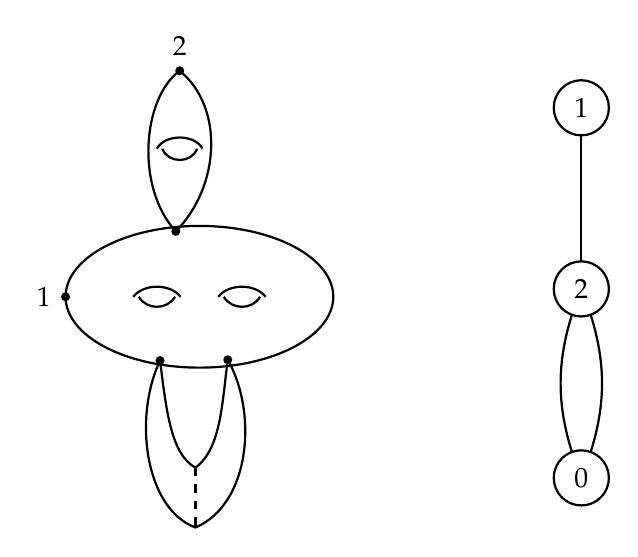
\begin{tikzpicture}[
        x=1cm,
        y=1cm,
        curve component/.style={thick},
        marked point/.style={circle,fill=black,inner sep=1.15pt},
        graph vertex/.style={
            circle,draw,thick,fill=white,minimum size=7mm,inner sep=0pt
        }
    ]
        % A three-component curve with components of genera 1, 2, and 0.
        \draw[curve component] (1.5,3.65) ellipse [x radius=1.7,y radius=0.9];

        % The two handles on the genus-two component.
        \draw[curve component]
            (0.66,3.65)
            .. controls (0.79,3.82) and (1.13,3.82) .. (1.26,3.65);
        \draw[curve component]
            (0.73,3.65)
            .. controls (0.83,3.48) and (1.09,3.48) .. (1.19,3.65);
        \draw[curve component]
            (1.74,3.65)
            .. controls (1.87,3.82) and (2.21,3.82) .. (2.34,3.65);
        \draw[curve component]
            (1.81,3.65)
            .. controls (1.91,3.48) and (2.17,3.48) .. (2.27,3.65);

        % The genus-one component attached above.
        \coordinate (uppernode) at (1.2,4.48);
        \draw[curve component]
            (uppernode)
            .. controls (0.68,5.05) and (0.78,6.18) .. (1.25,6.52)
            .. controls (1.82,6.05) and (1.76,5.05) .. cycle;
        \draw[curve component]
            (0.96,5.53)
            .. controls (1.06,5.72) and (1.44,5.72) .. (1.54,5.53);
        \draw[curve component]
            (1.03,5.53)
            .. controls (1.10,5.34) and (1.40,5.34) .. (1.47,5.53);

        % The rational component attached at two nodes below.
        \coordinate (lowerleft) at (1.00,2.84);
        \coordinate (lowerright) at (1.86,2.85);
        \draw[curve component]
            (lowerleft)
            .. controls (0.65,2.10) and (0.82,0.95) .. (1.45,0.72)
            .. controls (2.15,1.02) and (2.24,2.18) .. (lowerright);
        \draw[curve component]
            (lowerleft)
            .. controls (1.08,2.20) and (1.14,1.65) .. (1.45,1.48)
            .. controls (1.78,1.72) and (1.79,2.34) .. (lowerright);
        \draw[curve component,dashed] (1.45,1.48) -- (1.45,0.72);

        % Nodes and marked points.
        \node[marked point] at (uppernode) {};
        \node[marked point] at (lowerleft) {};
        \node[marked point] at (lowerright) {};
        \node[marked point,label=left:{$1$}] at (-0.2,3.65) {};
        \node[marked point,label=above:{$2$}] at (1.25,6.52) {};

        % The dual graph: the vertex labels record the genera.
        \coordinate (vone) at (6.35,6.05);
        \coordinate (vtwo) at (6.35,3.75);
        \coordinate (vzero) at (6.35,1.35);
        \draw[curve component] (vone) -- (vtwo);
        \draw[curve component]
            (vtwo) to[out=-112,in=112] (vzero);
        \draw[curve component]
            (vtwo) to[out=-68,in=68] (vzero);
        \node[graph vertex] at (vone) {$1$};
        \node[graph vertex] at (vtwo) {$2$};
        \node[graph vertex] at (vzero) {$0$};
    \end{tikzpicture}
    \end{center}
\end{exm}

对于一个对数或穿孔 R-映射
\begin{equation*}
\begin{tikzcd}
    & \mf{P} \ar{d} \\
    C \ar{ur}{f} \ar{d} \ar{r} & B \C_{\omega}^{\times} \\
    S,
\end{tikzcd}
\end{equation*}
我们通过取整个图的相伴广义锥复形来将其热带化。由于 \(B \C_{\omega}^{\times}\) 没有对数结构，我们看到的是
\begin{equation*}
\begin{tikzcd}
    \Sigma(C) \ar{d} \ar{r}{\Sigma(f)} & \Sigma(\mf{P}) = \R_{\geq 0} \\
    \Sigma(S).
\end{tikzcd}
\end{equation*}
现在设 \(S = \Spec (Q \to \C)\) 是一个对数点，其中 \(Q\) 是一个 fs 尖幺半群。特别地，这意味着 \(\Sigma(S) = Q_{\R}^{\vee}\)。由于一切都是（分段）线性的，只需考虑一个内点 \(t \in \Sigma(S)\) 并考虑 \(\Sigma(C)_t\)。

对每条半边，我们把它视为从所连接的顶点向外指出，特别地，这意味着到 \(\R_{\geq 0}\) 的一个线性映射对应于一个斜率。我们称之为\textit{接触阶}。特别地，若 \(h \neq \hat{h}\) 在 \(\imath\) 下互相对应，则 \(c(h) = - c(\hat{h})\)。对所有 \(v \in \V\)，我们还定义\textit{退化度}
\[ e_v \colon Q_{\R}^{\vee} \to \R_{\geq 0} \qquad t \mapsto \Sigma(f)_t (v). \]
特别地，\(e_v \in Q\) 是一个整点。

接下来需要引入的是穿孔腿。它们记作
\[ \L^{\circ} = \ab\{ h \in \H \mid \Sigma(f)_t(h) \text{对所有} t \in Q_{\R}^{\vee} \text{有界且非平凡}\}. \]
我们在 \(h \in \L^{\circ}\) 处定义预稳定性为 \(0 \in \ol{\Sigma(f)_t(h)}\)，这是一个技术上必要的假设。在所有穿孔腿都预稳定的假设下，我们可以定义\textit{边长}函数
\[ \ell \colon \E \cup \L^{\circ} \to \ms{Map}(Q_{\R}^{\vee}, \R_{\geq 0}) \qquad x \mapsto \ell(x) \colon t \mapsto \ell(x)(t). \]
注意对边 \(E\)，\(\ell(E) \in Q\) 也是一个整点。对穿孔腿，这在细分意义下成立。

\subsection{对数 GLSM 不变量}%
\label{sub:Log GLSM invariants}

\begin{defn}
    我们定义对数映射 \(f\) 的\textit{装饰热带类型}为
    \[ \bm{\tau} = (G, c \colon \H \to \Z, \beta \colon \V \to H_2(X)). \]
\end{defn}

\begin{defn}
    一个对数或穿孔映射 \(f\) 称为\textit{紧型}的，如果
    \begin{enumerate}
        \item 对所有 \(t\)，\(\Ima \Sigma(f)_t\) 有界；
        \item 对所有接触阶为 \(0\) 的半边 \(h\)，\(f(p_h) \in 0_{\mf{P}}\)。
    \end{enumerate}
\end{defn}

现在我们可以定义由 \(\tau\) 标记的稳定穿孔 R-映射的范畴 \(\mc{R}(\mf{P}, \tau)\)，它是 fs 对数概形范畴 \(\ms{LogSch}\) 上的纤维范畴。

\begin{thm}[{\cite{CJR2021,CJRpunctured}}]
    叠 \(\mc{R}(\mf{P},\bm{\tau})\) 由一个带有基本/极小对数结构的紧合 DM 叠所表示。
\end{thm}

\begin{rmk}
    若 \(\V = \ab\{v\}\) 是单点集，我们记
    \[ \mc{R}_{g, c}(\mf{P}, \beta) \coloneqq \mc{R}(\mf{P}, \bm{\tau}). \]
\end{rmk}

考虑图
\begin{equation*}
\begin{tikzcd}
    & \mf{P} \ar{d} \\
    \mc{C} \ar{ur}{f} \ar{d}{\pi} \ar{r} & B \C_{\omega}^{\times} \\
    \mc{R},
\end{tikzcd}
\end{equation*}
其中令 \(\mc{R} \coloneqq \mc{R}(\mf{P}, \bm{\tau})\)。则完美障碍理论定义为
\[ T_{\mc{R}/\ms{Log}_{\mf{M}_G}} \to \E_{\square} = R \pi_* f^* T_{\mf{P}/B\C_{\omega}^{\times}}. \]
这里两个切丛都指对数切复形。由这个完美障碍理论，我们定义了典范虚闭链
\[ [\mc{R}(\mf{P}, \bm{\tau})]^{\vir}. \]
这个虚闭链的主要缺点在于它不能重现 Gromov-Witten 理论。不过，我们可以考虑它与 GW 理论的差别，但为此需要一个双有理修改。设 \(Q\) 是一个尖幺半群。它有一个偏序：\(a < b\) 当且仅当存在非零 \(c \in Q\) 使得 \(a+c = b\)。

\begin{defn}
    我们说 \(f\) 或 \(\Sigma(f)\) 具有\textit{一致极大退化度}，如果存在 \(e_{\max} \in \ab\{e_v \mid v \in \V \}\) 使得对所有 \(v \in \V\) 有 \(e_{\max} \geq e_v\)。
\end{defn}

\begin{rmk}
    若 \(f\) 是紧型的且具有一致极大退化度，则 \(\Sigma(f)\) 被 \(e_{\max}\) 一致有界。
\end{rmk}

\begin{defn}
    定义 \(\mc{U}(\mf{P}, \bm{\tau})\) 为由 \(\bm{\tau}\) 标记且具有一致极大退化度的稳定穿孔或对数 R-映射的叠。
\end{defn}

\begin{rmk}
    若 \(\V = \ab\{v\}\) 是单点集，我们记
    \[ \mc{U}_{g, c}(\mf{P}, \beta) \coloneqq \mc{U}(\mf{P}, \bm{\tau}). \]
    若某个接触阶为负，我们记
    \[ \mc{U}_{g, c}(\infty, \beta) \coloneqq \mc{U}(\mf{P}, \bm{\tau}). \]
\end{rmk}

注意顶点有两种类型：若一个顶点映到 \(0\)，则要么至少有一条半边向上指，要么所有接触阶都是 \(0\)，此时全部被收缩。这些称为\textit{对数顶点}。另一种类型是不映到 \(0\) 的顶点。要么所有半边都向下指，要么有一些半边向上指。这些称为 \textit{\(\infty\)-顶点}。此外，紧型的顶点正是那些没有向上指的半边的顶点。

若忘掉具有一致极大退化度这一条件，则有一个映射
\[ \mc{U}(\mf{P}, \bm{\tau}) \xrightarrow{F} \mc{R}(\mf{P}, \bm{\tau}) \]
它是 \(\ms{LogSch}\) 上的一个子范畴。然而，作为代数叠的态射，它是对数平展、紧合且满的。此外，\(\mc{U}\) 有一个从 \(\mc{R}\) 拉回而来的典范完美障碍理论。在顶点集为单点集的情形，我们有
\begin{align*}
    F_* [\mc{U}_{g, c}(\mf{P}, \beta)]^{\vir} &= [\mc{R}_{g, c}(\mf{P}, \beta)]^{\vir}; \\
    F_* [\mc{U}_{g, c}(\infty, \beta)]^{\vir} &= [\mc{R}_{g, c}(\infty, \beta)]^{\vir}.
\end{align*}
在对数顶点的情形，我们实际上有来自带 p-场的稳定映射模空间的嵌入
\begin{equation*}
\begin{tikzcd}
    \mc{U} \ar{rr}{F} & & \mc{R} \\
    & \mc{R}_{g,c}(\mf{P}^{\circ}, \beta) \ar[hookrightarrow]{ul} \ar[hookrightarrow]{ur}.
\end{tikzcd}
\end{equation*}
若将 p-场的模空间记作 \(\mc{R}^{\circ}\)，则边界
\[ \Delta \coloneqq \mc{U} \setminus \mc{R}^{\circ} \]
是一个 Cartier 除子。由一致极大退化度的条件，我们有一个截面
\[ e_{\max} \in H^0(\bar{M}_{\mc{U}}). \]
这等价于一个态射
\[ \mc{U} \to ([\A^1/\G_m], 0) \]
的数据，它将 \(0\) 拉回为 \(\Delta\)。

我们定义\textit{超势}为一个函数
\begin{equation*}
\begin{tikzcd}
    \mf{P}^{\circ} \ar{rr}{W} \ar{dr} && \mc{L}_{\omega} \ar{dl} \\
    & B \C_{\omega}^{\times}.
\end{tikzcd}
\end{equation*}
其\textit{临界轨迹}记作
\[ \on{Crit}(W) = (\d{W} = 0). \]
我们说 \(W\) 具有\textit{紧合临界轨迹}，如果 \(\on{Crit}(W) \to B\C_{\omega}^{\times}\) 是紧合的。

例如，假设我们关心 GW 理论。设 \(X\) 是光滑射影簇，\(V\) 是 \(X\) 上的向量丛，\(s \in H^0(V)\)。令 \(Z = (s = 0)\)。于是我们得到
\[ W \colon \mf{P}^{\circ} = V^{\vee} \boxtimes \mc{L}_{\omega} \xrightarrow{s \otimes 1_{\omega}} \mc{L}_{\omega}. \]

\begin{lem}
    \(W\) 具有紧合临界轨迹当且仅当 \(Z\) 光滑且具有预期余维数。
\end{lem}

\begin{exm}
    设 \(X\) 是一个点，\(V = \C\)，\(s \neq 0\)。则 \(\d{W} = s \neq 0\)，故临界轨迹为空。
\end{exm}

利用 Kiem–李骏的余截面局部化方法~\cite{KiemLi2013}，我们可以得到一个虚闭链
\[ [\mc{R}_{g, c=n}(\mf{P}^{\circ}, \beta)]_W^{\vir}, \]
它支撑在临界轨迹上。在 GW 理论中，它等于 GW 虚闭链
\[ \pm [\bar{M}_{g,n}(\on{Crit}(W), \beta)]^{\vir}, \]
其中符号可以明确算出。

\begin{thm}[{\cite{CJR2021,CJW2021}}]
    设 \(\bm{\tau}\) 是紧型的。在紧型的设定下，
    \begin{enumerate}
        \item \(\mc{U}(\mf{P}, \bm{\tau})\) 有一个约化完美障碍理论，它给出约化虚闭链 \([\mc{U}(\mf{P}, \bm{\tau})]^{\vir}\)；
        \item \(\Delta\) 有一个约化完美障碍理论，它给出约化虚闭链 \([\Delta]^{\vir}\)；
        \item 在单个对数顶点的情形，我们有 \([\mc{U}_{g, c=n}(\mf{P}, \beta)]^{\on{red}} = \pm [\bar{M}_{g,n}(\on{Crit}(W), \beta)]^{\vir}\)。此外，有公式
            \[ [\mc{U}_{g, c=n}(\mf{P}, \beta)]^{\on{red}} = [\mc{U}_{g, c=n}(\mf{P}, \beta)]^{\vir} - \tilde{r} [\Delta]^{\on{red}}, \]
            其中 \(\tilde{r}\) 是 \(W\) 沿 \(\infty\) 的极点阶数。
    \end{enumerate}
\end{thm}

\subsection{热带分解与有限生成}%
\label{sub:Tropical decomposition and finite generation}

下面的热带分解及其应用来自工作草稿~\cite{CJRtropical2025}。有效不变量及其公理建立于~\cite{CJRpunctured}。

从现在起，我们考虑一个更简单的设定：\(X\) 是光滑射影簇，\(V\) 是 \(X\) 上的线丛。此时我们假设 \(Z = (s = 0)\) 是光滑的且余维数为 \(1\)。此外，我们假设 \(Z\) 是 Calabi-Yau 三维流形。我们考虑不变量
\[ N_{g, \beta} \coloneqq \int_{[\bar{M}_{g,0}(Z, \beta)]^{\vir}} 1 \in \Q \]
以及生成级数
\[ F_g = \sum_{\beta \geq 0} N_{g, \beta} Q^{\beta} \in \Lambda \coloneqq \C \ps{Q}. \]

\begin{conj}[Yamaguchi–丘成桐, Alim-L\"ange {\cite{YY2004,AlimLange2007}}]
    假设 \(Z\) 的 \(g=0\) 镜像对称成立。则存在一个有限生成 \(\Q\)-代数 \(R \subset \Lambda\)，使得对所有 \(g \geq 2\)，\(F_g \in (I_0(q))^{2g-2} R\)。
\end{conj}

我们的主要目标如下。

\begin{thm}[{\cite{CJRtropical2025}}]
    设 \(Z\) 是没有奇数上同调的 Fano 四维流形 \(X\) 中的 Calabi-Yau 三维超曲面。设 \(\{\phi_j\}\) 是 \(H^*(X)\) 的一组基，\(\ab\{\phi^j\}\) 是其对偶基。则对所有 \(g \geq 0\)，我们有
    \begin{align*}
        &F_g = (-1)^{1-g} \sum_{\tau' \in G_g'} \frac{(-1)^{\abs{\V_{\infty}}}}{\abs{\Aut(\tau')}} \cdot \prod_{E \in \E} c(E) \\
        & \cdot \sum_{j_E \mid E = \ab\{E_{\log}, E_{\infty}\} \in \E} \prod_{\substack{v \in \V_{\infty} \\ g(v)=1 \\ \H_v = \ab\{E_{\infty}\}}} c_1^{\mr{eff}}(\phi^{j_E}) \cdot \prod_{\substack{v \in \V_{\infty} \\ g(v) \geq 2}} \tilde{Q}^{\beta(v)} \cdot \exp \ab(\int_{\beta(v)} K(Q) )  \\
        & \cdot \ab(\prod_{E_{\infty} \in \H_v'}\int_{\beta(v)} \phi^{j_E}) \cdot c_{g(v), \beta(v)}^{\on{eff}} 
         \cdot \prod_{v \in \V_{\log}} \Omega_{g(v), \abs{\H_1(v)}, \abs{\H_2(v)}} (\phi_{j_E} \colon E_{\log} \in \H_1(v)).
    \end{align*}
\end{thm}

\begin{exm}
    设 \(Y\) 是一个环面簇，带有其环面对数结构。则 \(\Sigma(Y)\) 是视为锥复形的环面扇，我们可以考虑其边界 \(\Delta_Y = \sum_{\rho \in \Sigma(Y)^1} \Delta_{\rho}\)。
\end{exm}

若考虑 \([\Delta]^{\on{red}}\)，我们应当得到类似的公式
\[ [\Delta]^{\on{red}} = \sum_{\rho \in \Sigma(\Delta)(1)} [\Delta_{\rho}]^{\on{red}}. \]
现在的问题是这些 \(\rho\) 代表什么。事实上，它们参数化刚性热带曲线。在热带化
\begin{equation*}
\begin{tikzcd}
    \Sigma(C)_{\rho} \ar{d} \ar{r} & \Sigma(\mc{C}) \ar{r}{f} \ar{d} & \R_{\geq 0} \\
    \rho \ar[hookrightarrow]{r} & \Sigma(\mc{U}),
\end{tikzcd}
\end{equation*}
中，我们看到 \(f_{\rho}\) 是刚性的当且仅当源热带曲线是一个二部图，其中一组顶点映到 \(e_{\max}\)，另一组顶点映到 \(0\)。

\begin{exm}
    设 \(X\) 是一个点，\(Z = \emptyset\)。再考虑 \(g = 2, n = 0\)。则可能的图见~\Cref{fig:tropgraphs}。
    \begin{figure}[htpb]
    \begin{center}
    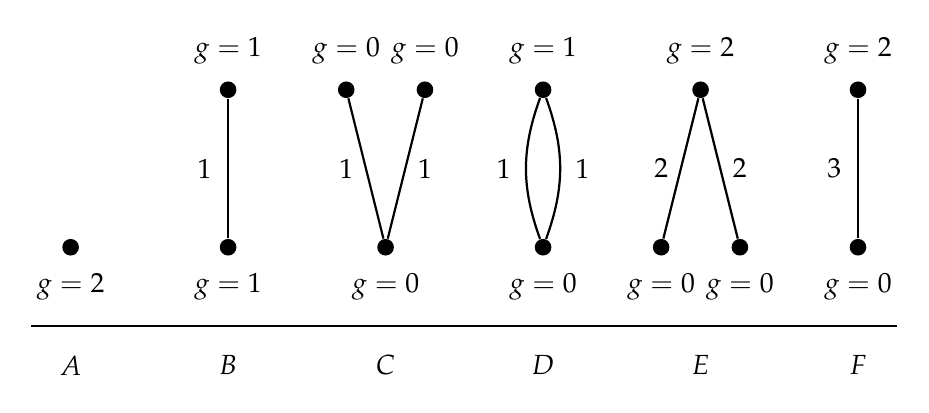
\begin{tikzpicture}[scale=1, transform shape]
        \node[fill=black,circle,minimum size=6pt,inner sep=0pt] (A) at (0,0) {};
        \node[fill=black,circle,minimum size=6pt,inner sep=0pt] (B1) at (2,0) {};
        \node[fill=black,circle,minimum size=6pt,inner sep=0pt] (B2) at (2,2) {};
        \node[fill=black,circle,minimum size=6pt,inner sep=0pt] (C1) at (4,0) {};
        \node[fill=black,circle,minimum size=6pt,inner sep=0pt] (C2) at (3.5,2) {};
        \node[fill=black,circle,minimum size=6pt,inner sep=0pt] (C3) at (4.5,2) {};
        \node[fill=black,circle,minimum size=6pt,inner sep=0pt] (D1) at (6,0) {};
        \node[fill=black,circle,minimum size=6pt,inner sep=0pt] (D2) at (6,2) {};
        \node[fill=black,circle,minimum size=6pt,inner sep=0pt] (E1) at (8,2) {};
        \node[fill=black,circle,minimum size=6pt,inner sep=0pt] (E2) at (7.5,0) {};
        \node[fill=black,circle,minimum size=6pt,inner sep=0pt] (E3) at (8.5,0) {};
        \node[fill=black,circle,minimum size=6pt,inner sep=0pt] (F1) at (10,0) {};
        \node[fill=black,circle,minimum size=6pt,inner sep=0pt] (F2) at (10,2) {};
        \draw[-,thick] (B1) -- (B2);
        \draw[-,thick] (C2) -- (C1) -- (C3);
        \draw[-,thick] (D1) edge[bend left=20] (D2);
        \draw[-,thick] (D2) edge[bend left=20] (D1);
        \draw[-,thick] (E2) -- (E1) -- (E3);
        \draw[-,thick] (F1) -- (F2);
        \node at (0,-0.5) {$g=2$};
        \node at (2,-0.5) {$g=1$};
        \node at (4,-0.5) {$g=0$};
        \node at (6,-0.5) {$g=0$};
        \node at (7.5,-0.5) {$g=0$};
        \node at (8.5,-0.5) {$g=0$};
        \node at (10,-0.5) {$g=0$};
        \node at (2,2.5) {$g=1$};
        \node at (3.5,2.5) {$g=0$};
        \node at (4.5,2.5) {$g=0$};
        \node at (6,2.5) {$g=1$};
        \node at (8,2.5) {$g=2$};
        \node at (10,2.5) {$g=2$};
        \draw[-,thick] (-0.5,-1) -- (10.5,-1);
        \node at (0,-1.5) {$A$};
        \node at (2,-1.5) {$B$};
        \node at (4,-1.5) {$C$};
        \node at (6,-1.5) {$D$};
        \node at (8,-1.5) {$E$};
        \node at (10,-1.5) {$F$};
        \node at (1.7,1) {$1$};
        \node at (3.5,1) {$1$};
        \node at (4.5,1) {$1$};
        \node at (5.5,1) {$1$};
        \node at (6.5,1) {$1$};
        \node at (7.5,1) {$2$};
        \node at (8.5,1) {$2$};
        \node at (9.7,1) {$3$};
    \end{tikzpicture}
    \end{center}
        \caption{$X = \mr{pt}$、\(Z = \emptyset\) 且 $g=2$ 时热带类型的图。}%
    \label{fig:tropgraphs}
    \end{figure}
\end{exm}

\begin{thm}[热带量子 Lefschetz {\cite{CJRtropical2025}}]
    设 \(X\) 与 \(Z\) 如前。对任意 \(\beta \in H_2(X)\)、任意 \(\alpha_1, \ldots, \alpha_n \in H^*(X)\) 以及任意 \(k_1, \ldots, k_n \in \N\)，我们有
    \begin{align*}
        \int_{[\bar{M}_{g,n}(Z,\beta)]^{\vir}} \prod_{j=1}^n \ev_j^* (\alpha_j) \psi^{k_j}={}& (-1)^{1-g+\beta \cdot Z} \cdot \sum_{\tau \vdash (g,n,\beta)} \frac{(-1)^{\abs{\V_{\infty}}}}{\abs{\Aut(\tau)}} \cdot \prod_{E \in \E} c(E) \\
        & \cdot \sum_{\ab\{j_E \mid E = \ab\{E_{\log}, E_{\infty}\}\}}  \prod_{v \in \V_{\infty}} \int_{[\mc{U}_v]^{\on{red}}} \prod_{E_{\infty} \in \H_v} \ev_{E_{\infty}}^* \phi^{j_E}  \\
        &  \cdot \prod_{v \in \V_{\log}} \int_{[\mc{R}_v]^{\vir}} \prod_{E_{\log}} \ev_{E_{\log}}^* (\phi_{j_E}) \cdot \prod_{h \in \L_v} \ev_h^* \alpha_h \cdot \psi_h^{k_h} .
    \end{align*}
\end{thm}

\begin{rmk}
    还有一个虚局部化公式（在~\cite{CJRlocalization}中预告），它既可以应用于约化理论（只带 R-环面作用），也可以应用于典范理论（可以应用于环境空间的全部自同构）。
\end{rmk}

现在考虑一个 \(\infty\)-顶点。令 \(\tau_v = (g, c, \beta)\)，并令 \(\mc{U}_v = \mc{U}_{g,c}(\infty, \beta)\)。则第一个计算是
\begin{align*}
    \on{red}\dim \mc{U}_v &= \chi(f^* T_{\mf{P}/B \C^{\times}_{\omega}}) + 1 + \on{trop}\dim  \\
    &= \vir\dim \bar{M}_{g,n}(Z, \beta) + \sum_{h \in \H } (c(h) + 1),
\end{align*}
其中热带维数为 \(3g-4+n\)。注意所有接触阶都是负的，故第二项至多为零。特别地，我们已证明
\begin{cor}[{\cite{CJRpunctured}}]
    若 \(\vir\dim \bar{M}_{g,n}(Z,\beta) < 0\)，则 \([\mc{U}_v]^{\on{red}} = 0\)。
\end{cor}
我们还有一个\textit{平衡条件}，它断言
\begin{equation}\label{eqn:balancing condition}
    \sum_{h \in \H} c(h) = \deg f^* \mc{O}(\infty) = \int_{\beta} c_1(V) - (2g-2+n).
\end{equation}
这可以改写为
\[ 0 \geq \sum_{h \in \H} (c(h)+1) = \int_{\beta} c_1(V) - (2g-2). \]
\begin{prop}[{\cite{CJRpunctured}}]
    我们看到在下列情形中 \(\infty\)-顶点不存在：
    \begin{enumerate}
        \item \(g = 0\) 且 \(V\) 是 nef 的；
        \item \(g=1\) 且 \(V\) 是丰富的，除非 \(\beta = 0\) 且所有 \(c(h) = -1\)。
    \end{enumerate}
\end{prop}

\begin{defn}
    一个标记称为\textit{单位}，如果其接触阶为 \(-1\)。
\end{defn}

\begin{notn}
    我们将单位扇区记作 \(\1\)，并记 \(\tau_{v+\1} = (g, c+\1, \beta)\)，\(\mc{U}_{v+\1} = \mc{U}_{g, c+\1}(\infty, \beta)\)，以及 \(\mc{R}_{v+\1} = \mc{R}_{g, c+\1}(\infty, \beta)\)。
\end{notn}

\begin{thm}[{\cite[定理~1.16--1.17]{CJRpunctured}}]\leavevmode
    \begin{enumerate}
        \item 存在一个映射 \(F_{\1} \colon \mc{U}_{v+\1} \xrightarrow{s} \mc{C}^{\circ} \xrightarrow{\pi} \mc{U}_v\)，其中 \(s\) 是双有理的；
        \item 约化虚闭链之间有等式 \(s_* [\mc{U}_{v+\1}]^{\on{red}} = \pi^* [\mc{U}_v]^{\on{red}}\)；
        \item 若 \(D\) 是 \(X\) 上的除子，则 \(F_{\1 *} (\ev_{\1}^* D \cap [\mc{U}_{v+\1}]^{\on{red}}) = \ab(\int_{\beta} D) [\mc{U}_v]^{\on{red}}\)；
        \item 考虑图
            \begin{equation*}
            \begin{tikzcd}
                \mc{U}_{v+\1} \ar{r}{F} \ar{d}[swap]{F_{\1}} & \bar{M}_{g,n+1} \ar{d}[swap]{p} \\
                \mc{U}_v \ar{r}{F} & \bar{M}_{g,n}.
            \end{tikzcd}
            \end{equation*}
            则 \(F_* [\mc{U}_{v+\1}]^{\on{red}} = p^* F_* [\mc{U}_v]^{\on{red}}\)。
    \end{enumerate}
\end{thm}

\begin{exm}
    考虑 \(g = 1\) 且 \(Z_d \subset X = \P^N\) 是超曲面的情形。我们只需考虑 \(\beta = 0\) 且对所有 \(h \in \H\) 有 \(c(h) = -1\) 的情形。于是我们看到
    \[ \prod_h \ev_h^* \alpha_h \cdot [\mc{U}_{1,c}(\infty,\beta)]^{\mr{red}} = \ev_{h^{\star}}^* \ab(\prod_h \alpha_h) \cap [\mc{U}_{1,\1}(\infty,\beta)]^{\on{red}}. \]
\end{exm}

\begin{prop}[{\cite{CJRpunctured}}]
    我们实际上有
    \[ \mc{U}_{1,\1}(\infty, 0) \simeq \mc{R}_{1,\1}(\infty, 0) \]
    以及等式
    \[ [\mc{U}_{1,\1}(\infty, 0)]^{\on{red}} = c_{\dim X} \ab(\mc{H}^{\vee} \boxtimes T_{\mf{P}/B\C_{\omega}^{\times}} + \mc{O} - V). \]
\end{prop}

\begin{exm}
    现在考虑五次三维流形 \(Z_5 \subset \P^4\)。我们看到 \(\on{red}\dim \mc{U}_v = \sum_{h \in \H} (c(h)+2)\)。单位公理把我们归结到 \(c(h) \leq -2\) 的情形。现在我们需要确定当所有 \(c(h) = -2\) 时需要考虑的新不变量的个数，这等价于求可能的 \(\beta\) 的个数。平衡条件断言
    \begin{align*}
        \sum_{h \in \H} c(h) &= \int_{\beta} c_1(V) - (2g-2+n) \\
        &= 5\beta - (2g-2+n),
    \end{align*}
    由此可知 \(0 \geq \sum (c(h)+1) = 5\beta - (2g-2)\)，因此 \(\beta \leq \frac{2g-2}{5}\)。\footnote{若假设有限生成、全纯反常方程、轨形正则性与锥形点间隙条件，这恰好是所预言的未知量个数。}
\end{exm}

\begin{conj}[Janda {\cite[猜想~1.6]{CJRtropical2025}}]\leavevmode
    \begin{enumerate}
        \item 我们有 \(K(Q) = \log I_0(q) \cdot c_1(K_X^{\vee}) - \frac{I_1}{I_0}\) \\
        \item 典范理论满足 \(\Omega \in I_0(q)^{2g-2+2n_1 + 3 n_2} \cdot R\)。
    \end{enumerate}
\end{conj}

\begin{cor}[{\cite[定理~1.7]{CJRtropical2025}}]
    上述关于 \((X, V)\) 的猜想蕴含 \(Z\) 的 Yamaguchi–丘成桐有限生成性。
\end{cor}


\section{五次三维流形高亏格 GW 不变量的结构（郭帅）}%
\label{sec:Structure of higher-genus GW invariants of the quintic (Shuai Guo)}

\subsection{问题}%
\label{sub:The problem (Guo)}

我们考虑五次三维流形\(X = X_5 \subset \P^4\)，并问它包含多少条亏格为\(g\)、次数为\(d\)的曲线。在亏格零，答案的开头是
\[ 2875, \qquad 609250, \qquad 317206375, \qquad \ldots \]

由于\(X\)是 Calabi-Yau 的，模空间\(\Mbar_{g,n}(X,\beta)\)的虚维数为零，并且弦方程给出：除非\((g,n,\beta) = (0,3,0)\)，否则\(\ab<\1, \gamma_2, \ldots, \gamma_n>_{g,n,\beta} = 0\)。因此我们定义初级不变量为
\[ N_{g,\beta} \coloneqq \ab<>_{g,0,\beta} = \int_{[\Mbar_g(X,\beta)]^{\vir}} 1 \]
并把这些数打包进生成级数
\[ F_g(Q) \coloneqq \sum_{\beta \text{有效}} N_{g,\beta}Q^{\beta}. \]

不变量\(N_{g,\beta}\)是有理数，而我们真正想要的整数是 BPS 不变量\(n_{g,\beta}\)。它们由正次数部分\(F_g^+\)通过多重覆盖变换定义：
\[ \sum_{g \geq 0} F_g^+(Q)\lambda^{2g-2} = \sum_{\substack{g \geq 0 \\ \beta > 0}} n_{g,\beta} \sum_{k \geq 1} \frac{1}{k} \ab(2 \sin \frac{k\lambda}{2})^{2g-2}Q^{k\beta}. \]
注意只有\(n_{g,\beta}\)被期望是整数，而上面的那些数是\(n_{0,d}\)。

\begin{table}[htpb]
    \centering
    \caption{五次三维流形的前几个 BPS 不变量\(n_{g,d}\)}
    \label{tab:quinticbps}
    \begin{tabular}{crrrrr}
        \toprule
        \(g\) & \(d=1\) & \(d=2\) & \(d=3\) & \(d=4\) & \(d=5\) \\
        \midrule
        0 & 2875 & 609250 & 317206375 & 242467530000 & 229305888887625 \\
        1 & 0 & 0 & 609250 & 3721431625 & 12129909700200 \\
        2 & 0 & 0 & 0 & 534750 & 75478987900 \\
        3 & 0 & 0 & 0 & 8625 & \(-15663750\) \\
        4 & 0 & 0 & 0 & 0 & 49250 \\
        5 & 0 & 0 & 0 & 0 & 1100 \\
        6 & 0 & 0 & 0 & 0 & 10 \\
        7 & 0 & 0 & 0 & 0 & 0 \\
        \bottomrule
    \end{tabular}
\end{table}

我们看到~\Cref{tab:quinticbps}的每一列最终都变为零。这就是 Castelnuovo 界，对五次三维流形它断言当\(g > \frac{d^2+5d+10}{10}\)时\(n_{g,d} = 0\)，由刘治宇–阮勇斌~\cite{LiuRuanCastelnuovo}证明。表中各项的整性是 Gopakumar-Vafa 猜想，由 Ionel-Parker~\cite{IonelParker2018}证明。

在亏格零，Candelas-de la Ossa-Green-Parkes 利用镜像上的周期积分计算了\(F_0\)，我们在~\Cref{sub:Enumerative mirror symmetry in genus zero}中讨论过。在高亏格，Bershadsky-Cecotti-Ooguri-Vafa 给出了一个递归，它由\(h < g\)的\(F_h\)产生\(F_g\)，至多相差有限多个未知常数。我们的目标是解释对数 GLSM 如何确定这一模糊性。

\subsection{亏格零与 B-模型的多项式结构}%
\label{sub:Genus zero and the polynomial structure of the B-model}

回忆~\Cref{sub:Enumerative mirror symmetry in genus zero}，对五次三维流形我们考虑\(I\)-函数
\[
    I(q,z) = z\sum_{d \geq 0} q^{H/z+d} \frac{\prod_{m=1}^{5d}(5H+mz)}{\prod_{m=1}^d (H+mz)^5} = I_0 z + I_1 H + I_2 \frac{H^2}{z} + I_3 \frac{H^3}{z^2},
\]
其各分量被 Picard-Fuchs 算子
\[ D^4 - 5q(5D+1)(5D+2)(5D+3)(5D+4), \qquad D = q \odv{}{q}. \]
零化。若记\(J_k = I_k/I_0\)以及\(\frac{I_1}{I_0} = \log q + \tau(q)\)，从而\(Q = e^{I_1/I_0} = qe^{\tau(q)} = q + O(q^2)\)，则亏格零镜像定理断言
\[ F_0(Q) = \frac{5}{2}\ab(J_1 J_2 - J_3). \]

为了我们的目的，把五次三维流形的公式放进一般的镜像对称图景中是有用的。设\(\mc{X} = \ab\{(X,\omega)\}\)是一族 Calabi-Yau 三维流形，其 Kähler 模为\(\mc{M} \ni Q = e^{2\pi i \omega}\)；设\(\mc{X}^{\vee} = \ab\{(X^{\vee},J)\}\)是一个镜像族，其复模为\(\mc{M}^{\vee} \ni q\)。Picard-Fuchs 方程的解是\(X^{\vee}\)上的周期，并组装成
\[ I(z) = zI_0\varphi_0 + I_1 + I_2 z^{-1} + I_3 z^{-2}, \]
它落在\(z\varphi_0, \varphi_{\alpha}, \varphi^{\alpha}z^{-1}, \varphi^0 z^{-2}\)张成的空间中。这里\(I_1 = \sum_{\alpha} I_1^{\alpha}\varphi_{\alpha}\)，\(I_2 = \sum_{\alpha} I_{2,\alpha}\varphi^{\alpha}\)，\(I_3 = I_{3,0}\varphi^0\)，而镜映射仍为\(Q = e^{I_1/I_0} = qe^{\tau(q)}\)。

我们将用到五次三维流形复模直线上的三个特殊点：大复结构点\(q=0\)、锥形点\(q = 5^{-5}\)（此处有一个周期为零）以及轨形点（或 Landau-Ginzburg 点）\(q = \infty\)。镜映射在\(q=0\)处有定义，在那里的展开给出 Gromov-Witten 不变量，而在高亏格我们将在另外两个点处施加边界条件。

现在我们用三点函数重述镜像定理。在\(\mc{M}^{\vee}\)上取局部坐标\(q_i\)，设\(\ab\{\phi_i\}\)是 A-侧对应的基，并定义
\[ C^A_{ijk}(Q) \coloneqq I_0^2 \ab<\phi_i, \phi_j, \phi_k>^X_{0,3}, \qquad C^B_{ijk}(q) \coloneqq \int_{X^{\vee}} \partial_i \partial_j \partial_k \Omega \wedge \Omega. \]

\begin{thm}[镜像定理 {\cite{Givental1998,LLY1997}}]
    我们有\(C^A_{ijk}(Q(q)) = C^B_{ijk}(q)\)。此外\(C^B_{ijk} \in \Delta^{-1}\Q[q]\)，因此它是\(\mc{M}^{\vee}\)上整体定义的亚纯函数，极点只沿判别式出现。
\end{thm}

特别地，乘以\(I_0\)的适当幂次并应用镜映射之后，一个亏格零生成函数就变成\(q\)的有理函数，极点只沿判别式出现。因此，它由有限多个系数确定。

\begin{exm}
    对五次三维流形，在超平面基下，
    \[ C_{111} = \frac{5}{1-5^5 q}. \]
\end{exm}

\begin{exm}
    对\(X = X_{3,3} \subset \P^2 \times \P^2\)，Yukawa 耦合为
    \begin{align*}
        C_{111} &= \frac{3^4 q_1 (2+3^3q_1+3^3q_2)}{\Delta}, & C_{222} &= \frac{3^4 q_2(2+3^3q_1+3^3q_2)}{\Delta}, \\
        C_{112} &= \frac{(1-3^3q_1-3^3q_2)(1+2\cdot 3^3 q_1 - 3^3 q_2)}{\Delta}, \\
        C_{122} &= \frac{(1-3^3q_1-3^3q_2)(1-3^3q_1+2\cdot3^3q_2)}{\Delta},
    \end{align*}
    其中
    \[ \Delta = 1 - 3\cdot3^3(q_1+q_2) + 3\cdot3^6(q_1^2 - 7q_1q_2+q_2^2) - 3^9(q_1+q_2)^3. \]
\end{exm}

在高亏格，我们期望有规范化势\(f^A_{g,i}\)满足
\[ f^A_{g,i}(Q(q)) = f^B_{g,i}(q) \in \Delta^{-(2g-2+n)}\Q[q], \]
其中右边由一个图求和计算。

\subsection{BCOV Feynman 规则}%
\label{sub:The BCOV Feynman rule}

B-模型的 Feynman 规则与全纯反常方程源自~\cite{BCOV1994}。对五次三维流形，张怀良–郭帅–李骏在~\cite{CGL2021}中证明了多项式性，并在~\cite{CGL2026}中证明了 Feynman 规则。

现在我们把 BCOV 递归作为一个 Feynman 规则来讨论。它来自~\Cref{sub:Operator formalism and geometric quantization}中辛变换量子化的一个有限维模型。设\(\mc{H} = \mc{H}^- \oplus \mc{H}^+ \subset \mc{H}_{\infty}\)是辛的，\(d+1 = \dim \mc{H}^+ = \dim \mc{H}^-\)，并令
\[ R = \begin{pmatrix} A & B \\ C & D \end{pmatrix} \in \End \mc{H}, \qquad \mc{Q}(\mbf{x},\bp) = (\bp, D^{-1}\mbf{x}) - \frac{1}{2}(\bp, D^{-1}C\bp). \]
给定总势\(F(\hbar, \mbf{x})\)，我们通过 Gauss 积分形式地定义变换后的势为
\[ f(\hbar, \mbf{x}) \coloneqq (\wh{R}F)(\hbar,\mbf{x}) = \ln \int e^{\hbar^{-1}(\mc{Q}(\mbf{x},\bp') - \mbf{x}'\bp') + F(\hbar,\mbf{x}')}\d{\mbf{x}'}\d{\bp'}. \]
按稳相展开就得到一个图求和。这里\(D^{-1}C\)提供每条边上的传播子，而\(F\)提供顶点。

对 Calabi-Yau 三维流形，传播子按指标个数记作\(S^{\varphi\varphi}\)、\(S^{\varphi}\)和\(S\)，顶点则是规范化的 A-模型关联函数
\[ P^A_{g,n}(Q) = I_0^{2-2g}\ab<\phi_1, \ldots, \phi_n>^X_{g,n}. \]
注意这些与后面将出现的、求解量子微分方程的算子\(S_{\tau}(z)\)毫无关系。

\begin{exm}
    对五次三维流形，在亏格二无标记点的情形，Feynman 规则写作
    \begin{align*}
        f_2^B ={}& P_2 + \frac{1}{2}S^{\varphi\varphi}P_{1,1}^2 + \frac{1}{2}S^{\varphi\varphi}P_{1,2} + (S^{\varphi\varphi})^2 P_{1,1} + \frac{1}{8}(S^{\varphi\varphi})^2 P_{0,4} \\
        &+ \frac{1}{8}(S^{\varphi\varphi})^3 + \frac{1}{12}(S^{\varphi\varphi})^3 + \frac{\chi}{24}S^{\varphi}P_{1,1} + \frac{1}{2}\frac{\chi}{24}S^{\varphi}S^{\varphi\varphi} \\
        &+ \frac{1}{2}\frac{\chi}{24}\ab(\frac{\chi}{24}-1)S,
    \end{align*}
    其中\(\chi = \chi(X_5) = -200\)。这是传播子的一个三次多项式。
\end{exm}

我们可以像~\Cref{sub:R-matrix action}那样把它解释为对稳定图的求和。顶点\(v\)贡献低亏格关联函数\(P_{g_v, \on{val}(v)}\)；内部边把两个插入与一个传播子缩并；腿记录剩余的插入。每个图带有权重\(\frac{1}{\ab|\Aut \Gamma|}\)。像通常一样，
\[ g(\Gamma) = h^1(\Gamma) + \sum_v g_v, \qquad 2g_v - 2 + \on{val}(v) > 0, \]
而\(f_g^B\)是所有亏格\(g\)稳定图贡献之和。

\subsection{全纯反常方程}%
\label{sub:The holomorphic anomaly equation}

现在我们把这个递归改写为一个微分方程。B-模型振幅\(\mc{F}_g(z,\bar{z})\)并非全纯，对\(g \geq 2\)，其非全纯性由下式给出：
\[ \partial_{\bar{i}} \mc{F}_g = \frac{1}{2}\bar{C}_{\bar{i}}^{jk}\ab( D_j D_k \mc{F}_{g-1} + \sum_{r=1}^{g-1} D_j \mc{F}_r D_k \mc{F}_{g-r} ). \]
这里\(C_{ijk}\)是 Yukawa 耦合，\(\bar{C}_{\bar{i}}^{jk}\)由\(\bar{C}_{\bar{i}\bar{j}\bar{k}}\)用 Weil-Petersson 度量升两个指标得到，\(D_j\)是 Hodge 线丛适当幂次上的协变导数。右边两项对应\(\Mbar_g\)的两个边界层，即非分离结点与分离结点。系数\(\frac{1}{2}\)忘掉了两个分支的顺序。

若我们选取局部\(\bar{\partial}\)-原函数
\[ \partial_{\bar{i}}S^{jk} = \bar{C}_{\bar{i}}^{jk}, \qquad \partial_{\bar{i}}S^j = G_{i\bar{\ell}}S^{\ell j}, \qquad \partial_{\bar{i}}S = G_{i\bar{\ell}}S^{\ell}, \]
那么在相差一个全纯项的意义下，反常方程变为多项式偏微分方程
\[ \pdv{\mc{F}_g}{S^{jk}} = \frac{1}{2}\ab( D_jD_k \mc{F}_{g-1} + \sum_{r=1}^{g-1} D_j \mc{F}_r D_k \mc{F}_{g-r} ). \]
这些传播子只在相差全纯张量的意义下有定义，这一自由度正是全纯模糊性的来源。

\begin{rmk}
    在我们将对五次三维流形使用的单参数规范化变量下，这写作
    \[ -\partial_0 P_g = \frac{1}{2}P_{g-1,2} + \frac{1}{2}\sum_{r=1}^{g-1}P_{r,1}P_{g-r,1}, \qquad -\partial_1 P_g = 0. \]
\end{rmk}

为了看出图求和为何满足这个方程，注意在无标记点的势中，非全纯生成元只出现在边因子里。因此沿传播子方向求导会挑出一条边并把它切开。两条半边成为所得低亏格顶点上的标记点，而由除子方程，协变导数正对应于这些标记点。切开一个圈得到\(P_{g-1,2}\)，切开一条分离边得到\(P_{g_1,1}P_{g_2,1}\)。

\begin{rmk}
    为清楚起见，这个推出关系只是单向的。BCOV 图规则蕴含反常方程，但反常方程本身并不确定图规则。要恢复同一个解，我们还需要传播子约定、低亏格顶点数据以及边界条件。
\end{rmk}

若所有低亏格顶点均已知，则右边已知，于是我们可以对非全纯生成元积分得到
\[ P_g = P_g^{\mr{particular}} + f_g(Y), \]
其中有限生成给出全纯模糊性
\[ f_g(Y) = P_g|_{A = B_1 = B_2 = B_3 = 0} = \sum_{i=0}^{3g-3}a_{i,g}Y^i, \qquad Y = (1-5^5q)^{-1}. \]
我们看到反常方程在每个亏格留下\(3g-2\)个未知系数。

\begin{rmk}
    对五次三维流形，零次数数据连同轨形正则性去掉其中\(\ceil{\frac{3g-3}{5}}+1\)个自由度，锥形点间隙又提供\(2g-2\)个条件，从而剩下
    \[ 3g-2 - \ab(\ceil*{\frac{3g-3}{5}}+1) - (2g-2) = \floor*{\frac{2g-2}{5}} \]
    个参数，它们是真正新的有效不变量。这恰好是~\Cref{eqn:balancing condition}所预测的\(\infty\)-顶点未知量的个数，即满足\(\beta \leq \frac{2g-2}{5}\)的\(\beta\)的个数。
\end{rmk}

于是我们得到物理学家提出的下述猜想性算法：BCOV Feynman 规则、Landau-Ginzburg 点处的轨形正则性（LG/CY 对应的一种形式，对五次三维流形这是郭帅–阮勇斌–Janda 正在进行的工作）以及锥形点间隙条件。在这些之外我们还可以加上 Gopakumar-Vafa 整性和 Castelnuovo 界。

\subsection{四个理论}%
\label{sub:Four theories}

回忆~\Cref{sec:Log GLSM (Qile Chen)}，对数 GLSM 带有两个虚闭链。约化闭链恢复五次三维流形的 Gromov-Witten 理论，而典范等变闭链容许一个单位根特殊化，它是半单的，因而可由 Givental-Teleman 计算。二部图求和
\[ \Omega^{\mr{GW}}_{g,n} = \sum_{\Gamma \text{二部}} \frac{1}{\ab|\Aut \Gamma|} \ab( \prod_{v \in V_{\infty}(\Gamma)} c^{\mr{eff}}_{g_v,\beta_v}) \Cont^{\mr{can}}_{\Gamma} \]
用后者表达前者，代价是在\(\infty\)-顶点处引入有效不变量\(c^{\mr{eff}}_{g,\beta}\)。把它们换成形式参数\(\mbf{C} = \ab\{c_{g,\beta}\}\)就得到\textit{扩张\(\mbf{C}\)-族}，其顶点数据由亚纯与橡皮对数 GLSM 理论提供。

我们将考虑下面四个理论。
\begin{itemize}
    \item \textit{\(t\)-扭几何理论}令\(\lambda_i = 0\)并保留辅助权\(t\)。它有稳定映射和稳定商两个版本，其中稳定商版本给出下面的亏格二局部化公式。
    \item \textit{形式五次}，即形式\(\lambda\)-扭理论，令\(t = 0\)且\(\lambda_i = \zeta_5^i \lambda\)。它是一个半单 CohFT，因此有一个普适且可计算的\(R\)-矩阵。
    \item \textit{扩张\(\mbf{C}\)-族}在这两者之间插值，也是同时含有形式顶点与亚纯顶点的二部图所在之处。
    \item \textit{五次三维流形 Gromov-Witten 理论}由令\(\mbf{C} = \mbf{C}^{\mr{eff}}\)再取\(\lambda \to 0\)得到，是我们想要计算的理论。
\end{itemize}

\begin{warn}
    在高亏格，\(t\)-扭稳定商理论的\(t^0\)系数并不是形式\(\lambda\)-扭理论的\(\lambda^0\)系数。
\end{warn}

\subsection{形式五次}%
\label{sub:The formal quintic}

形式五次及其全纯反常方程在~\cite{LhoPandharipande2019}中研究；与扩张理论的比较建立于~\cite{GJRstructure}。

设\(E = \mc{O}_{\P^4}(5)\)，并设\(\pi \colon \mc{C} \to \Mbar_{g,n}(\P^4,d)\)是泛曲线。\(t\)-扭闭链为
\[ e(R\pi_* f^* E \otimes [1]) \cap [\Mbar_{g,n}(\P^4,d)]^{\vir}, \]
其中\([1]\)的等变第一陈类为\(t\)。若改为从完全\((\C^{\times})^5\)-等变闭链出发，则形式五次是单位根特殊化
\[ [\Mbar_{g,n}(\P^4,d)]^{\vir,\lambda} \coloneqq \ab( e(R\pi_*f^*E \otimes [1]) \cap [\Mbar_{g,n}(\P^4,d)]^{\vir}_{(\C^{\times})^5})\Big|_{t=0, \; \lambda_i = \zeta_5^i \lambda}, \]
其中\(\zeta_5 = e^{2\pi i/5}\)。关系\(H^5 = \lambda^5\)使量子乘积一般地半单，同时把\(\lambda\)保留为一个参数。

状态空间、单位和配对由下式给出：
\[ \mc{H}_{\lambda} = \Q(\lambda)[H]/(H^5-\lambda^5), \quad \1 = 1, \quad (\gamma_1,\gamma_2)^{\lambda} = \int_{\P^4, (\C^{\times})^5} e(\mc{O}(5))\gamma_1\gamma_2 \Big|_{\lambda_i = \zeta_5^i\lambda}, \]
而 CohFT 类为
\[ \Omega^{\lambda}_{g,n}(\gamma_1, \ldots, \gamma_n) = \sum_{d \geq 0} q^d \rho_* \ab( \prod_{i=1}^n \ev_i^*(\gamma_i) \cap [\Mbar_{g,n}(\P^4,d)]^{\vir,\lambda}), \]
其中\(\rho\)忘掉映射并稳定化定义域。若用\(\tau(q)H\)平移，其中\(\tau(q) = I^{\lambda}_1(q)/I^{\lambda}_0(q)\)，则平移后的理论\(\Omega^{\lambda,\tau}\)是半单的。把标量扩张到\(\Q(\zeta_5,\lambda)\)之后，幂等基满足
\[ \omega^{\lambda}_{g,n}(e_{\alpha_1}, \ldots, e_{\alpha_n}) = \sum_{\alpha}\Delta_{\alpha}^{g-1}\prod_i \delta_{\alpha,\alpha_i}. \]
于是~\Cref{thm:teleman}给出
\[ \Omega^{\lambda,\tau}_{g,n} = \sum_{\Gamma \in G_{g,n}} \frac{1}{\ab|\Aut\Gamma|}\iota_* \Cont_{\Gamma} \]
其装饰如~\Cref{sub:R-matrix action}所述。带有\(\gamma\)的腿得到\(R^{-1}(\bar{\psi})\gamma\)，边得到
\[ V_R(z_1,z_2) = \frac{\sum_{\alpha} e_{\alpha}\otimes e^{\alpha} - \sum_{\alpha} R^{-1}(z_1)e_{\alpha} \otimes R^{-1}(z_2)e^{\alpha}}{z_1+z_2}, \]
顶点得到拓扑场论\(\omega\)，而缺失的保单位部分通过\(T(z) = z(\1 - R^{-1}(z)\1)\)插入在被忘却的标记点处。

\begin{rmk}
    我们看到边因子没有极点。令\(z_2 = -z_1\)并用形如\(R^{-1}(z) = R^*(-z)\)的辛条件，分子为零。因此它能被\(z_1+z_2\)整除，\(V_R\)是两个余切线变量的幂级数。\(z_1^p z_2^q\)的系数是放在结点处带有\(\bar{\psi}_1^p \bar{\psi}_2^q\)的类，把它与相邻的两个拓扑场论张量缩并就把两个分支粘合起来。
\end{rmk}

\subsection{如何计算\(R\)-矩阵}%
\label{sub:How to compute the R-matrix (Guo)}

为了计算\(R\)-矩阵，我们从形式等变\(I\)-函数出发：
\[ I^{\lambda}(q,z) = z\sum_{d\geq0}q^d \frac{\prod_{m=1}^{5d}(5H+mz)}{\prod_{m=1}^d ((H+mz)^5 - \lambda^5)} = zI_0 + I_1^{\lambda}H + z^{-1}I_2^{\lambda}H^2 + \cdots. \]
直到\(H\)的系数与\(\lambda\)无关，因此\(I_1^{\lambda} = I_1 - I_0 \log q\)，而镜像平移\(\tau(q) = I_1^{\lambda}(q)/I_0(q)\)不含对数。令
\[ D = q\odv{}{q}, \qquad Y = (1-5^5q)^{-1}, \qquad L = Y^{1/5} \]
并引入基
\[ \phi_k = I_{1,1}\cdots I_{k,k}H^k, \qquad \bar{\phi}_k = I_0 L^{-k-1}\phi_k, \]
其中对角 Birkhoff 因子由下式递归定义：
\[ I_{p,0} = I_p, \qquad I_{p,r} = \frac{I_{p-1,r-1}}{I_{r-1,r-1}} + D \ab( \frac{I_{p,r-1}}{I_{r-1,r-1}}), \quad 1 \leq r \leq p, \]
特别地\(I_{1,1} = 1+D\tau\)。幂等元与典范坐标由下式给出：
\[ e_{\alpha} = \frac{1}{5}\sum_{i=0}^4 h_{\alpha}^{-i}\frac{\phi_i}{L^i}, \qquad u_{\alpha} = h_{\alpha}\int_0^q (L(s)-1)\frac{\d{s}}{s}, \qquad h_{\alpha} = \zeta_5^{\alpha}\lambda. \]

我们将用量子微分方程来确定\(R\)-矩阵对\(q\)的依赖。基本解满足
\[ zDS_{\tau}(z) + S_{\tau}(z)H = M_{\tau}S_{\tau}(z), \qquad M_{\tau} = \dot{\tau}\star, \quad \dot{\tau} \coloneqq (1+D\tau)H = I_{1,1}H, \]
而在规范化典范方向\(\alpha\)上，稳相渐近给出
\[ (S_{\tau})_{i\bar{\alpha}}(z)C_{\alpha}(z)^{-1} = e^{u_{\alpha}/z}R_{i\bar{\alpha}}(z), \]
从而
\[ (zD+h_{\alpha}L)R_{i\bar{\alpha}} = \sum_j (M_{\tau})_i^j R_{j\bar{\alpha}}. \]
这里\(C_{\alpha}(z)\)是\(q=0\)处的量子 Riemann-Roch（等价地，Γ-函数）因子，它连同辛条件一起固定了微分方程看不到的那些常数。与~\Cref{sub:How to compute the R-matrix}末尾一样，微分方程给出一个递归，而振荡积分给出初始条件。

记\(R(z) = \mr{Id} + R_1 z + R_2 z^2 + \cdots\)，我们可以用上面的方程由前面各项确定每个\(R_{k+1}\)。有两个特点使五次三维流形的情形变得可处理。第一，单位根基有五个扇区，一个模\(5\)的荷规则使每一行只允许一种留数模式。于是在任何计算开始之前，大多数矩阵元就已为零。第二，每个系数都落在有限生成环
\[ \mc{R} = \Q[A,B_1,B_2,B_3,Y], \qquad A = \frac{DI_{1,1}}{I_{1,1}}, \quad B_k = \frac{D^k I_0}{I_0}, \]
中，因此稳定图求和归结为一个有限的代数计算。

\begin{rmk}
    特别地，由于维数原因，固定的亏格只需要\(R\)的有限多项。在\(\Mbar_{g,n}\)上只有总次数至多为\(3g-3+n\)的类有贡献，其余全部积分为零，因此对无标记点的势我们只需要\(R_0, \ldots, R_{3g-3}\)。亏格\(4\)止于\(z^9\)，亏格\(5\)止于\(z^{12}\)。
\end{rmk}

\subsection{亏格二}%
\label{sub:Genus two}

这里讨论的亏格二镜像公式归功于郭帅–Janda–阮勇斌~\cite{GJRgenus2}。

现在我们在亏格二把两条路线都走一遍。几何路线使用\(t\)-扭稳定商理论，应用虚局部化得到五个贡献，然后应用稳定商穿墙落到五次三维流形的 Gromov-Witten 理论上。形式路线使用半单的\(\lambda\)-扭理论和\(R\)-矩阵来计算一个稳定图求和。这只给出形式主导部分。然后还必须加上有效的与亚纯的剩余图。

\begin{notn}
    记
    \[ \ab<\alpha_1, \ldots, \alpha_n>^{t,\mr{SQ}}_{g,n} \coloneqq \sum_{d\geq0}q^d \int_{[\Mbar_{g,n}(\P^4,d)]^{\vir}}e(R\pi_*\mc{L}^{\otimes 5}\otimes[-1])\prod_i \ev_i^*(\alpha_i), \]
    其中\(\mc{L}\)是泛稳定商线丛，且\(c_1^{\C^{\times}}([-1]) = -t\)（下面我们会回到这一符号约定）。这是稳定商的符号约定，与上面稳定映射闭链中出现的\([1]\)不同。
\end{notn}

\begin{figure}[htpb]
    \centering
    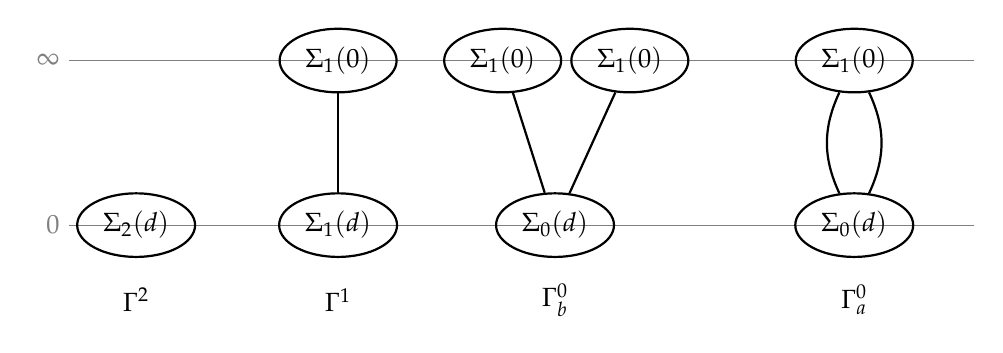
\begin{tikzpicture}[scale=0.95,transform shape]
        \draw[gray] (-0.9,0) -- (11.2,0);
        \draw[gray] (-0.9,2.2) -- (11.2,2.2);
        \node[anchor=east,gray] at (-0.9,0) {$0$};
        \node[anchor=east,gray] at (-0.9,2.2) {$\infty$};
        \node[ellipse,draw,thick,minimum width=1.5cm,minimum height=0.75cm] (a) at (0,0) {$\Sigma_2(d)$};
        \node at (0,-1) {$\Gamma^2$};
        \node[ellipse,draw,thick,minimum width=1.5cm,minimum height=0.75cm] (b0) at (2.7,0) {$\Sigma_1(d)$};
        \node[ellipse,draw,thick,minimum width=1.5cm,minimum height=0.75cm] (b1) at (2.7,2.2) {$\Sigma_1(0)$};
        \draw[thick] (b0) -- (b1);
        \node at (2.7,-1) {$\Gamma^1$};
        \node[ellipse,draw,thick,minimum width=1.5cm,minimum height=0.75cm] (c0) at (5.6,0) {$\Sigma_0(d)$};
        \node[ellipse,draw,thick,minimum width=1.5cm,minimum height=0.75cm] (c1) at (4.9,2.2) {$\Sigma_1(0)$};
        \node[ellipse,draw,thick,minimum width=1.5cm,minimum height=0.75cm] (c2) at (6.6,2.2) {$\Sigma_1(0)$};
        \draw[thick] (c0) -- (c1);
        \draw[thick] (c0) -- (c2);
        \node at (5.6,-1) {$\Gamma_b^0$};
        \node[ellipse,draw,thick,minimum width=1.5cm,minimum height=0.75cm] (d0) at (9.6,0) {$\Sigma_0(d)$};
        \node[ellipse,draw,thick,minimum width=1.5cm,minimum height=0.75cm] (d1) at (9.6,2.2) {$\Sigma_1(0)$};
        \draw[thick] (d0) to[bend left=25] (d1);
        \draw[thick] (d0) to[bend right=25] (d1);
        \node at (9.6,-1) {$\Gamma_a^0$};
    \end{tikzpicture}
    \caption{亏格二的四个非常值局部化图，每个顶点画成其对应的 Riemann 面分支。}%
    \label{fig:g2loc}
\end{figure}

四个非常值图画在~\Cref{fig:g2loc}中，它们的贡献为
\begin{align*}
    \Cont_{\Gamma^2} &= \ab<>^{t,\mr{SQ}}_{2,0}, \\
    \Cont_{\Gamma^1} &= -\ab< \frac{-\frac{5}{2}H^3 + \frac{5}{24}H^4t^{-1}}{(t-5H)(t-5H-\psi)}>^{t,\mr{SQ}}_{1,1}, \\
    \Cont_{\Gamma_b^0} &= \ab< \frac{-\frac{5}{2}H^3+\frac{5}{24}H^4t^{-1}}{(t-5H)(t-5H-\psi_1)}, \frac{-\frac{5}{2}H^3+\frac{5}{24}H^4t^{-1}}{(t-5H)(t-5H-\psi_2)}>^{t,\mr{SQ}}_{0,2},
\end{align*}
而对双边图，记\(H_1 = H \otimes 1\)和\(H_2 = 1 \otimes H\)，则
\[ \Cont_{\Gamma_a^0} = \ab< \frac{\frac{5}{3}(H^3\otimes H^4 + H^4 \otimes H^3)t^{-1} + \frac{65}{24}H^4 \otimes H^4 t^{-2}}{(t-5H_1)(t-5H_1-\psi_1)(t-5H_2)(t-5H_2-\psi_2)}>^{t,\mr{SQ}}_{0,2}. \]
注意这些关联函数生活在\(\P^4\)上，所以\(H^4\)存在且非零。

还有来自零次数图的第五个贡献，它是常数
\[ -2c_{2,0} = -\frac{5}{144}, \qquad c_{2,0} = -\frac{1}{2}N_{2,0} = \frac{5}{288}, \]
把五个贡献相加，我们得到局部化恒等式
\[ F_2^{\mr{SQ}}(q) = \Cont_{\Gamma^2} + \Cont_{\Gamma^1} + \frac{1}{2}\Cont_{\Gamma_a^0} + \frac{1}{2}\Cont_{\Gamma_b^0} - 2c_{2,0}, \]
其中两个因子\(\frac{1}{2}\)来自\(\Gamma_a^0\)与\(\Gamma_b^0\)的自同构。

令\(Q = qe^{\tau(q)}\)和\(L = (1-5^5q)^{-1/5}\)，其中\(\tau(q) = I_1(q)/I_0(q) - \log q\)是通常的镜像平移。现在我们应用稳定商穿墙得到精确恒等式
\[ F_2^{\mr{GW}}(Q) = I_0(q)^2 F_2^{\mr{SQ}}(q). \]
引入\(D_u = L^{-1}q\odv{}{q}\)以及生成元
\[ \mc{X}_k = D_u^k \log \frac{I_0}{L}, \qquad \mc{Y}_k = D_u^k \log \frac{I_0I_{1,1}}{L^2}, \qquad I_{1,1} = 1 + q \odv{\tau}{q}, \quad D_u L = \frac{1}{5}(L^5-1), \]
各个扭图的贡献单独来看会涉及额外的生成元。对我们而言重要的一点是，这些额外生成元在上述线性组合中相互抵消，恰好只剩下有限生成变量。记\(X = \mc{X}_1\)和\(Y_1 = \mc{Y}_1\)，我们得到
\begin{align*}
    F^{\mr{GW}}_2(Q) = \frac{I_0^2}{L^2}\Big(&\frac{70}{9}\mc{X}_3 + \frac{575}{18}X\mc{X}_2 + \frac{557}{72}X^3 + \frac{5}{6}Y_1\mc{X}_2 \\
    &- \frac{629}{72}Y_1X^2 - \frac{23}{24}Y_1^2 X - \frac{1}{24}Y_1^3 \\
    &+ \frac{125}{36}\mc{X}_2 L^4 - \frac{5}{24}X^2L^4 - \frac{35}{9}Y_1XL^4 - \frac{5}{24}Y_1^2L^4 \\
    &- \frac{1441}{300}XL^3 - \frac{41}{300}Y_1L^3 + \frac{31459}{7200}XL^8 + \frac{2141}{7200}Y_1L^8 \\
    &+ \frac{29621}{12000}L^{12} - \frac{116369}{36000}L^7 + \frac{547}{750}L^2\Big).
\end{align*}
若在大半径处展开，则得到
\[ F_2^{\mr{GW}}(Q) = -\frac{5}{144} + \frac{575}{48}Q + \frac{5125}{2}Q^2 + \frac{7930375}{6}Q^3 + O(Q^4), \]
这些系数是 Gromov-Witten 不变量\(N_{2,d}\)，而不是~\Cref{tab:quinticbps}中的 BPS 整数。

现在转向形式路线。\(\Omega^{\lambda}_{2,0}\)的 Givental-Teleman 公式是对亏格二无腿的七个稳定图的求和，它们画在~\Cref{fig:g2stable}中。只需要\(R^{-1}(z)\)直到\(z^3\)的部分，而平移把七种拓扑展开为\(17\)个装饰层。

\begin{figure}[htpb]
    \centering
    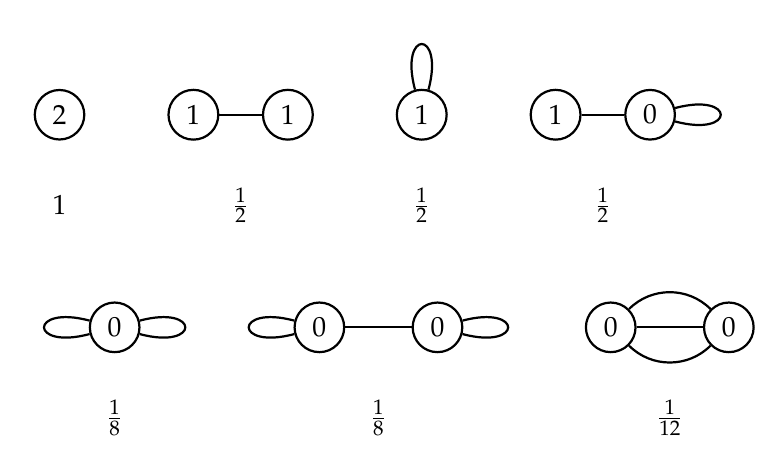
\begin{tikzpicture}[scale=1,transform shape,every loop/.style={min distance=8mm,looseness=10}]
        \node[circle,draw=black,thick] (a) at (0,0) {$2$};
        \node at (0,-1.15) {$1$};

        \node[circle,draw=black,thick] (b1) at (1.7,0) {$1$};
        \node[circle,draw=black,thick] (b2) at (2.9,0) {$1$};
        \draw[thick] (b1) -- (b2);
        \node at (2.3,-1.15) {$\frac{1}{2}$};

        \node[circle,draw=black,thick] (c) at (4.6,0) {$1$};
        \draw[thick] (c) edge[loop above] (c);
        \node at (4.6,-1.15) {$\frac{1}{2}$};

        \node[circle,draw=black,thick] (d1) at (6.3,0) {$1$};
        \node[circle,draw=black,thick] (d2) at (7.5,0) {$0$};
        \draw[thick] (d1) -- (d2);
        \draw[thick] (d2) edge[loop right] (d2);
        \node at (6.9,-1.15) {$\frac{1}{2}$};

        \node[circle,draw=black,thick] (e) at (0.7,-2.7) {$0$};
        \draw[thick] (e) edge[loop left] (e);
        \draw[thick] (e) edge[loop right] (e);
        \node at (0.7,-3.85) {$\frac{1}{8}$};

        \node[circle,draw=black,thick] (f1) at (3.3,-2.7) {$0$};
        \node[circle,draw=black,thick] (f2) at (4.8,-2.7) {$0$};
        \draw[thick] (f1) -- (f2);
        \draw[thick] (f1) edge[loop left] (f1);
        \draw[thick] (f2) edge[loop right] (f2);
        \node at (4.05,-3.85) {$\frac{1}{8}$};

        \node[circle,draw=black,thick] (g1) at (7.0,-2.7) {$0$};
        \node[circle,draw=black,thick] (g2) at (8.5,-2.7) {$0$};
        \draw[thick] (g1) -- (g2);
        \draw[thick] (g1) to[bend left=45] (g2);
        \draw[thick] (g1) to[bend right=45] (g2);
        \node at (7.75,-3.85) {$\frac{1}{12}$};
    \end{tikzpicture}
    \caption{亏格二无腿的七个稳定图，以顶点的亏格标记，并以\(\frac{1}{\ab|\Aut\Gamma|}\)加权。幻灯片上每个顶点画成其对应的 Riemann 面分支。}%
    \label{fig:g2stable}
\end{figure}

\begin{rmk}
    这些是稳定曲线的对偶图，而不是~\Cref{fig:tropgraphs}中的图，后者是把热带分解公式应用于对数 GLSM 的约化理论所得到的刚性热带类型。这两组拓扑在此恰好重合，但顶点在两处的含义不同。这里顶点是定义域曲线上带有拓扑场论张量的一个分支。那里顶点是二部热带曲线的一个水平，带有对数模问题或\(\infty\)-顶点模问题。
\end{rmk}

对形式路线，我们内蕴地定义规范化势为
\[ P_2^{\lambda} \coloneqq \frac{Y}{I_0^2}F_2^{\lambda}, \qquad Y = L^5. \]
完整的图求和落在\(\Q[L,\mc{X}_1,\mc{X}_2,\mc{X}_3,\mc{Y}_1]\)中，且等于
\begin{align*}
    P_2^{\lambda} ={}& -\frac{1}{128}L^{12} - \frac{23}{960}L^8\mc{X}_1 - \frac{9}{640}L^8\mc{Y}_1 + \frac{109}{16000}L^7 \\
    &- \frac{3}{80}L^4\mc{X}_1^2 - \frac{19}{320}L^4\mc{X}_1\mc{Y}_1 - \frac{3}{80}L^4\mc{Y}_1^2 - \frac{1}{64}L^4\mc{X}_2 \\
    &+ \frac{19}{1920}L^3\mc{X}_1 - \frac{47}{48000}L^2 \\
    &- \frac{67}{1152}\mc{X}_1^3 - \frac{101}{1152}\mc{X}_1^2\mc{Y}_1 - \frac{5}{48}\mc{X}_1\mc{Y}_1^2 - \frac{1}{24}\mc{Y}_1^3 \\
    &- \frac{25}{288}\mc{X}_1\mc{X}_2 - \frac{1}{48}\mc{X}_2\mc{Y}_1 - \frac{19}{1152}\mc{X}_3.
\end{align*}
为清楚起见，这是精确的形式\(\lambda\)-扭答案，而不是\(F_2^{\mr{GW}}\)。还要注意\(Y = L^5\)是判别式生成元，而\(\mc{Y}_1\)是对数导数生成元。

\subsection{有限生成与扩张族}%
\label{sub:Finite generation and the extended family}

回忆上面的有限生成环\(\mc{R} = \Q[A,B_1,B_2,B_3,Y]\)，我们对它赋予分次
\[ \deg A = \deg B_1 = 1, \qquad \deg B_2 = 2, \qquad \deg B_3 = 3, \qquad \deg Y = 0. \]
对如前的\(\phi_k = I_{1,1}\cdots I_{k,k}H^k\)，令
\[ \wt{\Omega}^{\lambda}_{g,n} \coloneqq 5^{g-1}\ab(\frac{Y}{I_0^2})^{g-1}\Omega^{\lambda,\tau}_{g,n}. \]

\begin{thm}[分次有限生成 {\cite{GJRstructure}}]%
\label{thm:graded finite generation}
    我们有
    \[ \wt{\Omega}^{\lambda}_{g,n}(\phi_{a_1}, \ldots, \phi_{a_n}) \in \bigoplus_{k \geq 0}\lambda^{5k}H^{2(3g-3+\sum_i a_i - 5k)}(\Mbar_{g,n},\Q)\otimes \mc{R}_{3g-3+\sum_i a_i}. \]
    因此，在组装二部剩余图之后，扩张族的非等变分量满足
    \[ P^{\mbf{C}}_{g,n} = 5^{1-g}\int_{\Mbar_{g,n}}\wt{\Omega}^{\mbf{C}}_{g,n}(\phi_1^{\otimes n}) = \ab( \frac{Y}{I_0^2})^{g-1}\int_{\Mbar_{g,n}}\Omega^{\mbf{C}}_{g,n}(\phi_1^{\otimes n}) \in \mc{R}_{3g-3+n}. \]
\end{thm}

特别地，对每个固定的\((g,n)\)，只有有限多个分次单项式可能出现，并且只有阶数不超过\(3g-3+n\)的\(R\)-矩阵项能有贡献。

我们用二部图求和来组织扩张理论：
\[ \Omega^{\mbf{C},\lambda}_{g,n} = \sum_{\Gamma \text{二部}} \frac{1}{\ab|\Aut\Gamma|}\prod_{v\in V_{\infty}(\Gamma)} C^{\infty}_{g_v,\mu_v}(\mbf{C};\vec{a}_v) \prod_{v \in V_0(\Gamma)}C^{\lambda}_{g_v,\vec{\delta}_v}(\vec{a}_v)\prod_{e \in E(\Gamma)}V_e, \]
其中\(C^{\infty}\)是有效或亚纯的顶点因子，\(C^{\lambda}\)是形式零顶点关联函数，\(\mu_v\)与\(\vec{\delta}_v\)记录相邻的次数，\(V_e\)是边因子。极限\(\lambda \to 0\)只在完整的图求和之后才取。令\(\mbf{C}=0\)就留下形式\(\lambda\)-扭的主导扇区。令\(\mbf{C}=\mbf{C}^{\mr{eff}}\)并取\(\lambda\to0\)就恢复五次三维流形的 Gromov-Witten 理论。对一条普适边求导会把它切开并产生全纯反常方程，而有效顶点保持不动。

为了推导全纯反常方程，记\(P^{\mbf{C}}_g \coloneqq P^{\mbf{C}}_{g,0}\)并引入
\[ \mc{U} = B_1, \qquad \mc{V} = A + 2B_1, \qquad \mc{V}_2 = D\mc{U} + \mc{U}^2 - \mc{U}\mc{V}, \qquad \mc{V}_3 = (D+\mc{V})\mc{V}_2, \]
以及两个非全纯方向
\[ \partial_1 = \partial_{\mc{U}}, \qquad \partial_0 = \partial_{\mc{V}} - \mc{U}\partial_{\mc{V}_2} - \mc{U}^2\partial_{\mc{V}_3}. \]

\begin{thm}[扩张族的全纯反常方程 {\cite{GJRstructure}}]
    我们有
    \[ -\partial_0 P^{\mbf{C}}_g = \frac{1}{2}P^{\mbf{C}}_{g-1,2} + \frac{1}{2}\sum_{\substack{g_1+g_2=g\\g_1,g_2\geq1}}P^{\mbf{C}}_{g_1,1}P^{\mbf{C}}_{g_2,1}, \qquad -\partial_1 P^{\mbf{C}}_g = 0. \]
\end{thm}

我们用~\Cref{sub:The holomorphic anomaly equation}中的切割论证来证明它，这行得通是因为\(R\)-矩阵传播子的导数就是
\[ 5\mc{B}_{\partial_0} = \bar{\phi}_1 \otimes \bar{\phi}_1, \qquad 5\mc{B}_{\partial_1} = \bar{\phi}_0\otimes\bar{\phi}_2 + \bar{\phi}_2\otimes\bar{\phi}_0. \]
\(R^{-1}\)以及每条边的导数都仍在同一个分次环内，因此切开一条求过导的边就归结到\(\mc{R}\)中的低亏格关联函数。若令\(\mbf{C}=0\)，则我们恢复形式\(\lambda\)-扭理论的同样方程。

\subsection{边界条件}%
\label{sub:Boundary conditions}

我们将使用两类关于全纯模糊性的条件。

第一，我们使用在轨形点或 Landau-Ginzburg 点\(q = \infty\)处的正则性，等价地即\(L \to 0\)。对形式势或组装后的扩张势\(F_g^{\star}\)，令
\[ \mc{P}_g^{\mr{orb},\star} \coloneqq \ab(\frac{L}{I_0})^{2g-2}F_g^{\star} = \Phi_g^{\star}(\mc{X}_1,\mc{X}_2,\mc{X}_3,\mc{Y}_1,L^{-1},L^5). \]
\Cref{thm:graded finite generation}限制了\(L\)可能出现的 Laurent 幂次，而形式 LG/CY 等同断言，在解析延拓并等同规范化的 CY 基与 LG 基之后，同一个形式\(R\)-矩阵多项式描述两个相。因此
\[ \lim_{L\to0}\Phi_g^{\star}(\mc{X}_1,\mc{X}_2,\mc{X}_3,\mc{Y}_1,L^{-1},L^5) \text{存在}, \]
而对\(f_g(Y) = \sum_{i=0}^{3g-3}a_{i,g}Y^i\)（其中\(Y = L^5\)），五次三维流形的界为
\[ a_{i,g} = 0 \qquad \text{对 } i \leq \ceil*{\frac{3(g-1)}{5}}. \]
注意这是关于组装后的规范化图贡献的陈述，而不是关于单个裸的亚纯或橡皮顶点关联函数的陈述。

第二，我们研究锥形点。令
\[ q = 5^{-5}(1+t_c)^{-1}, \qquad T_c = \frac{I_1^{\mr{co}}(t_c)}{I_0^{\mr{co}}(t_c)}, \]
其中\(I_0^{\mr{co}}, I_1^{\mr{co}}\)构成一对局部锥形点周期，规范化使得消失的平坦坐标在锥形点处满足\(T_c = 0\)。给定有限生成数据中的一个有理表达式\(f\)，把所有生成元的 Laurent 展开作为\(T_c\)的级数代入，就得到它的锥形点值\(f^{\mr{co}}\)。\Cref{thm:graded finite generation}给出极点界
\[ F_g^{\mbf{C},\mr{co}} = O\ab(T_c^{-(2g-2)}), \]
但我们需要的是更强的\textit{间隙}条件
\[ F_g^{\mr{co}} = \frac{c_g}{T_c^{2g-2}} + O(1), \]
即所有中间的负幂\(T_c^{-(2g-3)}, \ldots, T_c^{-1}\)都消失。这是\(2g-2\)个条件，并不能由有限生成推出。

\begin{conj}[形式锥形点间隙]%
\label{conj:formal conifold gap}
    形式\(\lambda\)-扭势有普适的主导项
    \[ F_g^{\lambda,\mr{co}} = \frac{(-1)^{g-1}B_{2g}}{2g(2g-2)T_c^{2g-2}} + O(1), \]
    其中\(B_{2g}\)是 Bernoulli 数。
\end{conj}

\begin{exm}
    在亏格二，计算所得的展开开头为
    \[ F_2^{\lambda,\mr{co}} = \frac{1}{240T_c^2} + \frac{31}{6000} - \frac{7169}{3600000}T_c + \frac{22951}{45000000}T_c^2 + O(T_c^3). \]
    这是亏格二的间隙，而不仅仅是极点阶数的界。
\end{exm}

我们还必须考虑剩余图中出现的带有理后代插入的形式关联函数，即
\[ C^{\lambda}_{g,\vec{\delta}}(\vec{a}) \coloneqq \ab< \frac{H^{3-a_1}}{-5H\ab(-\frac{5H}{\delta_1}-\psi_1)}, \ldots, \frac{H^{3-a_n}}{-5H\ab(-\frac{5H}{\delta_n}-\psi_n)}>^{\lambda}_{g,n} \]
其中\(\delta_i \geq 1\)且\(a_i \in \ab\{0,1,2,3,4\}\)。

\begin{conj}[带特殊插入的正则性]%
\label{conj:special correlator regularity}
    我们有\(\ab(C^{\lambda}_{g,\vec{\delta}}(\vec{a}))^{\mr{co}} = O(1)\)。
\end{conj}

对固定的\(\vec{a}\)与\(\vec{\delta}\)，\(\psi\)-展开中的单项可能有极点。注意该断言针对的是完整的有理后代插入，其负幂在对\(\vec{a}\)做剩余图求和之前就已抵消。它是关于这些特定形式关联函数的陈述，而不是关于每一个未组装的亚纯关联函数的陈述。

我们可以用~\Cref{conj:formal conifold gap,conj:special correlator regularity}把间隙转移到五次三维流形的 Gromov-Witten 理论。一个剩余图贡献具有形状
\[ \sum_{\vec{a}} \prod_{v \in V_{\infty}(\Gamma)}I_0^{2g_v-2+\ell(\mu_v)}C^{\infty}_{g_v,\mu_v}(\vec{a}_v)\prod_{v\in V_0(\Gamma)}C^{\lambda}_{g_v,\vec{\delta}_v}(\vec{a}_v), \]
而\(C^{\infty}\)因子是\(q\)的有限多项式，因此在锥形点处正则。于是形式主导间隙连同特殊关联函数的正则性就蕴含扩张族的间隙，从而蕴含五次三维流形的间隙。

\begin{rmk}
    \Cref{conj:formal conifold gap,conj:special correlator regularity}一般而言仍是公开问题，但对五次三维流形已由郭帅–Janda–阮勇斌验证到\(g \leq 5\)。扩张族的极点界是一个定理，而间隙由这两个猜想推出，并对\(g \leq 5\)通过显式计算得到证明。因此在这些讲座举行之时，五次三维流形 Gromov-Witten 理论的全亏格间隙以这两个猜想为条件，而对\(g \leq 5\)是无条件的。\footnote{此后，张怀良–郭帅–游磊–张怀公在~\cite{CGYZ2026}中宣布了五次三维流形 Gromov-Witten 理论锥形间隙的全亏格证明。上述两个形式理论猜想是与之独立的陈述。}
\end{rmk}

把以上所有内容放在一起：我们从 Picard-Fuchs 数据出发，计算 Givental \(R\)-矩阵和算子\(S_{\tau}(z)\)。然后得到形式稳定图和亚纯剩余图，使用全纯反常方程和有限生成，最后施加轨形点和锥形点的边界条件来确定\(F_g^{\mr{GW}}\)。


\section{\texorpdfstring{局部 \(\P^1\) 的高亏格 GW 理论的结构}{局部 P1 的高亏格 GW 理论的结构}（郭帅）}%
\label{sec:Structure of higher-genus GW theory of local P1 (Shuai Guo)}

本讲基于与许景毅、张庆生的合作工作。

\subsection{\(X_p\) 的几何}%
\label{sub:The geometry of Xp}

我们将考虑全空间
\[ X_p \coloneqq \on{Tot}\ab(\mc{O}_{\P^1}(p-1) \oplus \mc{O}_{\P^1}(-p-1)), \]
它是一个非紧的环面 Calabi-Yau 三维流形。当 \(p = 0\) 时它就是消解锥形。

设 \(N \simeq \Z^3\) 是秩为 \(3\) 的格，并设 \(M \coloneqq \Hom(N,\Z)\) 是对偶格，我们将其等同于 \(\T \simeq (\C^{\times})^3\) 的特征。\(X_p\) 的扇的一维锥由
\[ b_1 = (1-p,-1,1), \qquad b_2 = (0,1,1), \qquad b_3 = (1,0,1), \qquad b_4 = (0,0,1), \]
生成，且 \(X_p\) 包含 \(\T\) 作为开稠密子集。利用对偶向量 \(e_3^{\vee} \in M\)，我们得到\textit{Calabi-Yau 子环面}
\[ \T' \coloneqq \ker\ab(\chi^{e_3^{\vee}} \colon \T \to \C^{\times}) \simeq (\C^{\times})^2, \]
其作用保持 Calabi-Yau 形式。环面图由两个三角形组成，对应于环面作用的两个不动点。\(\T'\)-作用在第一个不动点处的权为
\[ (0,1), \qquad (1,0), \qquad (-1,-1), \]
在第二个不动点处的权为
\[ (0,-1), \qquad (1,1-p), \qquad (-1,p). \]
因此，通过在这两个不动点处局部化，我们可以用等变上同调来表达不变量。这里 \(H^*_{\T'}(\mr{pt}) = \C[\lambda_1,\lambda_2]\)。

不幸的是，当 \(p \geq 2\) 时 \(X_p\) 的环面图不是凸的。于是 \(X_p\) 不是半射影的。这正是当前情形未被现有文献覆盖的原因，我们将在~\Cref{sub:Topological recursion and the remodeling conjecture}中解释。

\subsection{CGMPS 猜想}%
\label{sub:The conjecture of CGMPS}

2007 年，Caporaso、Griguolo、Mari\~{n}o、Pasquetti 和 Seminara 研究了 \(X_p\) 的 Gromov-Witten 理论。记
\[ \check{F}^{X_p}(w,\hbar) \coloneqq \sum_{g \geq 0} \check{F}_g^{X_p}(w) \hbar^{2g-2} \]
为总自由能，他们精确地计算了亏格一部分，并提出了拟设
\begin{equation}\label{eqn:cgmps ansatz}
    \check{F}_g^{X_p} = \frac{\wt{\mc{P}}_g(w,p)}{(w-w_c)^{5g-5}}, \qquad \wt{\mc{P}}_g(w,p) = \sum_{i=1}^{5g-5} a_{g,i}(p)(w-1)^i
\end{equation}
其中 \(g \geq 2\)。这里变量 \(w\) 与 Kähler 参数 \(q\) 的关系为 \(w = 1-q\)，且 \(w_c = 1 - \frac{1}{p^2}\)。对于 \(g \geq 2\)，我们的约定将相差 \(F_g^{X_p} = (-1)^{g-1}\check{F}_g^{X_p}\)。

通过分析亏格零不变量的渐近行为，CGMPS 定义了标度化弦耦合常数
\[ z^{5/2} = \hbar^{-2} \frac{p^8}{4w_c^5}(w-w_c)^5 \]
并引入了\textit{双标度极限} \(F_{\mr{ds}}(z)\)，它由 \(\check{F}^{X_p}(w,\hbar)\) 在固定 \(z\) 的情况下令 \(w \to w_c\) 且 \(\hbar \to 0\) 得到。将他们的亏格零与亏格一结果与该拟设结合，得到
\[ F_{\mr{ds}}(z) = -\frac{4}{15}z^{5/2} - \frac{1}{48}\log z + \sum_{g \geq 2} b_g z^{-5(g-1)/2}, \]
其中 \(b_g = \ab(\frac{p^8}{4w_c^5})^{g-1}\wt{\mc{P}}_g(w_c,p)\)。

\begin{conj}[CGMPS {\cite{CGMPS2007}}]%
\label{conj:cgmps}
    双标度极限 \(F_{\mr{ds}}(z)\) 与 \((3,2)\) 极小模型的自由能 \(F_{(3,2)}(z)\) 相同。
\end{conj}

\((3,2)\) 极小模型的自由能形如
\[ F_{(3,2)}(z) = -\frac{4}{15}z^{5/2} - \frac{1}{48}\log z + \sum_{g\geq2} a_g z^{-5(g-1)/2}, \quad a_g = \frac{4^{1-g}}{(3g-3)!}\ab<\tau_2^{3g-3}>_g, \]
其中
\[ \ab<\tau_2^{3g-3}>_g \coloneqq \int_{\Mbar_{g,3g-3}} \psi_1^2 \cdots \psi_{3g-3}^2, \]
于是我们看到~\Cref{conj:cgmps}等价于对所有 \(g \geq 2\) 有 \(b_g = a_g\)。

\subsection{主要结果}%
\label{sub:The main results (Guo local P1)}

\Cref{sec:Structure of higher-genus GW invariants of the quintic (Shuai Guo)}中的整体镜像对称图景在此同样适用。我们的目标是描述 \(F_g^{X_p}\) 在一维 B-模型模空间的三个边界点处的行为。极限 \(q \to 0\) 是大复结构极限，给出 A-模型变量 \(Q\) 下的 Gromov-Witten 展开。在 \(q \to 1\) 处，我们将利用带框架的 \(R\)-矩阵证明 \(F_g\) 仍然正则。有趣的点是 \(q \to \frac{1}{p^2}\)，它是一个高阶临界点。与普通锥形奇点（其亏格 \(g\) 的首项极点阶数为 \(2g-2\)）不同，这一退化的极点阶数至多为 \(5g-5\)。其首项系数由 \((3,2)\) 极小模型所支配。

\begin{thm}%
\label{thm:local P1 mirror symmetry}
    对任意整数 \(p \geq 2\) 和任意 \(g \geq 2\)，\(X_p\) 的 Gromov-Witten 势由某条谱曲线 \(\mc{C}\) 的 Eynard-Orantin 拓扑递归计算，即
    \[ F_g^{X_p}(Q) = (-1)^{g-1}\mc{F}_g^{X_p}(q). \]
\end{thm}

特别地，这给出了重塑猜想的一个非半射影环面 Calabi-Yau 的例子。

\begin{thm}%
\label{thm:local P1 rationality}
    对于 \(g \geq 2\)，势 \(F_g^{X_p}\) 是有理函数
    \[ F_g^{X_p} = (-1)^{g-1}\frac{\mc{P}_g(\Delta,p^2)}{\Delta^{5g-5}}, \qquad \Delta \coloneqq \frac{1-p^2q}{1-q} = \frac{p^2(w-w_c)}{w}, \]
    的展开，其中 \(\mc{P}_g \in \frac{1}{(p^2-1)^{2g-2}}\Q[p^2][\Delta]_{\leq 5g-5}\)。
\end{thm}

特别地，这证明了结构拟设~\Cref{eqn:cgmps ansatz}。

为了确定双标度极限，只需确定 \(\mc{P}_g\) 在 \(\Delta = 0\) 处的常数项。

\begin{thm}%
\label{thm:local P1 constant term}
    \(\mc{P}_g\) 的常数项为
    \[ \mc{P}_g(0,p^2) = \frac{p^{6g-6}}{(p^2-1)^{2g-2}}\frac{1}{(3g-3)!}\ab<\tau_2^{3g-3}>_g. \]
\end{thm}

由于 \(\wt{\mc{P}}_g(w_c,p) = \mc{P}_g(0,p^2)\ab(\frac{1}{p^2}-\frac{1}{p^4})^{5g-5}\)，\Cref{thm:local P1 constant term}给出
\[ b_g = \frac{4^{1-g}}{(3g-3)!}\ab<\tau_2^{3g-3}>_g = a_g, \]
这就证明了~\Cref{conj:cgmps}。

\subsection{\(X_p\) 的 Gromov-Witten 理论}%
\label{sub:Gromov-Witten theory of Xp}

关于局部曲线的等变理论及其局部化公式，参见~\cite{BryanPandharipande2008}。

由于 \(X_p\) 非紧，模空间 \(\Mbar_{g,0}(X_p,d)\) 不是紧合的，虚类的次数先验地没有定义。为了定义不变量，我们将引入一个环面作用，并转到 \(\P^1\) 上的一个扭曲理论，在那里我们可以应用虚局部化。

我们选取一个框架 \(f \in \Z\)，并令 \(\T_f \coloneqq \ker(\lambda_2 - f\lambda_1)\)。两行局部化的权（每行各含一个零权）为
\[ \begin{bmatrix} 0 & f & 1 & -f-1 \end{bmatrix}, \qquad \begin{bmatrix} -f & 0 & 1-fp+f & -1+fp \end{bmatrix}. \]
若 \(f \neq 0\)，则对特征重新标度后得到等价的对称权向量
\[ \begin{bmatrix} 1 & -1 & -\mf{f} & \mf{f} \end{bmatrix}, \qquad \mf{f} = 1-p+\frac{2}{f}, \]
我们将调整后的环面记为 \(\T_{\mf{f}}\)。若 \(H^*_{\T_{\mf{f}}}(\mr{pt}) = \C[\lambda]\)，则这一规范化为
\[ \lambda_1 = -\frac{2}{\mf{f}}\lambda, \qquad \lambda_2 = -2\lambda. \]

设 \(\pi \colon \Mbar_{g,1}(\P^1,d) \to \Mbar_{g,0}(\P^1,d)\) 为忘却映射，并设 \(\ev\) 为在该标记处的取值映射。于是我们定义
\[ N^{X_p}_{g,d} \coloneqq \int_{[\Mbar_{g,0}(\P^1,d)]^{\vir}_{\T_{\mf{f}}}} e_{\T_{\mf{f}}}^{-1}\ab(R^{\bullet}\pi_* \ev^*(\mc{O}(p-1)\oplus\mc{O}(-p-1))), \]
其中 \(e_{\T_{\mf{f}}}\) 是等变欧拉类。当 \(p=0\) 时，它特殊化为通常的消解锥形公式。

我们得到一个 CohFT \(\Omega^{\lambda,\mf{f}}\)，其态空间为等变上同调环
\[ H^*_{\T_{\mf{f}}}(\P^1) = \frac{\C[H,\lambda]}{(H+\lambda)(H-\lambda)} \]
配对为
\[ (a,b) \coloneqq \int_{\P^1} a \cup b \cup e^{-1}_{\T_{\mf{f}}}(\mc{O}(p-1)\oplus\mc{O}(-p-1)). \]
在平坦基 \(\ab\{\1,H\}\) 下，Gram 矩阵为
\[ \frac{1}{((p-\mf{f})^2-1)((p+\mf{f})^2-1)}\begin{pmatrix} 2\mf{f}p\lambda^{-3} & (1-\mf{f}^2-p^2)\lambda^{-2} \\ (1-\mf{f}^2-p^2)\lambda^{-2} & 2\mf{f}p\lambda^{-1} \end{pmatrix}. \]
我们定义关联函数为
\[ \Omega^{\lambda,\mf{f}}_{g,n}(\alpha_1,\ldots,\alpha_n) \coloneqq \sum_{d\geq0}\st_*\ab(\prod_{i=1}^n \ev_i^*\alpha_i \cap [\Mbar_{g,n}(\P^1,d)]^{\vir,\lambda,\mf{f}})e^{-dt}, \]
其中 \(\st\) 是到 \(\Mbar_{g,n}\) 的忘却映射。扭曲虚类为
\[ [\Mbar_{g,n}(\P^1,d)]^{\vir,\lambda,\mf{f}} \coloneqq e^{-1}_{\T_{\mf{f}}}\ab(R^{\bullet}\pi_*\ev^*(\mc{O}(p-1)\oplus\mc{O}(-p-1))) \cap [\Mbar_{g,n}(\P^1,d)]^{\vir}_{\T_{\mf{f}}}. \]
令 \(Q = (-1)^{p+1}e^{-t}\)。于是亏格 \(g\) 的势为
\[ F^{X_p}_g(t) = \int_{\Mbar_g} \Omega^{\lambda,\mf{f}}_{g,0}. \]

\begin{rmk}
    由拓扑顶点~\cite{LLLZ2009}可知，正次数的不变量 \(N^{X_p}_{g,d\geq1}\) 与 \(\mf{f}\) 无关，它们与 \(\lambda\) 无关也可由~\Cref{thm:local P1 reconstruction}推出。我们将在~\Cref{thm:local P1 rationality}的证明中用到与 \(\mf{f}\) 的无关性。
\end{rmk}

在亏格零，我们有
\[ N^{X_p}_{0,d} = \frac{(-1)^{(p+1)d-1}}{d^3}\binom{p^2d-1}{d-1}, \qquad d \geq 1, \]
这使我们能够精确计算 Yukawa 耦合：
\[ Y = -\partial_t^3 F_0^{X_p}(t) = \frac{1-\mf{f}^2-p^2}{((p-\mf{f})^2-1)((p+\mf{f})^2-1)} + \frac{q}{p^2q-1}. \]
这里 \(q\) 与 \(Q\) 通过镜映射 \(Q = q(1-q)^{p^2-1}\) 相联系。利用 \((v_1 \star v_2, v_3) = \Omega^{\lambda,\mf{f}}_{0,3}(v_1,v_2,v_3)\) 计算量子乘积，我们得到
\[ H \star H = -\frac{(\mf{f}^2-1)q+1}{p^2q-1}\lambda^2 \1 - \frac{2\mf{f}pq}{p^2q-1}\lambda H, \]
或写成矩阵形式
\[ H \star = \begin{pmatrix} 0 & -\frac{(\mf{f}^2-1)q+1}{p^2q-1}\lambda^2 \\ 1 & -\frac{2\mf{f}pq}{p^2q-1}\lambda \end{pmatrix}. \]
该矩阵的特征值 \(L_{\alpha}\) 一般而言互不相同。于是 \(\Omega^{\lambda,\mf{f}}\) 是半单的。我们用 \(\ab\{e_{\alpha}\}\) 记幂等基，用 \(\Delta_{\alpha}^{-1} = (e_{\alpha},e_{\alpha})\) 记其长度，并用 \(\bar{e}_{\alpha} \coloneqq \Delta_{\alpha}^{1/2}e_{\alpha}\) 记规范化典范基。

由于该理论是半单的，\Cref{thm:teleman}给出
\[ \Omega^{\lambda,\mf{f}} = R.T_R.\ab(\bigoplus_{\beta=0}^1 \Omega^{\mr{KW}}_{\beta}), \]
其中 \(\Omega^{\mr{KW}}_{\beta}\) 是一维平凡 CohFT，且 \(T_R(z) = z(\wt{\1}-R^{-1}(z)\1)\)，这里 \(\wt{\1} \coloneqq \sum_{\beta}\bar{e}_{\beta}\)。我们由如下量子微分方程确定 \(R\)-矩阵：
\[ z \d{S_{\tau}(z)} = \d{\tau} \star_{\tau} S_{\tau}(z). \]
等变局部化与量子 Riemann-Roch 将基本解与 \(R\)-矩阵联系为
\[ (S^*_{\tau}(z)\1, \bar{e}_{\alpha})\big|_{q=0}\, C_{\alpha}(z) = (\1, R(z)\bar{e}_{\alpha})e^{u^{\alpha}(q)/z}, \]
其中初始条件 \(C_{\alpha}(z)\) 是一个涉及 Bernoulli 数的指数。记 \(R_{i\bar{\alpha}}(z) \coloneqq (R^*(z)H^i, \bar{e}_{\alpha})\)，我们由量子微分方程得到二阶方程
\[ \ab( (zD+L_{\alpha})^2 + \frac{2\mf{f}pq}{p^2q-1}\lambda(zD+L_{\alpha}) + \frac{(\mf{f}^2-1)q+1}{p^2q-1}\lambda^2 )R_{0\bar{\alpha}} = 0, \]
其中 \(D = -\partial_t\)。于是我们可以按 \(z\) 的阶逐阶计算 \(R\)-矩阵。

\subsection{拓扑递归与重塑猜想}%
\label{sub:Topological recursion and the remodeling conjecture}

我们现在转到 B-模型一侧。我们的目标是将拓扑递归所提供的重构与上述 Givental-Teleman 重构等同起来。Eynard-Orantin 拓扑递归~\cite{EO2007}以一条\textit{谱曲线} \((\Sigma,x,y,B)\) 为输入，其中 \(\Sigma\) 是一个 Riemann 面；\(x\) 局部定义，其亚纯微分 \(\d{x}\) 只有有限多个单零点；\(y\) 在这些零点附近全纯，且在那里 \(\d{y} \neq 0\)；\(B\) 是 \(\Sigma \times \Sigma\) 上的一个基本双微分。在 \(\d{x}\) 的零点 \(z^{\beta}\) 附近，设 \(\bar{z} \neq z\) 为满足 \(x(\bar{z}) = x(z)\) 的局部共轭点，并定义递归核
\[ K_{\beta}(z_0,z) \coloneqq \frac{\int_{\bar{z}}^z B(z_0,z')}{2(y(z)-y(\bar{z}))\d{x}(z)}. \]
若令 \(\omega_{0,0} = \omega_{1,0} = 0\)，\(\omega_{0,1}(z) = y(z)\d{x}(z)\)，\(\omega_{0,2}(z_1,z_2) = B(z_1,z_2)\)，则对 \(2g-2+n+1 > 0\) 多重微分由
\begin{align*}
    \omega_{g,n+1}(z_0,z_{[n]}) ={}& \sum_{\beta}\on{Res}_{z = z^{\beta}} K_{\beta}(z_0,z) \\
    &\cdot \Bigg( \omega_{g-1,n+2}(z,\bar{z},z_{[n]}) \\
    &\qquad + \sideset{}{'}\sum_{\substack{g_1+g_2 = g \\ I \sqcup J = [n]}}\omega_{g_1,\abs{I}+1}(z,z_I)\omega_{g_2,\abs{J}+1}(\bar{z},z_J)\Bigg),
\end{align*}
递归地定义，其中带撇的求和不含 \(\omega_{0,1}\)。对 \(g \geq 2\)，自由能为
\[ \mc{F}_g = \omega_{g,0} \coloneqq \frac{1}{2-2g}\sum_{\beta}\on{Res}_{z=z^{\beta}}\omega_{g,1}(z)\int_{z'=z^{\beta}}^z \omega_{0,1}(z'). \]

Bouchard、Klemm、Mari\~{n}o 和 Pasquetti 的重塑猜想~\cite{BKMP2009}断言，环面 Calabi-Yau 三维流形 \(X\) 的全亏格开与闭 Gromov-Witten 不变量与其镜像曲线上的拓扑递归所产生的不变量 \(\omega_{g,n}\) 相同。Eynard-Orantin、周坚以及陈琳–李逸–刘克峰对 \(\C^3\)、消解锥形和局部曲线证明了该猜想。随后方博汉–刘秋菊–宗正宇~\cite{FLZ2020}对所有半射影环面 Calabi-Yau 三维流形证明了它。不幸的是，当 \(p \geq 2\) 时 \(X_p\) 不是半射影的，因此不在那个证明的范围之内。

为了比较两边，我们使用 Dunin-Barkowski、Orantin、Shadrin 和 Spitz 的重构~\cite{DOSS2014}，它将稳定的拓扑递归关联函数与半单 CohFT 的 Givental 重构等同起来。在每个临界点 \(z^{\beta}\) 附近，通过
\[ x(z) = x(z^{\beta}) + \frac{1}{2}(\eta^{\beta}(z))^2 \]
定义局部 Airy 坐标 \(\eta^{\beta}(z)\)，并定义整体定义的亚纯参考形式
\[ \d{\zeta^{\bar{\beta}}}(z) \coloneqq -\on{Res}_{z'=z^{\beta}}\frac{B(z',z)}{\eta^{\beta}(z')}. \]
相应 CohFT 的态空间 \(V\) 由对应于临界点的基 \(\ab\{\bar{e}_{\beta}\}\) 张成，配对是对角的，且 \(\eta(\bar{e}_{\beta},\bar{e}_{\gamma}) = \delta_{\beta,\gamma}\)。曲线的 \(R\)-矩阵 \(\check{R}\) 由如下渐近 Laplace 变换定义
\[ \frac{u}{\sqrt{2\pi u}}\int_{\mc{L}_{\gamma}} e^{-x(z)/u}\d{\zeta^{\bar{\beta}}}(z) \asymp e^{-x^{\gamma}/u}\eta\ab(\bar{e}_{\gamma}, \check{R}^*(-u)\bar{e}_{\beta}), \]
而 \(\d{y}\) 的类似变换定义了 \(T(u)\)，并且若所得 CohFT 有平坦单位，则 \(T(u) = u(\wt{\1}-\check{R}^{-1}(u)\1)\)。于是 \(\check{R}\) 是辛的，曲线 CohFT 为 \(\check{\Omega} = \check{R}.T.\ab(\bigoplus_{\beta}\Omega^{\mr{KW}}_{\beta})\)，并且记 \(\d{\zeta^{\bar{\beta}}_k} \coloneqq \ab(-\d{} \circ \frac{1}{\d{x}})^k \d{\zeta^{\bar{\beta}}}\)，该对应写作
\begin{align*}
    \omega_{g,n}(z_1,\ldots,z_n) ={}& \sum_{\substack{k_1,\ldots,k_n \geq 0 \\ \beta_1,\ldots,\beta_n \in [N]}}\ab(\int_{\Mbar_{g,n}} \check{\Omega}_{g,n}(\bar{e}_{\beta_1}\psi_1^{k_1},\ldots,\bar{e}_{\beta_n}\psi_n^{k_n})) \\
    &\cdot \prod_{i=1}^n \d{\zeta^{\beta_i}_{k_i}}(z_i).
\end{align*}

对于 \(X_p\)，我们将考虑谱曲线
\[ \mc{C}_{\mf{f}} = \ab(\P^1, x_{\mf{f}}(z), y(z), B(z_1,z_2) = \frac{\d{z_1}\d{z_2}}{(z_1-z_2)^2}), \qquad x_{\mf{f}}(z) = x(z) + 2\mf{f}\lambda^2 y(z), \]
其中
\begin{align*}
    x(z) &= t^0 + \lambda \log q + \lambda(p-1)\log z + \lambda(-p-1)\log\frac{q-z}{1-z}, \\
    y(z) &= \frac{p+1}{2\lambda}\log(1-q) + \frac{1}{2\lambda}\log z - \frac{1}{2\lambda}\log(1-z) - \frac{1}{2\lambda}\log(q-z).
\end{align*}
求解 \(\d{x_{\mf{f}}} = 0\)，我们得到临界点
\[ z^{\alpha} = \frac{1-\ms{L}_{\alpha}}{1+\mf{f}+p\ms{L}_{\alpha}}, \qquad \ms{L}_{\alpha} = \lambda^{-1}L_{\alpha}, \qquad q = \frac{\ms{L}_{\alpha}^2-1}{(p\ms{L}_{\alpha}+1)^2-1}, \]
内积由 \(\eta(e_{\alpha},e_{\beta}) = \delta_{\alpha,\beta}\frac{y'(z^{\alpha})^2}{x''_{\mf{f}}(z^{\alpha})}\) 给出。于是所得的长度满足 \(\check{\Delta}_{\alpha} = \Delta_{\alpha}\)。因此，谱曲线的 Frobenius 结构就是 \(X_p\) 的量子乘积。

我们现在已经匹配了 Frobenius 结构，剩下的是匹配两个 \(R\)-矩阵。在 Lefschetz 顶针上分部积分给出
\begin{align*}
    u \partial_{t^0}\ab(e^{-x^{\gamma}/u}\check{R}^*(-u)^{\bar{\gamma}}_{\1}) &= -e^{-x^{\gamma}/u}\check{R}^*(-u)^{\bar{\gamma}}_H, \\
    u\partial_{t^0}\ab(e^{-x^{\gamma}/u}\check{R}^*(-u)^{\bar{\gamma}}_H) &= -\lambda b(q)e^{-x^{\gamma}/u}\check{R}^*(-u)^{\bar{\gamma}}_H - \lambda^2 c(q) e^{-x^{\gamma}/u}\check{R}^*(-u)^{\bar{\gamma}}_{\1},
\end{align*}
其中
\[ c(q) = -\frac{(\mf{f}^2-1)q+1}{p^2q-1}, \qquad b(q) = -\frac{2\mf{f}pq}{p^2q-1} \]
恰是上面算出的量子乘积的矩阵元，因此这些与 Gromov-Witten \(R\)-矩阵的量子微分方程一致。为了匹配初始条件，我们对沿顶针的 Laplace 变换取极限 \(q \to 0\)，这会产生 Beta 函数，从而产生 Γ-函数的乘积。然后 Stirling 展开与 Bernoulli 数初始条件 \(C_{\alpha}(z)\) 相匹配。

\begin{prop}%
\label{prop:R matrices coincide}
    这两个 \(R\)-矩阵相同，即 \(R(z) = \check{R}(u)|_{u=-z}\)。
\end{prop}

我们现在已经证明典范长度与 \(R\)-矩阵一致。在代换 \(u = -z\) 之后，亏格 \(g\) 的稳定图求和相差一个总的符号 \((-1)^{3g-3} = (-1)^{g-1}\)，这就证明了~\Cref{thm:local P1 mirror symmetry}。

\subsection{有理性}%
\label{sub:Rationality}

由于高亏格势与 \(\mf{f}\) 无关，为简单起见我们可以令 \(\mf{f} = 0\)。这同时简化了典范基与量子微分方程，后者变为
\[ \ab((zD+L_{\alpha})^2 - \frac{1-q}{1-p^2q}\lambda^2)R_{0\bar{\alpha}} = 0, \qquad L_{\alpha} = (-1)^{\alpha}\lambda L, \quad L = \ab(\frac{1-q}{1-p^2q})^{1/2}, \]
我们将 \(R\)-矩阵的矩阵元记为 \((R_k)_i^{\alpha}\)。令
\[ \Delta \coloneqq \frac{1}{L^2} = \frac{1-p^2q}{1-q}, \qquad \mc{R} \coloneqq \Q[p^2,\Delta], \qquad \mc{R}_{\leq d} \coloneqq \ab\{P \in \mc{R} \mid \deg_{\Delta} P \leq d\}. \]
我们现在对量子微分方程的系数用归纳法，得到一个多项式结构。

\begin{prop}%
\label{prop:R matrix polynomiality}
    对 \(k \in \Z_{\geq0}\) 和 \(i = 0,1\)，我们有
    \[ (R_k)_i^{\alpha} \in \frac{1}{(p^2-1)^k \lambda^{k-i}\Delta^{(3k+i)/2}}\mc{R}_{\leq 2k}. \]
\end{prop}

分析 Givental-Teleman 重构中稳定图求和的次数贡献，并追踪 \(\lambda\)、\(\Delta\) 和 \(p^2-1\) 的幂次，我们得到如下结果。

\begin{thm}%
\label{thm:local P1 reconstruction}
    用 \([\,\cdot\,]_d\) 记余维 \(d\) 分量，我们有
    \begin{align*}
        \ab[\Omega^{\lambda}_{g,n}(H^{a_1},\ldots,H^{a_n})]_d \in{}& \frac{\lambda^{3g-3-d+\sum_i a_i}}{(p^2-1)^{d-(g-1)}\Delta^{\frac{1}{2}(g-1+3d+\sum_i a_i)}}\mc{R}_{\leq 2d} \\
        &\otimes H^{2d}(\Mbar_{g,n},\Q).
    \end{align*}
\end{thm}

在~\Cref{thm:local P1 reconstruction}中取 \(n=0\) 和 \(d = 3g-3 = \dim \Mbar_g\)，得到
\[ F_g^{X_p} \in \frac{1}{(p^2-1)^{2g-2}\Delta^{5g-5}}\mc{R}_{\leq 6g-6}, \]
因此只要分子关于 \(\Delta\) 的次数以 \(5g-5\) 为界，\Cref{thm:local P1 rationality}就成立。我们可以在 \(q=1\) 处看出这一界。由于 \(\Delta\) 在那里有单极点，\(F_g^{X_p}\) 的正则性迫使分子消去 \(\Delta\) 的最高幂次。于是我们已将有理性归结为在 \(q=1\) 处的正则性。这一正则性由 \(F_g^{X_p}\) 与 \(\mf{f}\) 的无关性以及当 \(\mf{f} \neq 0\) 时 \(R\)-矩阵的极限 \(q \to 1\) 的存在性推出。

\subsection{极限 \(\Delta = 0\)}%
\label{sub:The limit Delta = 0}

为了确定剩下的常数项，我们现在研究极限 \(\Delta = 0\)，它恰是双标度极限。我们将典范长度重新标度为
\[ \delta_{\alpha} \coloneqq \Delta^{1/2}\Delta_{\alpha} = (-1)^{\alpha+1}2(p^2-1)\lambda^3 \]
并通过分离出~\Cref{prop:R matrix polynomiality}中在 \(\Delta = 0\) 处的首项来定义修正的 \(R\)-矩阵矩阵元，即
\[ (\bar{R}_k)_i^{\alpha} \coloneqq \ab[(-1)^k (R_k)_i^{\alpha}\Delta^{(3k+i)/2}]\Big|_{\Delta=0}, \qquad i = 0,1. \]
于是，将 \(\Delta_{\alpha}\) 换成 \(\delta_{\alpha}\)、将 \((R_k)_i^{\alpha}\) 换成 \((\bar{R}_k)_i^{\alpha}\) 之后，\(F_g^{X_p}\) 的图求和就成为 \(\mc{P}_g(0,p^2)\) 的一个公式。

\begin{lem}%
\label{lem:R matrix at Delta zero}
    求解在 \(\Delta = 0\) 处的首阶量子微分方程，得到封闭形式
    \begin{align*}
        (\bar{R}_k)_0^{\alpha} &= \frac{p^{2k}}{(p^2-1)^k\lambda^k}(-1)^{k\alpha}\prod_{n=1}^k \frac{(6n-7)(6n+1)}{48n}, \\
        (\bar{R}_k)_1^{\alpha} &= \frac{p^{2k}}{(p^2-1)^k \lambda^{k-1}}(-1)^{(k-1)\alpha}\frac{1-6k}{1+6k}\prod_{n=1}^k \frac{(6n-7)(6n+1)}{48n}.
    \end{align*}
\end{lem}

将~\Cref{lem:R matrix at Delta zero}中依赖于 \(p\) 的项提出之后，我们得到纯有理的系数。我们现在在 \(V = \on{span}\ab\{\phi_0,\phi_1\}\) 上构造以 \(\phi_0\) 为单位的拓扑场论 \(\Omega^{\mr{top}}\)，其中
\[ (\phi_0,\phi_0) = (\phi_1,\phi_1) = 0, \qquad (\phi_0,\phi_1) = -1, \qquad \phi_1 \star \phi_1 = \phi_0. \]
应用由 \(R(z)\) 及其平坦单位平移给出的重构，我们得到一个常数 \(C_g\)，满足
\[ \mc{P}_g(0,p^2) = \frac{p^{6g-6}}{(p^2-1)^{2g-2}}C_g, \]
剩下的是识别所重构出的 CohFT。

\((2,3)\) 极小模型的谱曲线为
\[ x(z) = \frac{1}{3}(z^3-3\ep^2 z) + \tau^0, \qquad y(z) = \frac{1}{2}(z^2-2), \]
其平坦坐标为 \(\tau^1 = \ep^4/2\)。若令 \(\tau^0 = 0\) 与 \(\ep = 1\)，并将 \(\phi_0 = \partial_{\tau^0}\) 与 \(\phi_1 = \partial_{\tau^1}\) 等同，则由 \(X_p\) 在 \(\Delta = 0\) 处得到的 \(R\)-矩阵与这条曲线的 \(R\)-矩阵相同。因此，\(C_g\) 恰是 \((2,3)\) 极小模型的自由能。

最后，我们应用辛交换 \((x,y) \mapsto (y,-x)\)，在其作用下曲线变为
\[ x(z) = \frac{1}{2}(z^2-2), \qquad y(z) = -\frac{1}{3}(z^3-3z). \]
交换后的曲线的态空间是一维的，\(R\)-矩阵平凡，平移为 \(T(u) = u^2 \bar{e}\)，从而
\[ C_g = \frac{1}{(3g-3)!}\ab<\tau_2^{3g-3}>_g, \]
这就是~\Cref{thm:local P1 constant term}。注意这一交换正是 \((2,3)\) 与 \((3,2)\) 极小模型之间的对应，这就是为什么这里出现的相交数正是~\Cref{conj:cgmps}中的那些。

\printbibliography[title={参考文献}]

\end{document}

%%% Local Variables:
%%% mode: latex
%%% TeX-master: t
%%% End:
